\documentclass{manual}

\usepackage{graphicx}
\usepackage{listings}
\usepackage[svgnames]{xcolor}

\title{PPLT References}
\author{Hannes Matuschek\\\texttt{<hmatuschek@gmx.net>}}
\release{0.9.0}
\setshortversion{0.9.0(beta)}
\makeindex


 \begin{document}
 \lstset{language=python, frame=tb, 
         showspaces=false, showstringspaces=false,
         morekeywords=None,
         basicstyle={\footnotesize \ttfamily},
         identifierstyle=\color{Black},
         commentstyle={\itshape \color{Gray}},
         stringstyle=\color{DarkRed},
         keywordstyle={\bf \color{DarkBlue}},
         numbers=none}

    \maketitle
    \begin{abstract}
    This document summarize the references of the PPLT system. Including Core-Library reference, reference
    of the PPLT abstraction layer, document-types and some other stuff.
%    \begin{center}
 %   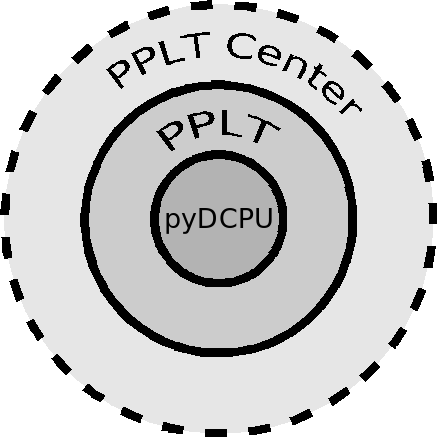
\includegraphics[scale=.5]{Reference/PPLTConcept01.png}
  %  \end{center}    
    \end{abstract}

    \tableofcontents


    \chapter{PPLT Reference}
\section{\module{PPLT} ---
        \textbf{P}otsdamer \textbf{P}rozess \textbf{L}eit \textbf{T}echnik}

\declaremodule{}{PPLT}
\moduleauthor{Hannes Matuschek}{hmatuschek@gmx.net}
\modulesynopsis{The PPLT is a framework for master/slave based communication.}

The \module{PPLT} builds an abstraction layer over the core library 
(\module{pyDCPU}). With the PPLT you can easily handle abstract devices and 
server instead of handle with several core modules. Like the core-library the 
PPLT has only one class called \code{System}. After instancing this class, all
work can be done by calling the methods of this object.

\section{Class description}
\begin{classdesc}{System}{\optional{BasePath}, \optional{CoreLogLevel}, 
\optional{PPLTLogLevel}, \optional{LogFile}, \optional{Syslog}, 
\optional{Lang}, \optional{AltLang}}
This is the all-in-one class. If this class will be instanced the complete 
PPLT system will be loaded. Meaning searching plug-ins (modules), loading 
user-database, starting core-system, etc...

The argument \var{BasePath} specifies the path of all PPLT related stuff. This 
is by default \code{sys.exec\_prefix+'/PPLT'}. Under Windows this is the folder 
where you've installed Python under \UNIX this should be some thing like 
\code{/usr/local/PPLT}. If you miss this argument, the default path will be 
used.

The argument \var{CoreLogLevel} specifies the log-level for the core library. 
This should be one of \code{off}, \code{fatal}, \code{error}, \code{warning}, 
\code{info}, \code{debug}.  If you select \code{debug} a lot of (not always 
useful) messages will be logged and \code{off} switches the logging off. 
By default the logging level \code{info} will be used. If you miss this 
argument, the default value will be used.

The argument \var{PPLTLogLevel} specifies the log-level of the PPLT library. 
This should be one of \code{off}, \code{fatal}, \code{error}, \code{warning}, 
\code{info}, \code{debug}. If you select \code{debug} a lot of (not always 
useful) messages will be logged and \code{off} switches the logging off. 
By default the logging level \code{info} will be used. If you miss this 
argument, the default value will be used.

The argument \var{LogFile} specifies the file,  where the logging messages are
written to. If you missed this argument, there were no messages written to any
file, all messages were send to screen (\code{stderr}). 

The boolean argument \var{SysLog} specifies if the messages should be send to
the local \code{syslog}-daemon. 
\begin{notice}
This argument overwrites the optional argument \var{LogFile}. If \var{SysLog}
it \code{True} no messages were written into any file nor send to screen!
\end{notice}
By default this argument if \code{False}. If you missed this argument, the 
default will be used.

The argument \var{Lang} specifies the primary language the system will use for
module description. This option do not change the language of the logging 
messages (they are not translated). This option is not important for normal
usage of the PPLT. By default \code{'en'} will be used.

The argument \var{AltLang} specifies the alternative language to be used
for module description. This should be always \code{'en'}. \textbf{Do not 
change until you know what you do.} 

If the primary language can not be found, the alternative will be used. 
\end{classdesc}




\section{Methods of \class{System}}
In this section I will describe the methods of the \class{System}-class. I 
will not list all available methods, because there are more then 60 of it. Some
of them are only useful if you want to write a GUI application like the
\emph{PPLT Center}. But you can get a short help over all methods by calling
\code{pydoc PPLT.System}. 


\subsection{Device methods}
\begin{methoddesc}[System]{LoadDevice}{DeviceName, Alias, Parameters}
This is one of the most important methods. With this method you can load and
setup a device. This method loads the device \var{DeviceName} as \var{Alias}. 
The alias will be used later to specify this device, for example if you want
to connect a symbol to this device or unload the device.

The argument \var{DeviceName} specifies the full qualified device name. All
devices (and servers) are grouped by classes. A full qualified device name
consists always of all classes and the name divided by a single dot. For
example \code{'PLC.Panasonic-FPX'}.

The argument \var{Alias} specifies the alias the device will get after being
loaded. By this alias you will identify the device later.

The attribute \var{Parameters} specifies the parameters the device needs to be
set up successfully. This should be a dict with key-value pairs. The key 
is the parameter name and the value should be the parameter-value. For example:
\code{\{'Port':'0', 'Address':'123'\}}.
\begin{notice}
All parameter names and also \textbf{all} parameter values are strings!
\end{notice}

This method will return \code{Ture} on success an \code{False} on error.
\end{methoddesc}


\begin{methoddesc}[System]{UnLoadDevice}{Alias}
This method unload and destroy the given device. 

The argument \var{Alias} specifies the alias of the device you want to be
unloaded. This is the alias you've set at the \method{LoadDevice} 
method-call.

This method returns \code{True} on success and \code{False} on error.
\end{methoddesc}


\begin{methoddesc}[System]{GetFQDeviceName}{Alias}
This method returns the full qualified device name of the device loaded as
\var{Alias}.

The attribute \var{Alias} specifies the alias of the loaded device. This is
the alias you've set at the \method{LoadDevice} method-call.

This method returns a string containing the full qualified device name or non 
if the alias if not a device or not loaded.
\end{methoddesc}


\begin{methoddesc}[System]{GetDeviceParameters}{Alias}
This method will return the parameters the device was loaded with. This method
will return a dict on success or \code{None} on error.
\end{methoddesc}


\subsection{Server methods}
This section describes all methods to handle servers, like starting, stopping, ... 

\begin{methoddesc}[System]{LoadServer}{ServerName, Alias, DefaultUser, Parameters\optional{, Root}}
This method loads and setup a server. 

The argument \var{ServerName} specifies the full qualified server name. Full 
qualified means that all classes and the name are given, divided by a single 
dot (like: \code{Web.PPLTWebServer}).

The argument \var{Alias} specifies the alias the server will have after 
being loaded. By this alias you will identify the server later, for example 
to unload this server.

The argument \var{DefaultUser} specifies the the user, the server will run as. 
By this option you can assign rights to a server, that doesn't know any 
authentication. By default, a server should support a authentication but 
sometimes the used protocol doesn't (for example JVisu). For this kind of 
server this option is useful.

The argument \var{Parameters} specifies the parameters the server will be 
loaded with. This should be a dict with the parameter name as key (string)
and the parameter value as value (also a string!). If a server doesn't needs
any parameters, please set \var{Parameters} to \code{None} or to and empty 
dict (\code{\{\}}). 

The optional argument \var{Root} specifies the server-root of this server. 
By default (\var{Root}=\code{'/'}) the whole symbol-tree will be accessible
by this server. But if you want to export only a specific folder of the 
symbol-tree you can specify this folder with the \var{Root} argument. So
if \var{Root}=\code{'/test'} only the content of the folder \code{'/test'}
will be accessible by this server.

This method returns \code{True} on success and \code{False} else.
\end{methoddesc}


\begin{methoddesc}[System]{UnLoadServer}{Alias}
This method will stop and destroy a server loaded with \method{LoadServer}.

The attribute \var{Alias} specifies the server you want to stop. This is the 
alias you've defined on loading the server with \method{LoadServer}.

This method will return \code{True} on success and \code{False} else.
\end{methoddesc}


\begin{methoddesc}[System]{GetFQServerName}{Alias}
This method will return the full qualified server-name of the loaded server
by his alias. 

The argument \var{Alias} specifies the alias of the server. This is the alias
you have defined on loading by the \method{LoadServer} method.

This method returns a string on success or \code{None} on error.
\end{methoddesc}


\begin{methoddesc}[System]{GetServerParameters}{Alias}
This method will return the dict of parameters the server was loaded with. 
This is the parameter dict, you have defined on loading the server with 
\method{LoadServer}.

The argument \var{Alias} specifies the alias of the loaded server. This is
the alias you have defined on loading the server with \method{LoadServer}.

This method will return a dict or \code{None} on error. This method will
return an empty dict even if you've loaded the server with no parameters.
\end{methoddesc}


\begin{methoddesc}[System]{GetServerRoot}{Alias}
This method will return the server root of a loaded server. This is the 
server root you have defined on loading the server with \method{LoadServer}.

The server root is the base folder in the symbol-tree the server can access. 
Only folders and symbols laying under this folder are accessible by this 
server.

The argument \var{Alias} specifies the alias of the loaded server. This is the
alias you have defined on loading the server with \method{LoadServer}. 

This method will return a string on success or \code{None} on error.
\end{methoddesc}


\begin{methoddesc}[System]{GetServerDefaultUser}{Alias}
This method will return the default-user the server is running with. This is
the username you have defined on loading the server with \method{LoadServer}.

If specified, the server will run with the rights of the default user. This is
necessary, because there are some servers which don't know any authentication!

The argument \var{Alias} specifies the alias of the loaded server. This is the 
alias you have defined for this server on loading with \method{LoadServer} 
call.

This method will return a string on success or \code{None} on error.
\end{methoddesc}


\subsection{Symboltree methods}
In the following section I will describe all methods for handling the symbol-tree. 
Like creating folder and symbols, moving them, ...

All methods, that working with the access-rights of a symbol or folder
are using following scheme to encode the rights:

\begin{center}
\begin{tabular}{|c|cc||c|cc||c|cc|} \hline\hline
\bf{Own} & $r$&$\not r$&\bf{Grp}&$r$ & $\not r$ & \bf{Any} & $r$ & $\not r$\\\hline
$w$ & 6 & 2 & - & 6 & 2 & - & 6 & 2 \\
$\not w$ & 4 & 0 & - & 4 & 0 & - & 4 & 0 \\\hline\hline
\end{tabular}
\end{center}
The access-right is represented as a string of 3 numbers each number specifies 
a access right. The first number specifies the right of the owner of the 
symbol or folder. The second specifies the right of the group assigned to the 
symbol/folder.  The last number specifies the right of everyone who not 
belongs to the assigned group nor being the owner. To en/decode the 
representation you can use the table above.


\begin{methoddesc}[System]{CreateFolder}{Path\optional{, Modus}\optional{, Owner}\optional{, Group}}
This method will crate a new folder (at \var{Path}) at the symbol-tree. 
Optional you can set the rights of this folder by the arguments \var{Modus}, 
\var{Owner}, \var{Group}. If the folder was successfully created, the method 
returns \code{True} else it returns \code{False}.

The argument \var{Path} specifies the \textbf{complete} path of the folder, 
you want to create. You cant create folders relative to an other because the 
system don't know the relative.

The argument \var{Modus} specifies the modus the folder will have. By this 
argument you can set the access rights of this folder. The argument should be
a string with an octal integer in it. Meaning something like this: \code{'600'}.
Each number of the integer represents the encoded right. For the owner of the
folder (1st number), the group assigned to the folder (2nd number), and any other
(last number). For encoding you can use table above. 
By default the modus will be \code{'600'}. This denotes that only the owner 
of the folder have read/write access. (By default this will be the system admin.)

The argument \var{Owner} specifies the owner of the folder. This have to be 
existing user-name. 

The argument \var{Group} specifies the group, the folder will be assigned to. 
This have to be an existing group-name.

\begin{notice}
You can reset the modus, owner and group later by calling 
\method{ChangeModus}, \method{ChangeOwner} or \method{ChangeGroup}.
\end{notice}
\end{methoddesc}


\begin{methoddesc}[System]{DeleteFolder}{Path}
With this method you can delete an \textbf{empty} folder of the symbol-tree.

The argument \var{Path} specifies the \textbf{full} path to the folder you want to
delete. This is the path you've set on create the folder by 
\method{CreateFolder} method-call.

This method returns \code{True} on success an \code{False} else.
\end{methoddesc}


\begin{methoddesc}[System]{MoveFolder}{From, To}
This method moves a folder to an other or to the root of the symbol-tree.

The argument \var{From} specifies the \textbf{full} path of the folder you want
to move. The argument \var{To} specifies the \textbf{full} path of the destination 
folder you want the source folder to be moved to. Of cause, the destination folder
can't be a sub-folder of the source.

This method returns \code{True} on success an \code{False} on error.
\end{methoddesc}


\begin{methoddesc}[System]{ListFolders}{Path}
This method returns the names of all folders in \var{Path}.

The argument \var{Path} specifies the \textbf{full} path of the parent-folder
you want to list it's sub-folders. If you want to list the root path, please 
set \var{Path}=\code{'/'}.

The method returns a list of strings on success or \code{None} on error. 
This method will return an empty list if the given folder doesn't contain 
any sub-folders.
\end{methoddesc}


\begin{methoddesc}[System]{CreateSymbol}{Path, Slot, Type, \optional{, Modus}\optional{, Owner}\optional{, Group}}
This method creates a new symbol on path \var{Path} connected to the slot \var{Slot} and associated with the type
\var{Type}. Optional you can set the owner, group and access rights of the new symbol.

The argument \var{Path} specifies the full path to the symbol that should be 
created. \textbf{Note}: All folder on this path must exist! 

The argument \var{Slot} specifies the full qualified slot name of the slot you
want the symbol to be connected to. Thy typical format of a slot-name is 
\code{DEVICEALIAS::NAMESPACE::SLOT}. Please substitute the alias of the device
the symbol will be attached to with \code{DEVICEALIAS}. You can find the 
namespaces and slot/slot-ranges the device provide at the Chapter 
\emph{PPLT Modules}.

The argument \var{Type} specifies the type-name the symbol will associated 
with. This should be one of \code{'Bool'}, \code{'Integer'}, 
\code{'uInteger'}, \code{'Float'}, \code{'Double'}, \code{'String'}, 
\code{'ArrayOfBool'}, \code{'ArrayOfInteger'}, \code{'ArrayOfuInteger'},
\code{'ArrayOfFloat'}, \code{'ArrayOfDouble'}, \code{'ArrayOfString'} and
\code{'Raw'}.

The optional argument \var{Modus} specifies the access-right of the new symbol.
This should be a string (i.e. \code{'600'}) containing an octal integer 
representing the access-rights like described above.

The optional argument \var{Owner} specifies the owner of the symbol. This
should be a string containing a existing user-name. By default this will be
the user marked as super-user.

The optional argument \var{Group} specifies the group, the symbol will be 
attached to. This should be a string containing the name of an existing 
group. By default this will be the group of the super-user.

This method will return \code{True} on success or \code{False} else.
\end{methoddesc}


\begin{methoddesc}[System]{DeleteSymbol}{Path}
This method will remove a symbol from the symbol tree.

The argument \var{Path} specifies the \textbf{full} path
to the symbol you want to remove. 

This method will return \code{False} on error or \code{True} on success.
\end{methoddesc}


\begin{methoddesc}[System]{MoveSymbol}{From, To}
This method moves a symbol from path \var{From} into the folder specified by 
\var{To}.

The argument \var{Specifies} the symbol you want to move and the argument 
\var{To} specifies the destination folder. The destination folder have to exist.

This method return \code{False} on error or \code{True} on success.
\end{methoddesc}


\begin{methoddesc}[System]{ListSymbols}{Path}
This method will list all symbols of the folder specified by \var{Path}.

The argument \var{Path} specifies the folder.

This method will return a list of strings, even if the folder doesn't contain 
any symbols (in this case the method will return an empty list). The method
will return \code{None} on error.
\end{methoddesc}


\begin{methoddesc}[System]{GetValue}{Path}
This method returns the value of the symbol specified by the argument 
\var{Path}. 

This method will return any value or a list of values on success or 
\code{None} on error.
\end{methoddesc}


\begin{methoddesc}[System]{SetValue}{Path, Value}
This method will set the value of the symbol specified by \var{Path} to 
\var{Value}.

The argument \var{Path} specifies the symbol, you want to set. The argument 
\var{Value} specifies the value (or even the list of values) you want to set 
to the symbol.

This method will return \code{True} on success or \code{False} on error.
\end{methoddesc}


\begin{methoddesc}[System]{GetSymbolSlot}{Path}
This method returns the slot-name, a symbol is connected to. 

The argument \var{Path} specifies the \textbf{full} path
to the symbol.

This method returns a string or \code{None} on error.
\end{methoddesc}


\begin{methoddesc}[System]{GetSymbolType}{Path}
This method returns the type-name of a symbol. The argument \var{Path} 
specifies the \textbf{full} path to the symbol. This method returns 
\code{True} on success or \code{None} on error.
\end{methoddesc}


\begin{methoddesc}[System]{GetSymbolTimeStamp}{Path}
This method returns the timestamp of the value of a given symbol. The argument
\var{Path} specifies the full path to the symbol. \textbf{Note}: This method
will return the timestamp of the last update of the symbol-value. This is not 
always the timestamp of the last \emph{successful} update. This method will 
return a float (seconds since epoch) on success or \code{None} on error.
\end{methoddesc}


\begin{methoddesc}[System]{GetOwner}{Path}
This method will return the owner-name of a symbol. The argument
\var{Path} specifies the \textbf{full} path to the symbol. This method will
return a string on success or \code{None} on error.
\end{methoddesc}


\begin{methoddesc}[System]{ChangeOwner}{Path, Owner}
This method sets the owner of a symbol or folder. The argument \var{Path} 
specifies the \textbf{full} path to the symbol/folder. The argument 
\var{Owner} specifies the name of the new owner. This must be an existing 
username! This method will return \code{True} on success or \code{False} on
error.
\end{methoddesc}


\begin{methoddesc}[System]{GetGroup}{Path}
This method will return the name of the group a symbol or folder is attached 
to. The argument \var{Path} specifies the \textbf{full} path of the 
symbol/folder. This method will return a string containing the group-name
or \code{None} on error.
\end{methoddesc}


\begin{methoddesc}[System]{ChangeGroup}{Path, Group}
This method sets the group a symbol or folder is attached to. The argument
\var{Path} specifies the \textbf{full} path to the symbol/folder. The argument
\var{Group} specifies the group-name, the folder/path will be attached to. This
must be a existing group.
\end{methoddesc}


\begin{methoddesc}[System]{GetModus}{Path}
This method will return the access-rights of the given symbol or folder.
The argument \var{Path} specifies the \textbf{full} path to the symbol/folder.
This method will returns a string formated as described above or \code{None}
on error. 

To process this string by your script, I recommend you to convert this string 
into a integer and then working with bit operations on it like the following 
example thats extract the rights of owner, group and other into a tuple of 
integers.
\begin{verbatim}
import PPLT
import string

pplt = PPLT.System()
[...]
tmp = pplt.GetModus("/Path/To/Symbol");
if tmp:
    tmp = string.atoi(tmp,8)    # convert string to int on base 8.
    other = tmp & 0x7;
    group = (tmp>>3) & 0x7;
    owner = (tmp>>6) & 0x7;
\end{verbatim}    
\end{methoddesc}


\begin{methoddesc}[System]{ChangeModus}{Path, Modus}
This method will set the access rights of owner, group and other
of a given symbol or folder. The argument \var{Path} specifies the 
\textbf{full} path to the symbol/folder. The argument \var{Modus} specifies
the access-rights. This should a string containing the 3 octal numbers 
specifying the rights like described above. This method will return 
\code{True} on success or \code{False} on error.
\end{methoddesc}


\begin{methoddesc}[System]{ClearSymbolTree}{\optional{Path}}
This method will clear (remove all) elements from the whole symbol-tree or
optional down from the given \var{Path}. This method will return 
\code{True} on success or \code{False} on error.
\end{methoddesc}




\subsection{Misc. methods}
\begin{methoddesc}[System]{LoadSession}{FileName}
This method will load a complete session from the given file. Note, this file
have to be in the PSF format described in the chapter 
\emph{PSF --- PPLT Session File}. The argument \var{FileName} specifies the
filename of the session file to load.
\begin{notice} 
The current session will be lost! 
\end{notice}
This method will return \code{True} on success and \code{False} on error.
\end{methoddesc}


\begin{methoddesc}[System]{SaveSession}{FileName}
This method will save the current session to the given file. The used
format is the PSF format described in the chapter 
\emph{PSF --- PPLT Session File}. The argument \var{FileName} specifies
the file to save the session to. The method will return \code{True} on 
success an \code{False} on error.
\end{methoddesc}


\begin{methoddesc}[System]{StopAll}{}
This method stops the whole PPLT system and reset it to the init state by calling  the 
methods \method{ClearSymbolTree}, \method{StopDevices} and
\method{StopServers}. This method will return \code{True} on success or
\code{False} on error.
\end{methoddesc}


\begin{methoddesc}[System]{StopDevices}{}
This method will stop and unload all loaded devices. The method can be used to
shutdown the PPLT system. The method will return \code{True} on success or 
\code{False} on error.
\end{methoddesc}


\begin{methoddesc}[System]{StopServers}{}
This method will stop all loaded servers and unload them. This method can be used 
to shutdown the PPLT system. This method will return \code{False} on error or 
\code{True} on success.
\end{methoddesc}


    \newcommand{\PPLTModDesc}[1]{\subsection{#1}\indexii{PPLT Module}{#1}}
\newcommand{\PPLTMod}[1]{\code{#1}}
\newcommand{\PPLTDev}[1]{\PPLTMod{#1}}
\newcommand{\PPLTSrv}[1]{\PPLTMod{#1}}


\chapter{PPLT Module Reference}
In this chapter i will describe all avaiable PPLT modules. A PPLT module is server or device, that consists of one or more
so called \textit{core modules}. The main idea of having an abstract device instead of many (more flexible) core modules, is the
easy handleing of a (single) simple device insted of dealing with a couple of modules. 

Technical, a PPLT module is an XML file describing how to combine the coremodules to get the support for
a special device or system. 

For example; If you want to access the markers of a Siemens SIMATIC S7-200 
by the PPI bus you have to load the coremodule for the serial interface, the module for the PPI bus and
at the end the module for the S7-200. Each of these module has a couple of parameters, to get the 
system running. Sometimes you'll need to know a lot about the bus-system to know how to setup the 
single core modules. Instead of this you can load a single PPLT module called \PPLTMod{'PLC.S7-200'}. This 
module needs only 3 paremeters to setup the support for the S7. This would be much easier.




\section{Devices}
This section describe all devices. All devices are grouped in classes. The name of the device consists of
the full class path and the name of the specific device, devided by a singel dot. For example: 
\PPLTMod{Debug.RandomGenerator}.






\PPLTModDesc{Debug.RandomGenerator}
The PPLT module \PPLTMod{Debug.RandomGenrator} implements a simple random gererator, thats provide random
value in different types. This is the simplest device. It needs no additional python libraries nor any 
special hardware to run. So it can easiely be used to test the PPLT.

\subsubsection{Parameters}
This device needs no parameters to be setted up. 

\subsubsection{Namespaces and slots}
This device provide only one namespace called \code{Generatior}. This namespace conatains
4 slots. Each slot provide a random value for a different type. And different range.

\paragraph{Slots of namespace \texttt{Generator}:}
Each slot retuns a value of the type by his name.
\begin{tableiii}{l|l|l}{textrm}{Slotname}{Type}{Description}
\lineiii{Bool}
        {Bool}
        {Returns randomly \code{True} or \code{False}}
\lineiii{uInteger}
        {uInteger}
        {Returns a unsigned integer between 0-100.}
\lineiii{Float}
        {Float}
        {Returns a floatingpoint number between 0-1.}
\lineiii{Double}        
        {Double}
        {Returns a floatingpoint number betwenn 0-1.}
\end{tableiii}

\subsubsection{Example}
\begin{verbatim}
import PPLT

pplt = PPLT.System();
pplt.LoadDevice("Debug.RandomGenerator", "alias", {})
\end{verbatim}

This example loads the device as \code{"alias"}. This alias should be replaced by the alias you want to give to
the loaded device-instance. You'll need this alias later to unload the device or to connect symbols to it.









\PPLTModDesc{Mobile.GSMMobilePhone}
This device can access a GSM compatible mobile phone by the serial interface. It can read out
some status infromation  like batterielevel, signal quality, etc... In the near future this 
device will also learn to send SMS. 

\begin{notice}
Because this device uses the serial interface, you'll need to have the \module{pyserial} 
python library installed. Please check this before you use this device.
\end{notice}

\subsubsection{Parameters}
This device needs some parameters\footnote{Please note, that all 
parameter-value have to be strings.} be setted up. At least you have to set 
the port (number of the serial interface) where the mobile phone is connected 
to the computer. Additional you can set the speed (in baud) of the interface.
\begin{tableiii}{l|l|l}{textrm}{Parameter}{Description}{Default value}
\lineiii{Port}
        {Sets the number of the serial interface. Note: COM1 (ttyS0) = 0, COM2 = 1, ...} 
        {"0"}
\lineiii{Speed}
        {Sets the speed in baud of the serial interface.}
        {"9600"}
\end{tableiii}

\subsubsection{Namespaces and slots}
This device provides only one namespace called \code{GSM}. This namespace 
contains 6 slots. These slots provides status information about the 
mobilephone.

\paragraph{Slots of namespace \texttt{GSM}:}
There are several slots, each providing a status value of the mobile phone.
\begin{tableiii}{l|l|l}{textrm}{Slotname}{Type}{Description}
\lineiii{battery}
        {uInteger}
        {The battery level in percent.}
\lineiii{network}
        {uInteger}
        {The networkstatus of the mobile phone.}
\lineiii{quality}
        {uInteger}
        {The signal quality.}
\lineiii{errorrate}
        {uInteger}
        {The errorate of the networkconnection.}
\lineiii{manufacturer}
        {String}
        {Manufacturer name.}
\lineiii{model}
        {String}
        {Modelname.}
\end{tableiii}


\subsubsection{Example}
This example loads the \PPLTDev{GSMMobilePhone} module on port 0 (COM1) with speed 9600 baud as the alias \code{'gsm'}. Then it creates a symbol \code{/manu}
that will be connected with the \code{manufacturer} slot of the device. And at the end the symbol will be readed out.
\begin{verbatim}
import PPLT

pplt = PPLT.System()
pplt.LoadDevice("Mobile.GSMMobilePhone","gsm",{'Port':'0', 'Speed':'9600'})
pplt.CreateSymbol("/manu","gsm::GSM::manufacturer","String")

print pplt.GetValue("/manu")
\end{verbatim}






\PPLTModDesc{PLC.Panasonic-FPX}
This device implements the support for the Panasonic FP0 and FP2 PLCs. With 
this device you can read/write the markers of the PLC connected to the PC by 
the so called ToolPort or over the Mewtocol-BUS. 

You can also acces a FP0 by the FP-WEB server, who tunnels the toolport to a 
TCP port by the \PPLTDev{PLC.Panasonic-FPWEB} device. 

\subsubsection{Parameters}
This device needs at least the number of the serial interface and
the Mewtocol-address of the PLC.
\begin{notice}
All parameter-values have to be strings!
\end{notice}

\begin{tableiii}{l|p{10cm}|l}{textrm}{Parameter}{Description}{Default value}
\lineiii{Port}
        {The number of the serial interface, where the PLC is connected to. (Note: COM1(ttyS0) = 0, COM2(ttyS1) = 1,...)}
        {}
\lineiii{Address}
        {The Mewtocol-address of the PLC in the Mewtocol BUS. Note: If you use
        the ToolPort to access the PLC you can take any number between 0 and
        255. (The mashine will ignore the address.)}
        {}
\end{tableiii}

\subsubsection{Namespaces and slots}
Also this device provide only one namespace called \code{Marker}. This 
namespace contains the slot \var{STATUS} and the slotrange \var{Marker}. A 
slotrange is a placeholder of a couple of slots. In this conectext it is a
placeholder for all markers of the PLC. So if you want to access a marker,
for example \code{Y0}\footnote{The first output pin.}, you should replace
the slotrange by the name of the marker: \code{Alias::Marker::Y0}. 
You have to figure out the type of the slot by your self, if you use
a slotrange! But so far, if you access a boolean marker, use \code{'Bool'}
if you access an integer marker (byte, word, double word) please use 
the unsigned integer \code{'uInteger'} as type.
\begin{notice}
Please use uppercase for the name of the marker!
\end{notice}

\paragraph{Slots of the namespace \texttt{Marker}:}
There is only on slot in this namespace. But you can access all markers 
of the PLC like described above.
\begin{tableiii}{l|l|p{10cm}}{textrm}{Slotname}{Type}{Description}
\lineiii{STATUS}
        {Bool}
        {This slot controlls the status of the PLC, if this slot is 
        \code{True} the PLC is in the \emph{Run} mode if it is
        \code{False} it is in the \emph{Stop} mode. You can also
        set the mode by writing into this slot.}
\end{tableiii}

\subsubsection{Example}
In this example I show you how to setup the \PPLTDev{PLC.Panasonic-FPX} 
device. Then I create a symbol for the status bit and one for the first 
output-bit (Y0). Then I set the PLC into the \emph{Run} mode. At the end the
script willwait for a second and then it will set the first output-bit
to \code{True}.

\begin{verbatim}
import PPLT
import time

pplt = PPLT.System()
pplt.LoadDevice("PLC.Panasonic-FPX","fp0",{"Port":"0", "Address":"1"});

pplt.CreateSymbol("/stat","fp0::Marker::STATUS","Bool");
pplt.CreateSymbol("/y0", "fp0::Marker::Y0", "Bool");

# set the PLC into run-mode:
pplt.SetValue("/stat",True);

# wait a second:
time.sleep(1);

# set Y0 to 1:
pplt.SetValue("/y0",True);
\end{verbatim}






\PPLTModDesc{PLC.FPWEB}
This device implements the access to a Panasonic FP0 or FP2 over the toolport 
tunneled by the Panasonic FP-WEB server. This device is quiet equal to the
\PPLTDev{PLC.Panasonic-FPX} device. So it provides the same namespace with
the same slots and slotranges.

If you want to access the FP0 or FP2 directly by the toolport, please use
the \PPLTDev{PLC.Panasonic-FPX} device instead.

\subsubsection{Parameters}
This device needs only two parameters to be setted up correctly. The nework
address of the webserver and the Mewtocol address of the PLC.
\begin{tableiii}{l|p{10cm}|l}{textrm}{Parameter}{Description}{Default value}
\lineiii{NetAddr}
        {The network address of the webserver and the port of the tunneled
        toolport in the format \code{ADDRESS:PORT}. For example 
        \code{10.1.1.4:9094}.}
        {}
\lineiii{MewAddr}
        {The Mewtocol address of the PLC connected to the webserver. In
        the normal case, the webserver will be pluged on the toolport
        of the PLC so this number could be any between 0 and 255 because
        the PLC will ignore the destination address field.}
        {\code{1}}
\end{tableiii}

\subsubsection{Namespaces and slots}
Also this device provide only one namespace called \code{Marker}. This 
namespace contains the slot \var{STATUS} and the slotrange \var{Marker}. A 
slotrange is a placeholder of a couple of slots. In this conectext it is a
placeholder for all markers of the PLC. So if you want to access a marker,
for example \code{Y0}\footnote{The first output pin.}, you should replace
the slotrange by the name of the marker: \code{Alias::Marker::Y0}. 
You have to figure out the type of the slot by your self, if you use
a slotrange! But so far, if you access a boolean marker, use \code{'Bool'}
if you access an integer marker (byte, word, double word) please use 
the unsigned integer \code{'uInteger'} as type.
\begin{notice}
Please use uppercase for the name of the marker!
\end{notice}

\paragraph{Slots of the namespace \texttt{Marker}:}
There is only on slot in this namespace. But you can access all markers 
of the PLC like described above.
\begin{tableiii}{l|l|p{10cm}}{textrm}{Slotname}{Type}{Description}
\lineiii{STATUS}
        {Bool}
        {This slot controlls the status of the PLC, if this slot is 
        \code{True} the PLC is in the \emph{Run} mode if it is
        \code{False} it is in the \emph{Stop} mode. You can also
        set the mode by writing into this slot.}
\end{tableiii}

\subsubsection{Example}
In this example I will show you how to load the \PPLTDev{PLC.FPWEB} device. 
The script will then do the same like the example script of the 
\PPLTDev{PLC.Panasonic-FPX} device. It will create 2 symbols, one for
the status bit and one for the first output bit (Y0), then it will
set the PLC into the \emph{Run} mode and will set the Y0 to True.

\begin{verbatim}
import PPLT
import time

pplt = PPLT.System()
pplt.LoadDevice("PLC.FPWEB","fp",{"NetAddr":"10.1.1.100:9094", "MewAddr":"1"});

pplt.CreateSymbol("/stat","fp::Marker::STATUS","Bool");
pplt.CreateSymbol("/y0", "fp::Marker::Y0", "Bool");

# set the PLC into run-mode:
pplt.SetValue("/stat",True);

# wait a second:
time.sleep(1);

# set Y0 to 1:
pplt.SetValue("/y0",True);
\end{verbatim}






\PPLTModDesc{PLC.S7-200}
This device implements the access to a Siemens SIMATIC 
S7-200\footnote{I've only tested it with a S7-200 maybe other also working 
fine. Please let me know if it woks for you.} PLC. With this device you can 
read/write the markers of a Siemens PLC. Additional you can get some 
statistical values about the PPI BUS line muber of bytes send/recived.
\begin{notice}
This device implements only the access over a PPI cable!
\end{notice}


\subsubsection{Parameters}
To setup the device you need to set at least the number of the serial 
interface used and the PPI address of the PC and the PLC.
\begin{tableiii}{l|l|l}{textrm}{Parameter}{Description}{Default value}
\lineiii{Port}
        {Number of the serial interface to be used. (COM1=0, COM2=1,...)}
        {0}
\lineiii{PCAddr}
        {The PPI address of the PC. This would normaly 0(Master).}
        {0}
\lineiii{S7Addr}
        {The PPI address of the PLC. Normaly a number between 0 and 32.}
        {2}
\end{tableiii}

\subsubsection{Namespaces and slots}
This device provides two namespaces. One called \code{PPIStatistic}, provides 
slots for statistical values about the PPI BUS. The other one called 
\code{Marker} provides a slotrange named \code{Merkers}.

A slotrange is a placeholder for a whole range of slots. In this case it
is a placeholder for all markers of the PLC. So if you want to access a
marker, please replace the slotrange by the name of the marker you want 
to use. For example if you want to connect a symbol to the marker
\code{SMB28} please use \code{"ALIAS::Marker::SMB28"} as the 
slotname\footnote{Please use only uppercase letters for the merkername.}. 

\paragraph{Slots of the namespace \texttt{PPIStatistic}:}
This namespace contains some slot for statistical information about the 
underlaying PPI BUS. 
\begin{tableiii}{l|l|p{10cm}}{textrm}{Slotname}{Type}{Description}
\lineiii{read\_data}
        {uInteger}
        {This slot returns the nuber of recived bytes.}
\lineiii{write\_data}
        {uInteger}
        {This slot returns the number of send bytes.}
\lineiii{read\_speed}
        {uInteger}
        {Returns the number of bytes recived per second.}
\lineiii{write\_speed}
        {uInteger}
        {Returns the number of bytes send per second.}
\lineiii{error}
        {uInteger}
        {Counts the transpor.......}
        
\subsubsection{Example}







\PPLTModDesc{Measure.AGILENT-5462X}
This device implements the access to a Agilent oscilloscope of the 5462X 
series. With this device you can contol the oscilloscope, for example you can
measure the frequency of a signal. This device supports only the serial
interface to the Agilent, GIPB or something like this is not supported.

\subsubsection{Parameters}
\subsubsection{Namespaces and slots}
\subsubsection{Example}













\section{Servers}
In this section i'll describe all available servers for the PPLT system.
(some more text...)





\PPLTModDesc{Web.PPLTWebServer}
\subsubsection{Parameters}
\subsubsection{Example}






\PPLTModDesc{Visu.JVisuServer}
\subsubsection{Parameters}
\subsubsection{Example}



\PPLTModDesc{RPC.SimpleExport}
\subsubsection{Parameters}
\subsubsection{Example}




    
    \chapter{Core reference}
\section{\module{pyDCPU} --- 
        \textbf{Py}thon \textbf{D}ata \textbf{C}ollect and \textbf{P}rocess \textbf{U}nit}

\declaremodule{}{pyDCPU}       

\moduleauthor{Hannes Matuschek}{hmatuschek@gmx.net}


\modulesynopsis{This is the reference for the core-library of PPLT System.}

The \module{pyDCPU} module provides all needed core methods and functions, to
get a PPLT system running. The library implements the basic features like 
loading modules (Master/Exporter), manageing the symboltree 
(create/move/delete/chmod/chown/chgrp/...) and manageing the user
data base. Basicly the \module{pyDCPU} library provides all the functionality
of the PPLT system. 

\subsection{Concept} 
The core of the PPLT system have to provide all the functionality to access devices
by master-slave based communication channels and handle the values read back into
a central place. Also these values should be served to other applications, indipendent
from the interface the application use. So the core is splitted into three major parts.

\begin{figure}[ht]
    \centering
    \label{cDCPU}
    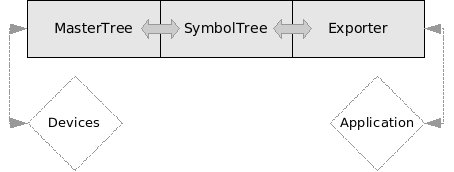
\includegraphics[scale=1]{cDCPU.png}
    \caption{Parts of the core.}
\end{figure}

The first called \textit{MasterTree}. This provide the access to the devices. The 
second part called \textit{SymbolTree} holds all values in a filesystem like 
hierachie. The last part, the \textit{Exporters}, serves the symboltree to other
applications like a visualisation. This concept is very common for this kind of 
problems. 

\subsubsection{The MasterTree}
To access the devices a master-slave based communication is often used. This are 
for example the common BUSes and also TCP/IP like networks. All these protocols
have one basic concept; they are seperable into layers. Each layer encapsulate 
an element of the communication.  For TCP/IP this is the famouse OSI reference 
model. So it is usefull to implement each layer of the communication channel
into separate modules to have the facility to reuse some of the modules. By
this you only need to implement these layers of the communication, that aren't
implemented yet to access a new device. For example if you want to access
a unsupported device that uses an allready implemented BUS you'll need only
to write a module that implements the command messages for this device.

A common way to seperate the communication is to differ between the used
interface, transport-protocol, and command-messages. The interface provides
the access to the BUS wardware, for example the serial-interface. The 
transport-protocol or BUS protocol uses the interface and generate valid 
messages that reaches the device. The module that generates the 
command-messages uses the transport-protocol to send the messages to the
device and to wait for an answer.  

\begin{figure}[ht]
    \centering
    \label{fig:cMasterTree}
    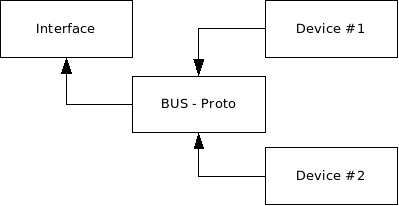
\includegraphics[scale=1]{cMasterTree.png}
    \caption{Scheme of MasterTree concept with shared interface and BUS modules.}
\end{figure}

An common cenario would be: You want to get a value from a device. So
you read from the module-object that implements the command messages.
This module will send a command-message over the BUS (protocol and interface)
to the device. Then the module will waits for an answer of the device
by reading from the BUS (over protocol and interface module). The
answer will be dispatched and you'll get the value.

If one module read from or writes to an other module the modules
will be locked and no other module can access these modules. By this way 
BUS collisions are avoided. And on the other hand if you want to access
two devices that are connected to the same BUS, you'll setup a 
MasterTree where the device-modules \#1 and \#2 share the modules for the 
interface and BUS. Now you see why the MasterTree is called a tree (forest 
would be better). The root of each tree is the interface and the leafes are 
the devices.

To get the all module work together a clear API between the modules have
to be defined, so that you don't have to adjust the modules to work together
with other/new modules. 

\subsubsection{The SymbolTree}
Once the access to the devices is seted up, you need to care about what values 
should be served. Each device will be able to provide a lot of different values
and a user or application don't know how to get a specific value. So you'll 
need a abstraction of the set of values. On the other hand, if you want to 
serve a lot of values you want to group the values by there sense and not by the
devices they are come from. So the idea of a \textit{filesystem} raises that holds 
the values in \textit{symbols} grouped in \textit{folders}, independent of the 
device the value was read from. At this point it will be usefull to control
who have access to a specific value (symbol). 

A symbol is usualy directly connected to a device-module. That means, if you 
want to get the value of the symbol, the symbol asks the device-module to read
the value from the device. But it is also possible to connect a symbol to a
module that implements a BUS protocol. By this you'll be able to tunnel the 
BUS to an other application of the internet. If you read out of such a symbol
you'll read directly from BUS and if you write into the symbol you'll write 
into the BUS. But be carefull with exporting the BUS to other networks, you
can't control what messages are sent over the BUS!

\subsubsection{Exporter}
The last part of the core exports the symboltree, or maybe a part of it, to
other applications. So the PPLT system is able to support a wide range of 
applications, independent of the protocol or interface the application
will use. Also the exporter are implemented as modules. But in this case
the comunication with the exporters are not seperated into seperate modules.
Each exporter is run into its own thread. So it is possible to handle
different applications with several instances at the same time. 


\section{Class description}
\begin{classdesc}{Core}{\optional{ModulePath, \optional{UserDBFile, \optional{LogLevel, \optional{LogFile, \optional{SysLog}}}}}}
This is the all-in-one class of the \module{pyDCPU}. All work like loding 
modules will be done by calling methods of this class. 

Creates a new core-instance. The optional argument \var{ModulePath} specifies
the basepath to the core-modules. If missed, the default path 
\texttt{sys.exec\_path+"/PPLT"} will be used. 

The argument \var{UserDBFile} specifies the filename of the used database to 
be loeded. If missed the default file 
(\texttt{sys.exec\_path+"/PPLT/UserDB.xml"}) will be used.


The argument \var{LogLevel} specifiy the loglevel and so the verbosity of the 
core. This shloud be one of (\code{'off'}, \code{'fatal'}, \code{'error'}, 
\code{'info'} or \code{'debug'}). Note that \code{'off'} switches the logging
off and \code{'debug'} will produce a lot of messages. 

In normal case all logging massages were printed on the screen (send to 
stderr) but with the arguments \var{LogFile} and \var{SysLog} you can 
manipulates this behavor. If the argument \var{LogFile} is given, this file 
will be used to log all messages to. Note, that if \var{LogFile} specified no 
messages are shown on stderr. If \var{SysLog} is \code{True} all log messages 
will be send to the local syslog-daemon. Note this argument overrides the 
setting of \var{LogFile} and also no messages were send to stderr.
\end{classdesc}

\section{Methods of \class{Core}}
\label{core-objects}
In the following section I will describe all methods of the \class{Core} 
class. 


\subsection{Mastertree methods}
\begin{methoddesc}[Core]{MasterTreeAdd}{ParentID, ModName, Address, Parameter}
This method loads an instance of a coremodule and adds it to the mastertree. 
The method returns the ID of the loaded mdoule. This ID is unique but if you 
load the same module with the same parameters, address and at the same parent, 
the ID of the allready loaded module will be returned. If an error accoures, 
the method will return \code{None}.

The argument \var{ParentID} specifies the parent-module (ID), the new loaded 
module will be attached to. If you set \var{ParentID} to \code{None} the 
module will be loaded as a root\footnote{A root-module has no parent module.}. 

The argument \var{ModName} specifies the full qualified name of the module. 
All modules are orgenized in classes and subclasses. A full qualified name 
would be a modulname with all classes and subclasses divided by single dots. 
For example: \code{Master.Interface.UniSerial} or \code{Master.Device.S7-200}.

The argument \var{Address} specifies the address used to connect the parent 
module. If there is no parent, meaning \var{ParentID} is \code{None}, or there
is no need to addressing the parentmodule, the argument \var{Address} should 
be \code{None}.

The argument \var{Parameter} specifies the parameter used to load (and setup) 
the module. This argument shlould be a dict.  The keywords are the parameters 
names (all strings) and the vlaues are the values of the singe parameter. \\ 
\note{All parameter values are strings!} If the module needs no parameters, 
please set \var{Parameter} to \code{None} or to an empty dict \code{\{\}}.
\end{methoddesc}


\begin{methoddesc}[Core]{MasterTreeDel}{ObjectID}
This method removes an (module-)object from the mastertree and destroy it. 
\note{The object mast have no chlidren, meaning no other objects  
are connected to this object.}

The argument \var{ObjectID} specifies the object you want to remove. This 
object ID is the ID you got by the \function{MasterTreeAdd()} method-call.

The method will return \code{True} if the object could be removed and destroyed 
and \code{False} otherwise.
\end{methoddesc}


\begin{methoddesc}[Core]{MasterTreeList}{ParentID}
This mehtod will list the IDs of all childen of the given moduleinstance. The argument \var{ParentID} specifies the 
ID of the moduleinstance, that children will be listed. 
\end{methoddesc}


\subsection{Symboltree methods}
\begin{methoddesc}[Core]{SymbolTreeCheckPath}{Path}
This method checks if the given \var{Path} exists. This method retuns  \code{True} if the given path is a folder or symbol
and \code{False} otherwise.
\end{methoddesc}


\begin{methoddesc}[Core]{SymbolTreeCreateFolder}{Path}
This method creates a folder. 

The argument \var{Path} specifies the full path to the folder, that will be creted. \note{The path should have the 
standrd Linux format like: \code{'/path/to/new\_folder'}.}

This method will return \code{Ture} if the folder was sucsessfully created and 
\code{False} otherwise.
\end{methoddesc}


\begin{methoddesc}[Core]{SymbolTreeCreateSymbol}{Path, ObjectID, \optional{Address}, \optional{Timeout}}
This method will creat a new symbol in the symboltree and connect it to the 
given Object.

The argument \var{Path} specifies the full path to the new symbol. This path 
should be in the standard Linux format like \code{'/path/to/new\_symbol'}.

The argument \var{ObjectID} specifies the object, the symbol will be connected
to. This is the ID you've got bach from a \function{MasterTreeAdd} call. You can 
connect a symbol to any object, but you'll not get allways usefull values back 
from this object. You can also connect the symbol to an object, that doesn't provide
any values, for example to a object of the \code{UniSerial} module to tunnel the
serial interface to an external application by the symboltree.

The optional argument \var{Address} specifies the address to be used to connect
to the object. To find out what addresses are provided by a specific module,
please look at the \textit{Core Modules Reference}. Of the address is obmitted,
no address will be used to connect to the object. In the most cases this means
to connect to the data chanel of the module. 

The optional argument \var{Timeout} specifies the cacheing time for the symbol in
seconds. The deault value is 0.5s.
For this time the last read value is returned instead of reread the value each 
time. By this it is possible to reduce the trafic on BUS if may clients access 
the symbols.
\end{methoddesc}


\begin{methoddesc}[Core]{SymbolTreeDeleteFolder}{Path}
This method will remove the given folder. This folder should be empty before removing it.

The argument \var{Path} specifies the path of the folder that will be removed. 

This method returns \code{True} on success and \code{False} on error.
\end{methoddesc}


\begin{methoddesc}[Core]{SymbolTreeDeleteSymbol}{Path}
This method will remove a symbol from the symboltree. 

The argument \var{Path} specifies the full path to the symbol, that will be removed.
This path should be in the standard Linux format like: \code{'/path/to/symbol'}.

This method will return \code{True} on success and \code{False} otherwise.
\end{methoddesc}


\begin{methoddesc}[Core]{SymbolTreeListFolder}{Path}
This method list all folders in the folder pointed by \var{Path}.

The argument \var{Path} specifies the full path to the folder, that subfolders
will be listed. 
\note{If you want to list all folders at the 
root-folder, you shloud use \code{'/'} as path.}

The method returns a list of strings or \code{None} if the path doesn't exists. The method will
return an empty list if the folder has no subfolders.
\end{methoddesc}


\begin{methoddesc}[Core]{SymbolTreeListSymbols}{Path}
This method will list all symbols in the folder pointed by \var{Path}.

The argument \var{Path} specifies the full path to the folder, that symbols
will be listed. 

\note{If you want to list all symbols at the 
root-folder, you should set \var{Path} to \code{'/'}.}

The method will return a list of strings or \code{None} if there are no 
symbols in the folder.
\end{methoddesc}


\begin{methoddesc}[Core]{SymbolTreeGetAccess}{Path}
This method will return the owner, group and accessrights of the given folder or symbol.

The argument \var{Path} specifies the path of the folder or symbol.
\end{methoddesc}


\begin{methoddesc}[Core]{SymbolTreeSetAccess}{Path, Owner, Group, Modus}
This method will set the owner, group and accessrights of the given symbol or folder.

The argument \var{Path} specifies the full path of the symbol or folder.

The argument \var{Owner} specifies the orwer of the symbol or folder, the 
argument \var{Group} specifies the group the symbol/folder will belong to.
At least the argument \var{Modus} spceifies the accessrights of the
symbol/folder.

This method will return \code{True} on success and \code{False} otherwise.
\end{methoddesc}


\begin{methoddesc}[Core]{SymbolTreeGetValue}{Path}
This method will return the value of the symbol pointed by \var{Path}.

The argument \var{Path} specifies the full path to the symbol. 

The method will return the value(s) of the symbol or \code{None} on error.
\end{methoddesc}


\begin{methoddesc}[Core]{SymbolTreeSetValue}{Path, Value}
This method will set the value of the symbol pointed by \var{Path} to \var{Value}.

The argument \var{Path} specifies the full path to the symbol, that value will be setted.

The argument \var{Value} specifies the value(s) the symbol will be setted to.

The method will return \code{True} on success or \code{False} else.
\end{methoddesc}


\subsection{Exporter methods}
\begin{methoddesc}[Core]{ExporterAdd}{ExportModule, Parameters, DefaultUser, \optional{Root='/'}}
This method will load and setup a exporter module. A exporter is something like
you may call a server.To sucessfully setup the module, some module specific 
parameters are needed. Also you can set a default user which rights will be 
used, if the exporter doesn't support any kind of authentication. Optional you can set 
a server-root. The server root should be a folder in the symbol tree. If a exporter 
is loaded with the \var{Root} option, only the symbols under the server-root 
and the subfolders of this root are exported by the server.

The argument \var{ExportModule} specifies the full qualified name of the 
exporter-module. A full qualified name kontains all classes and subclasses of 
the exporter. For example: \code{'Export.JVisu'}. 

The argument Parameters specifies the parameters, the export-module needs to be
successfully seted up. The parameters are given as a dict. The keys of the dict
are the names of the parameters and the values are the values of the 
parameters. If the export-module needs no parameters, please set 
\var{Parameters} to \code{None} or to an empty dict.

The argument \var{DefualtUser} specifies the name of the user, the server will 
get his rights from. This can be used to controll the rights of a exporter,
that doesn't know any authentication.

The optional argument \var{Root} specifies the server-root for this exporter. 
If you miss this argument or set it to \code{'/'}, the whole symboltree
will be exported by this server. Otherwise only the symbols and subfolders of
the given folder were be exported.

The method returns the ID of the exporter instance on success or \code{None}
on error.
\end{methoddesc}


\begin{methoddesc}[Core]{ExporterList}{}
This method lists the IDs of all loaded exports (servers). The method returns
a list of strings containing the IDs you got by the \function{ExporterAdd()}
methodcall. 
\end{methoddesc}


\begin{methoddesc}[Core]{ExporterDel}{ObjectID}
This method will stop and remove the exporter pointed by the given ID. 

The argument \var{ObjectID} specifies the exporter, that should be removed.
This is the ID you got by the \function{ExporterAdd} methodcall.

The method return \code{True} on success or \code{False} on error.
\end{methoddesc}

    \newcommand{\CoreModDesc}[1]{\newpage\subsection{#1}\index{Core Modules!#1}}
\newcommand{\CoreMod}[1]{\code{#1}}

\chapter{Core-modules Reference}
In this chapter I will describe all core (\module{pyDCPU}) modules.
A core module implements a new feature (protocol,device,...) to the
PPLT system. This is the atomic element of the PPLT devices and servers.

A core module is always a small python script with a specific interface 
zipped into an archive. This archive have to consists of at least two
files. One named \texttt{meta.xml} containing the meta-info of the
core-module. The second file have to be named \texttt{\_\_init\_\_.py}.
This file should include or contain the python source-code of the core
module.

In the following sections I will describe all core modules available until
now. Or all that I know of.



\section{Master modules}
Master modules are modules that are used in the PPLT devices. So this
modules implement the features to access a device, like the interface,
bus protocol, device commands, ...



%\CoreModDesc{Master.Interface.SendMail}
%This module implements the sending of e-mails via a
%specified SMTP host. \note{You have to have the permission 
%to send a e-mail of this host.} 



\CoreModDesc{Master.Interface.Socket}
This modules implements the basic TCP socket support for the PPLT system. 
With this module you can connect to other hosts over any tcp/ip based network
(Internet). This is used in the PPLT device \textit{PLC.FP-WEB} to connect to 
the tunneled ToolPort of a Panasoinc PLC. This module is able to hanle 
multible connections, so you don't need to load a 
\CoreMod{Master.Interface.Socket}-module for each connection you want.

\subsubsection{Parameters}
This module needs only one parameter:
\begin{tableiii}{l|p{10cm}|l}{textrm}{Parameter}{Description}{Default value}
\lineiii{TimeOut}
        {This parameter specifies the read-timeout for the socket 
         connection(s) in seconds. This should be a string with a floating 
         point number in it like '0.5' for a timeout of an half second.}
        {'0.0'}
\end{tableiii}

\subsubsection{Addresses}
This module need a address, thats specifies the host and port of the TCP 
connection. So if you connect to this module with an address "10.1.1.1:100"
a connection to the host "10.1.1.1" at the port 100 will be opend. See 
example for more details. \notice{If the connection to the host fails
the first time, it will be retryed each time you read/write from/to the 
module until the connection can be etablished.} 

\subsubsection{Example}
\begin{figure}[ht]
    \label{fig:coremod02}
    \centering
    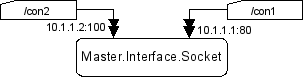
\includegraphics[scale=1]{coremod02.png}
    \caption{This figure shows the module-map of the socket-example.}
\end{figure}    
This example opens two connection to different hosts and ports:
\lstinputlisting{coremod02.py}



%
% Serial interface module:
%
\CoreModDesc{Master.Interface.UniSerial}
The \CoreMod{Master.Interface.UniSerial} core module implements the serial
interface for the PPLT system. This module needs the Python library 
\code{pySerial}. You can get this library from the URL 
\url{http://serial.sourceforge.net}. 

The settings of this module can be changed at runtime by symbols connected to
the addresses \emph{speed}, \emph{parity} \emph{timeout}.

\subsubsection{Parameters}
This module 4 parameters to setup. 
\begin{tableiii}{l|p{10cm}|l}{textrm}{Parameter}{Description}{Default value}
\lineiii{Port}
        {This is the number of the serial interface, the moudle should use. 0 
         means \code{ttyS0} or \code{COM1}, 1 means \code{ttyS1} etc. This
         parameter is not optional!}
        {---}
\lineiii{Speed}        
        {This is the speed in Baud the serial interface will be set to. This
         parameter is not optional!} 
        {---}
\lineiii{Parity}
        {This parameter specifies the parity check (settings) of the serial 
         inteface. 'Odd', 'Even', 'None' are valid values. This parameter
         is optional.}
        {'None'}
\lineiii{TimeOut}
        {This parameter sets the timeout for reading from the serial 
         interface in seconds. All floatingpoint numbers are valid an
         \code{None} means blocking-read.}
        {\code{None}}
\end{tableiii}
\notice{Some parameters can be reset at runtime by symbols connected to this 
module at special addresses. See next paragraph for details.}

\subsubsection{Addresses}
\begin{tableiii}{l|l|p{10cm}}{testrm}{Address}{Type}{Description}
\lineiii{---}
        {\code{TStream}}
        {This is the \emph{data-channel} to the serial-interface. Meaning 
         reading from this will read from the serial interface and writeing
         into a connection to this will write into the serial-interface.}
\lineiii{speed}
        {\code{TInteger}}
        {By this connector you'll be able to change the settings of the serial
         interface at runtime. Write an integer to a connection to this address
         will (try) to reset the baudrate to the value. See example for details.}
\lineiii{parity}
        {\code{TString}}
        {Writing strings like 'even', 'odd' or 'none' into this connector, will
         reset the setting of the serial interface. Reading from the connector
         will infrom you about the current setting.}
\lineiii{timeout}
        {\code{TFloat}}
        {Writing to this connector will reset the timeout for reading from 
         the serial interface.}
\end{tableiii}

\subsubsection{Example}
\begin{figure}[ht]
    \label{fig:coremod01}
    \centering
    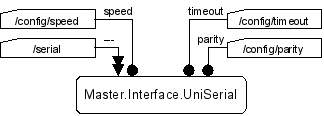
\includegraphics{coremod01.png}
    \caption{This figure shows the module-map of the UniSerial-example.}
\end{figure}    
This example shows how to setup the \CoreMod{UniSerial} and how to change the 
settings at runtime:
\lstinputlisting{coremod01.py}








%\CoreModDesc{Master.Interface.WGet}




%
% Transport layer of the Mewtocol:
%
\CoreModDesc{Master.Transport.MEWCOM-TL}
This module implements the transport-layer of the MEWTOCOL. The MEWTOCOL 
normally doesn't distinguish between the tansport and command layer. So
this module is only usfull in combination with the \CoreMod{MEWCOM-CL}
core-module that implements the command messages of the MEWTOCOL.

\subsubsection{Parameters}
This module needs only one parameter that specifies if a cecksum should
be calculated and adde to the MEWTOCOL message. By defualt this parameter
is set to \code{"True"}

\begin{tableiii}{l|p{10cm}|l}{textrm}{Parameter}{Description}{Default}
\lineiii{BCC}
        {This parameter specifies if a bcc (checksum) should be claculated
         for each packet send. This parameter doesn't contol the if the
         checksum of a recived packet will be checked. This will allways be 
         done (if the packet contains a checksum)\footnote{The MEWTOCOL 
         protocol allows that a packet doesn't contain a checksum. In this 
         case the checksum 'XX' will be set to indicate that the checksum
         should not be checked.}.  
        }{'True'}
\end{tableiii}       

\subsubsection{Addresses}
Each module or symbol have to set a address for the connection to this 
module. This address specifies the address of the destination the 
MEWTOCOL messages are send to. 
\begin{tableiii}{l|l|p{10cm}}{textrm}{Address}{Type}{Description}
\lineiii{0..255}
        {\code{TSequence}}
        {This address specifies the destination of the messages send.}
\end{tableiii}

\subsubsection{Example}
Because of this module is not usefull alone, please look at the example for 
the \CoreMod{MEWCOM-CL} core module.



%
% PPI module:
%
\CoreModDesc{Master.Transport.PPI}
This Core-Module implements the PPI protocol. It can be used to access the Siemens
SIMATIC S7 series PLCs. In this state of developing this module can't assable an
dispatch fragmentated packages. But in the most cases this is not needed. 

\subsubsection{Parameters}
This module needs only one parameter:
\begin{tableiii}{l|p{10cm}|l}{textrm}{Parameter}{Description}{Default}
\lineiii{Address}
        {This parameter specifies the PPI address of the PC. This is in the 
         most cases 0. But you have to set a value for this parameter!}
        {}
\end{tableiii}

\subsubsection{Addresses}
If you connect other modules or symbols to this module you'll need to specify
an address. This address is a number between 0 and 255. 
\begin{tableiii}{l|l|p{10cm}}{textrm}{Address}{Type}{Description}
\lineiii{0-255}{\code{Sequence}}
        {This address specifies the address of the device in the PPI BUS. 
         Writeing into the connection will cause a packet send to the device
         addressed by this address. Also reading from the connection will only
         return the content addressd to the setted Parameter \var{Address} and
         from the device addressd by this address.}
\end{tableiii}

\subsubsection{Example}
\begin{figure}[ht]
    \label{fig:coremod07}
    \centering
    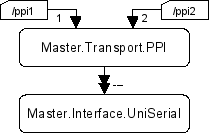
\includegraphics{coremod07.png}
    \caption{This figure shows the module-map of the PPI-example.}
\end{figure}    
This example shows how to tunnel the PPI bus by the symbol tree. For an more
usefull example please look the the Example for the \CoreMod{S7} core-module.
\lstinputlisting{coremod07.py}



%
% ReadLine module.
%
\CoreModDesc{Master.Transport.ReadLine}
This module can be used if you want to do some line-orientated communication.

This is often used for simple protocols for the serial interface. For example
the AT commands for modems but also the Mewtocol by Panasonic (FP0 and FP1) 
uses a line-orientated protocol to send or recive commands to/from the PLC.  

So this module have to be used as a child of a module that provides
\code{TStream} or \code{TSequence} connections.

\subsubsection{Parameters}
This module needs a parameter to specify the \emph{line-end} character(s).
\begin{tableiii}{l|p{10cm}|l}{textrm}{Paramter}{Description}{Default}
\lineiii{LineEnd}
        {A hex-encoded string that the module will use as a sign for the 
         line-end. And also all data send over this module will be extended
         with this string.}
        {0A0D} 
\end{tableiii}

\subsubsection{Addresses}
This module knows only one address: no address.
\begin{tableiii}{l|l|p{10cm}}{textrm}{Address}{Type}{Description}
\lineiii{---}
        {\code{TSequence}}
        {All data written into this connector will be extended by the set 
         line-end. And also if you read from this connector it will block 
         until the set line-end character(s) appear in the data-stream.
         \textbf{Note:} The whole line will be then returned!}
\end{tableiii}

\subsubsection{Example}
\begin{figure}[ht]
    \label{fig:coremod10}
    \centering
    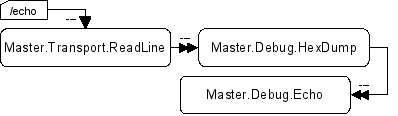
\includegraphics{coremod10.png}
    \caption{This figure shows the module-map of the ReadLine-example.}
\end{figure}    
This example shows on the one hand the usage of the \CoreMod{ReadLine} module.
On the other hand it is a quite good test for the \CoreMod{Echo} module. 
This example write a string into \CoreMod{ReadLine} that extends the string 
with the line-end. Then it will send this message to the \CoreMod{Echo} module.
Then it trys to read from \CoreMod{ReadLine} that trys to read a complete 
line from his parent (\CoreMod{Echo}) strips the line-end characters and
return the string. If all goes well the same string will be returned. To see
what's going on a \CoreMod{HexDump} module will be plugged between the 
\CoreMod{Echo} and \CoreMod{ReadLine} modules.
\lstinputlisting{coremod10.py}



%
% Agilent 5462x series oscilloscopes 
%
\CoreModDesc{Master.Device.5462X}
This module implements the command messages to access an Agilent 
oscilloscopes. This module only supports the message format used 
by the serial interface of the oscilloscope. So you need to connect
this module (indirect) to the \CoreMod{Master.Interface.UniSerial}
core-module.

\subsubsection{Parameters}
This module need two parameters to be set up. These parameters specify the
primary and secondary signal source. If you only want to use the primary
source you should set the secondary to the same source like the primary.
\begin{tableiii}{l|p{10}|l}{textrm}{Parameter}{Description}{Default}
\lineiii{PSource}
        {This specifies the primary source. This can be one of A0 (analog \#1),
         A1 (analog \#2), M (math) or F (form).}{---}
\lineiii{SSource}
        {This specifies the secondaray source. Look at \var{PSource} for more
         details}{---}
\end{tableiii}         
\bf{To be continued}\bf{To be continued}

%
% Panasonic A200 Imagechecker
%
%\CoreModDesc{Master.Device.A200}



%
% GSM compatible mobile-phone.
%
\CoreModDesc{Master.Device.GSM}



%
% Command-messages for the Panasonic FP0 and FP1
%
\CoreModDesc{Master.Device.MEWCOM-CL}
This core-module implements the command messages of the MEWTOCOL. This 
protocol is used to access the Panasonic FP0 FP2 PLCs. So you can access
the markers of these PLCs using the \CoreMod{Master.Transport.MEWCOM-TL},
\CoreMod{Master.Device.MEWCOM-CL} core-modules and a interface module like 
\CoreMod{Master.Interface.UniSerial} or \CoreMod{Master.Interface.Socket}.

\subsubsection{Parameters}
This module needs no parameters to be set up.

\subsubsection{Addresses}
You have to set a address to connect a symbol to this module! With this 
address you specify the marker you want to get/set. Additional there is a
address called \code{"STATUS"} that controls the state of the PLC 
(\emph{run}/\emph{stop}).
\begin{tableiii}{l|p{2cm}|p{10cm}}{textrm}{Address}{Type}{Description}
\lineiii{STATUS}
        {\code{TBool}}
        {By this address you can control the state of the PLC. If it is 
         \code{True} then the PLC is in the \emph{Run} mode. You can also
         get the state of the PLC by reading this value.}
\lineiii{\emph{Marker}}
        {\code{TBool} or
         \code{TInteger}}
        {By setting a marker-address as the address for the connection to this 
         module, you are able to access (read/write) this marker. So the type 
         of the connection you'll get depends on the marker-address you set.} 
\end{tableiii}

\subsubsection{Example}
\begin{figure}[ht]
    \label{fig:coremod11}
    \centering
    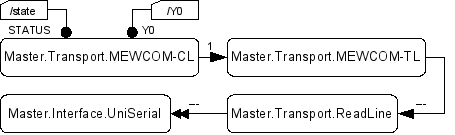
\includegraphics{coremod11.png}
    \caption{This figure shows the module-map of the MEWCOM-CL example.}
\end{figure}    
This example shows how to access a FPx using the \emph{ToolPort} (serial interface).

\lstinputlisting{coremod11.py}



%
%
%
\CoreModDesc{Master.Device.S7}
This module implements the command-messages of the Siemens SIMATIC S7(-200). 
With this module and the \CoreMod{Master.Transport.PPI} and 
\CoreMod{Master.Interface.UniSerial} it is possible to access the S7 over the 
PPI bus. To do this you must configure the serial interface in a special way. 
Look at the example to find out how. This module can generate messages that 
cause the S7 to send the value of the requested marker. To specify the marker 
you want to get you have to connect a symbol with this module with the name of
the marker as address. It could be possible that not all availabe marker can be
read. If you know some of them please let me know.

\subsubsection{Parameters}
This module needs no parameters to be set up.

\subsubsection{Addresses}
The address you have to specify to connect a symbol to this module should be 
the name of the marker you want to get/set.
\begin{tableiii}{l|p{2cm}|p{10cm}}{textrm}{Address}{Type}{Description}
\lineiii{\emph{Marker}}
        {\code{TBool}, \code{TInteger}}
        {With the address you specify the marker you'll access. So the type 
         of the values you'll get depends on the marker you'll set. So if you 
         access an boolean marker you'll get values typed \code{TBool} if you
         access byte,word and double word Markers you'll get values types
         \code{TInteger}.}
\end{tableiii}

\subsubsection{Example}
\begin{figure}[ht]
    \label{fig:coremod08}
    \centering
    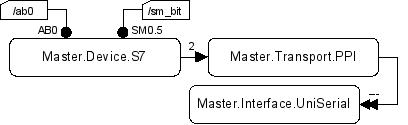
\includegraphics{coremod08.png}
    \caption{This figure shows the module-map of the S7-example.}
\end{figure}    
In this example I'll access (read/write) the markers SM0.5 (special marker 0 bit 5) and AB0
(output byte 0).

\lstinputlisting{coremod08.py}



%
% ECHO module
%
\CoreModDesc{Master.Debug.Echo}
This module echoes all data writte to it at reading from it. It can be used to
debug other modules. This is a so called \emph{root}-module. It can't be 
loaded as a child of an other module!

\subsubsection{Parameters}
This module needs no parameters!

\subsubsection{Addresses}
This module has only one addresses: no address.
\begin{tableiii}{l|l|p{10cm}}{textrm}{Address}{Type}{Description}
\lineiii{---}
        {\code{TStream}}
        {If you write into a symbol connected to this module, the data will be
         buffered and the next time you read from it the buffer (or a part of 
         it) will be returned.}
\end{tableiii}

\subsubsection{Example}
\begin{figure}[ht]
    \label{coremod06}
    \centering
    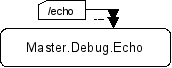
\includegraphics{coremod06.png}
    \caption{This figure shows the module-map of the Echo-example.}
\end{figure}    
This is a simple echo-example... ... the classic.

\lstinputlisting{coremod06.py}



%
% HexDump Module 
%
\CoreModDesc{Master.Debug.HexDump}
This module is a simple trafic dumper. It dumps all data going throught it
into the logging-system with loglevel \emph{debug}. So you can read it from
your logfile or \code{stderr}. Simply plug this module between two modules
to record all trafic.

\subsubsection{Parameters}
This module needs no parameters!

\subsubsection{Addresses}
This module has only one address: no address! 
\begin{tableiii}{l|p{2cm}|p{10cm}}{textrm}{Address}{Type}{Description}
\lineiii{---}
        {\code{TStream} or \code{TSequence}}
        {All data written to this module will be written to the parent and 
         read vica versa. So the type of the connection will depend on the
         type of the parent-connection.}
\end{tableiii}

\subsubsection{Example}
\begin{figure}[ht]
    \label{fig:coremod05.py}
    \centering
    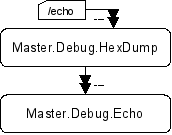
\includegraphics{coremod05.png}
    \caption{This figure shows the module-map of the HexDump-example.}
\end{figure}    
This module uses the echo module to show how the trafic in read and write 
direction will be dumped:
\lstinputlisting{coremod05.py}



%
% Null module (the black hole)
%
\CoreModDesc{Master.Debug.Null}
This is a very simple module, that works like the /dev/null device file on 
Linux. If you read from this module, you'll get a string with zero-bits and
if you write into this module nothing will happens. This module swallow all
you write into it.

\subsubsection{Parameters}
This module needs no parameters to be set up.

\subsubsection{Addresses}
This module has only one valid address: no address.
\begin{tableiii}{l|l|p{10cm}}{textrm}{Address}{Type}{Description}
\lineiii{---}
        {\code{TStream}}
        {This will be the connection to the \CoreMod{Null} module. Id you
         write into this connection the module will swallow all data and
         nothing will happen. If you read from this module you'll get a 
         stream of zero-bits.}
\end{tableiii}

\subsubsection{Example}
\begin{figure}[ht]
    \label{fig:coremod09}
    \centering
    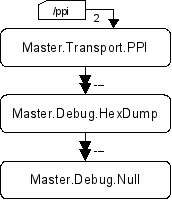
\includegraphics{coremod09.png}
    \caption{This figure shows the module-map of the Null-Example.}
\end{figure}    
This example shows a configuration to debug a non \emph{root} module. In this 
case it is the \CoreMod{Master.Transport.PPI} core-module. To get some 
information about the packages the PPI module sends the core-module 
\CoreMod{Master.Debug.HexDump} is used.  \notice{This example raises an 
exception, because the PPI module expect a correct answer from the 
\emph{virtual} device (in this case the core-module 
\CoreMod{Master.Debug.Null}).
\lstinputlisting{coremod09.py}



%
% Random-generator module
%
\CoreModDesc{Master.Debug.Random}
This module implements a random-generator, that can generate data for every 
symbol-type supported by the \module{pyDCPU}. So this module can be used to 
test almost all facilities of the system. 

\subsubsection{Parameters}
This module needs no parameters. 

\subsubsection{Addresses}
\begin{tableiii}{l|l|p{10cm}}{testrm}{Address}{Type}{Description}
\lineiii{Bool}
        {\code{TBool}}
        {Provide a random boolean value.}
\lineiii{Integer}
        {\code{TInteger}}
        {Provide a random integer value between 0 and 100.}
\lineiii{Float}
        {\code{TFloat}}
        {Provide a random floating point number between 0 and 1.}
\lineiii{String}
        {\code{TString}}
        {Provide a random string of a random length between 1 and 79 containg 
         printable characters.}
\lineiii{ArrayBool}
        {\code{TArrayOfBool}}
        {The name tells everything. The length of the array is randomly 
         between 1 and 3.}
\lineiii{ArrayInteger}
        {\code{TArrayOfInteger}}
        {Array of integer of random length between 1 and 3.}
\lineiii{ArrayFloat}
        {\code{TArrayOfFloat}}
        {Array of floating point numbers with variable length between 1 and 
         3.}
\lineiii{ArrayString}
        {\code{TArrayOfString}}
        {Array of string with variable length (of array) between 1 and 3.}
\lineiii{Stream}
        {\code{TStream}}
        {Provides an random data string. The data are printable character.
         The number of bytes returned is less than equeal the number you 
         wanted to read. To read from a symbol connected to this address,
         please use the method \method{SymbolTreeRead().}}
\lineiii{Sequence}
        {\code{TSequence}}
        {A sequence of random data. The data contains only printable 
         characters and the length varies between 1 and 79.}
\end{tableiii}

\subsubsection{Example}
This is a simple example that uses all types:
\lstinputlisting{coremod03.py}



%
% Statistic module
%
\CoreModDesc{Master.Debug.Statistic}
This module collects statistical values of the data flowing through it. You 
can use this module to improve or debug your own modules or even to observe
the PPLT system. This module is quite easy to use: simply plug this between 
two other modules and you are able to observe the trafic between them.
\notice{You can only observe modules that provides a \code{TStream} or 
\code {TSequence} connection.}

\subsubsection{Parameters}
This module needs no parameters!

\subsubsection{Addresses}
There are several addresses provideing the statistical data. If you use no 
address to connect to this module a \code{TStream} or \code{TSequence} 
connection to the parent will be returned. This connection to the parent will
be used to collect the statistical data. 

\begin{tableiii}{l|p{2cm}|p{10cm}}{textrm}{Address}{Type}{Description}
\lineiii{---}
        {\code{TStream} or \code{TSequence}}
        {This is the data-tunnel to the parent of the 
         \CoreMod{Statistic}-module. The type of the connection depends on
         the type of the connection to the parent module. You see, it is only
         possible to connect the \CoreMod{Statistic}-module to a parent that
         provides a \code{TStream} or \code{TSequence} connection.}
\lineiii{read\_data}
        {\code{TInteger}}
        {Returns the number of bytes read from the parent.}
\lineiii{write\_data}
        {\code{TInteger}}
        {Returns the number of bytes written to the parent.}
\lineiii{read\_speed}
        {\code{TFloat}}
        {Returns the number of bytes per second read from parent since 
         module-loading. This value is the average of the whole time since
         module-loading.}
\lineiii{write\_speed}
        {\code{TFloat}}
        {Returns the number of bytes written to the parent since the module 
        was loaded. This value is the average of the whole time.}
\lineiii{error}
        {\code{TInteger}}
        {Returns the number of read/write-errors since the module was loaded.
         This must not be an indicatior for bugs in the parent modules because
         also timeouts will be recorded.}
\end{tableiii}

\subsubsection{Example}
In this example the serial interface will be exported by the symbol tree.
The \CoreMod{Statistic}-module records the trafic throught the serial 
interface.
\lstinputlisting{coremod04.py}



\newpage
\section{Export modules}
\CoreModDesc{Export.JVisu}
\CoreModDesc{Export.SimpleExport}
\CoreModDesc{Export.PPLTWeb}


%    \chapter{How to write Core modules}

    
    \newcommand{\PSFTag}[1]{\index{PSF Elements!#1}}



\chapter{PSF Reference --- \textbf{P}PLT \textbf{S}ession \textbf{F}ile}

This section describes the file-format of the PPLT session files. Such 
files contain the information about the state of the system. 
So the file contains information about the loaded devices and servers and
also the layout of the symbol-tree.

Files formatted in the PSF format can be created from a running PPLT system by 
a call of the method \method{SaveSession()} and can then be loaded by a 
\method{LoadSession()} method-call.

By this way you can easily implement a simple daemon or service, that reads 
such a PSF file and setup a whole PPLT system. Meaning loading all devices, 
creating all symbols and folders and at the end loading all servers.

All you need to know is a basic knowledge of XML formats, and a little idea of 
what PPLT is and what the system needs to save (or even needs to know to setup
the PPLT system). 

\section{Reference}
In the following section I'll list all keyword of the PSF format. These are only few
because the format stills easy. 

At first: The PSF format is an XML format!

\subsection{\keyword{PPLTSession}}
\PSFTag{PPLTSession}
The PPLTSession tags surround the PPLT session document. Containing all 
information about the devices, servers and symbol-tree. This tag must
(directly) contain the elements (tags) \keyword{Servers}, \keyword{Devices}
and \keyword{SymbolTree}. But each elements can only occur once.
This also defines the basic layout of the PPLT session document. Each document
should look like:
\begin{verbatim}
<?xml version="1.0"?>
<PPLTSession>
    <Servers>
        [...]
    </Servers>
    <Devices>
        [...]
    </Devices>
    <SymbolTree>
        [...]
    </SymbolTree>
</PPLTSession>
\end{verbatim}


\subsection{\keyword{Servers}}
\PSFTag{Servers}
The tag \keyword{Servers} contains the description of all loaded servers. This tag can only 
contain any occurrence of the tag \keyword{Server}. Each \keyword{Server}-tag describe a 
singe server to load. For more details see at the description of the \keyword{Server}-tag.

\begin{verbatim}
[...]
    <Servers>
        <Server [...]>
            [...]
        </Server>
        [...]
    </Servers>
[...]
\end{verbatim}


\subsection{\keyword{Server}}
\PSFTag{Server}
The tag \keyword{Server} describes a server to load. The tag can only contain any occurrence of the tag
\keyword{Parameter}. Each \keyword{Parameter} tag specifies a parameter needed to load the server.
Also the \keyword{Server} needs some attributes. The attribute \var{alias} specifies the alias the
server will get after it was loaded. The attribute \var{fqsn} specifies the full-qualified-server-name. 
This unique name specifies the server to be loaded. The Attribute \var{root} specifies the server root.
\note{The given server-root but exist else the loading of the server will fail.} The attribute 
\var{user} specifies the default user. The server will run with the rights of this user, if the 
server doesn't know any authentication. 

A simple example will can be:
\begin{verbatim}
[...]
    <Server alias="JVisu" fqsn="Visu.JVisuServer" root="/" user="admin">
        <Parameter name="Port">2200</Parameter>
        <Parameter name="Address">127.0.0.1</Parameter>
    </Server>
[...]
\end{verbatim}
This example will start a JVisu server with the rights of the user \code{admin} and
with the server root \code{'/'}. JVisu is a open source visualization written in Java.
You can get it from \url{http://jvisu.sourceforge.net}.

\subsection{\keyword{Parameter}}
\PSFTag{Parameter}
The \keyword{Parameter}-tag specifies a parameter, the system will use to setup
a \keyword{Server} or \keyword{Device}. The \keyword{Parameter}-tag can only 
contain CDATA, meaning it can only contain a string. The content will be 
interpreted as the value of the parameter. The \keyword{Parameter}-tag
knows also a attribute. The attribute \var{name} specifies the name
of the parameter. To find out what parameters are needed to setup
a specific server, please consult the Device and Server reference.


\subsection{\keyword{Devices}}
\PSFTag{Devices}
Like the \keyword{Servers}-tag this tag contains the description of
all devices needed to be loaded. So this tag can only contain any
occurrence of the tag \keyword{Device}. For example:
\begin{verbatim}
[...]
    <Devices>
        <Device [...]>
            [...]
        </Device>
        [...]
    </Devices>
[...]
\end{verbatim}


\subsection{\keyword{Device}}
\PSFTag{Device}
Like the \keyword{Server}-tag this tag describes one device to load. Also it can only contain 
any number of \keyword{Parameter} tags to specify the the parameters the device may need to be
loaded. It also has some attributes. The attribute \var{alias} specifies the alias the device 
gets when it's was successfully loaded. The attribute \var{fqdn} specifies the full qualified 
device name. This is the name of the device you want to load.

For example, a \keyword{Devices}-section can be:
\begin{verbatim}
[...]
    <Devices>
        <Device alias="rand" fqdn="Debug.RandomGenerator"/>
        <Device alias="S7" fqdn="PLC.S7-200">
            <Parameter name="PCAddr">0</Parameter>
            <Parameter name="Port">1</Parameter>
            <Parameter name="S7Addr">2</Parameter>
        </Device>
    </Devices>
[...]
\end{verbatim}
This example will load a random-generator as \code{'rand'}  and the support for the Siemens SIMATIC S7-200 
as \code{'S7'}.


\subsection{\keyword{SymbolTree}}
\PSFTag{SymbolTree}
The \keyword{SymbolTree}-section describes the content of the symbol-tree. So this tag can only contain
any occurrence of \keyword{Symbol} and \keyword{Folder} tags. This tag don't take any attributes.

\subsubsection{How the symbol-tree is depicted}
The symbol-tree works like a small filesystem, with folders, sub-folder and symbols. The root of this filesystem is the
symbol-tree itself. Now you need to know how to depict the hierarchy of the symbol-tree to an XML file.

I think the best way to describe is to give an example. The following symbol-tree hierarchy
\begin{verbatim}
/
/FOLDER1/
/FOLDER1/FOLDER2/
/FOLDER1/FOLDER2/Symbol1
/FOLDER1/FOLDER2/Symbol2
/FOLDER1/Symbol3
/FOLDER3/
/FOLDER3/Symbol4
/Symbol5
\end{verbatim}
will be depicted as something like:
\begin{verbatim}
<SymbolTree>
    <Folder name="FOLDER1">
        <Folder name="FOLDER2">
            <Symbol name="Symbol1"/>
            <Symbol name="Symbol2"/>
        </Folder>
        <Symbol name="Symbol3"/>
    </Folder>    
    <Folder name="FOLDER3">
        <Symbol name="Symbol4"/>
    </Folder>
    <Symbol name="Symbol5"/>
</SymbolTree>
\end{verbatim}
As you see; the \keyword{SymbolTree} can contain \keyword{Symbol}s and \keyword{Folder}s. And each \keyword{Folder} can
also contain \keyword{Symbol}s and \keyword{Folder}s. But only the \keyword{Symbol}s are empty, because they can't contain
anything. In this example I missed some additional attributes to avoid you to be confused. This attributes are described 
in detail in the following sections.

\subsection{\keyword{Symbol}}
\PSFTag{Symbol}
The \keyword{Symbol}-tag describes a symbol of the symbol-tree. Such a symbol is a kind of a variable that can hold values.
Each symbol is connected to a so called "symbol-slot"\footnote{A symbol-slot always belongs to a device, so if you want to know 
what slots are provided by a specific device, pleas look at the documentation of the device.}. So you need to specify the 
symbol-slot the symbol will be connected to by the attribute \var{slot}. The slot-name must be provided in the format 
\code{'DEVICE\_ALIAS::NAMESPACE::SLOT\_NAME'}. The \code{DEVICE\_ALIAS} specifies the device you want the symbol to be
connected to. It should be the string you give to the \keyword{Device}-attribute \var{alias}. The \code{NAMESPACE}s and
\code{SLOT\_NAME}s are provided by the devices. To find out what namespaces are available, look at the documentation of 
each device.

In this context you also need to define the type of the symbol by the attribute \var{type}. The type is defined by the
slot you use. So please take a look at the documentation of the specific device.

Now your symbol can get and (maybe) set values. But a major feature of the PPLT is, that you can control the
access to the symbol by setting rights to it. To do so, you need to set a \var{owner}, \var{group} and
\var{modus} to the symbol (and also to the folder). So a complete example for a symbol that is connected to
a random-generator loaded as \code{'rand'} could be:
\begin{verbatim}
[...]
    <SymbolTree>
        <Symbol name="r_bool" slot="rand::Generator::Bool" type="Bool" 
                owner="admin" group="Admin" modus="600"/>
        [...]
    </SymbolTree>
[...]
\end{verbatim}
You see the attribute \var{modus} contains a 3-digit integer. This integer is calculated like the Linux modus integer. Pleas look
at the \manpage{chmod}{} man-page to get more information. But sofar the number \code{600} says that only the owner has the right to 
read/write to the symbol and the group and any other has no rights.


\subsection{\keyword{Folder}}
\PSFTag{Folder}
The \keyword{Folder}-tag describes a folder in the symbol-tree. The name of the folder will be specified by the
attribute \var{name}. Like the symbols a folder also owned by a user and attached to a group. So you also need 
to set the \var{owner}, \var{group} and \var{modus} attributes. 

\newpage
\section{A complete Example}
In the following section I'll show you a complete example of a PSF. The file describes two devices, a random generator and
a Siemens SIMATIC S7-200. The symbol-tree contains two folders one, named 'Rand', will contain some symbols connected
to the random-generator and the other, named 'S7' will contains the symbols connected to the S7. And a web-server will be loaded, 
that exports the whole symbol-tree. 

\verbatiminput{PSF.xml}



    
    \documentclass{manual}

\title{PPLT References}
\author{Hannes Matuschek\\\texttt{<hmatuschek@gmx.net>}}
%\date{2005-10-12}
\release{0.9.0}
\setshortversion{0.9.0(beta)}
\makeindex


 \begin{document}
   
    \maketitle
    \begin{abstract}
    This document summarize the references of the PPLT system. Including Core-Library reference, reference
    of the PPLT abstraction layer, documenttypes and some other stuff.
    \end{abstract}

    \tableofcontents


    \chapter{PPLT Reference}
\section{\module{PPLT} ---
        \textbf{P}otsdamer \textbf{P}rozess \textbf{L}eit \textbf{T}echnik}

\declaremodule{}{PPLT}
\moduleauthor{Hannes Matuschek}{hmatuschek@gmx.net}
\modulesynopsis{The PPLT is a framework for master/slave based communication.}

The \module{PPLT} builds an abstraction layer over the core library 
(\module{pyDCPU}). With the PPLT you can easily handle abstract devices and 
server instead of handle with several core modules. Like the core-library the 
PPLT has only one class called \code{System}. After instancing this class, all
work can be done by calling the methods of this object.

\section{Class description}
\begin{classdesc}{System}{\optional{BasePath}, \optional{CoreLogLevel}, 
\optional{PPLTLogLevel}, \optional{LogFile}, \optional{Syslog}, 
\optional{Lang}, \optional{AltLang}}
This is the all-in-one class. If this class will be instanced the complete 
PPLT system will be loaded. Meaning searching plug-ins (modules), loading 
user-database, starting core-system, etc...

The argument \var{BasePath} specifies the path of all PPLT related stuff. This 
is by default \code{sys.exec\_prefix+'/PPLT'}. Under Windows this is the folder 
where you've installed Python under \UNIX this should be some thing like 
\code{/usr/local/PPLT}. If you miss this argument, the default path will be 
used.

The argument \var{CoreLogLevel} specifies the log-level for the core library. 
This should be one of \code{off}, \code{fatal}, \code{error}, \code{warning}, 
\code{info}, \code{debug}.  If you select \code{debug} a lot of (not always 
useful) messages will be logged and \code{off} switches the logging off. 
By default the logging level \code{info} will be used. If you miss this 
argument, the default value will be used.

The argument \var{PPLTLogLevel} specifies the log-level of the PPLT library. 
This should be one of \code{off}, \code{fatal}, \code{error}, \code{warning}, 
\code{info}, \code{debug}. If you select \code{debug} a lot of (not always 
useful) messages will be logged and \code{off} switches the logging off. 
By default the logging level \code{info} will be used. If you miss this 
argument, the default value will be used.

The argument \var{LogFile} specifies the file,  where the logging messages are
written to. If you missed this argument, there were no messages written to any
file, all messages were send to screen (\code{stderr}). 

The boolean argument \var{SysLog} specifies if the messages should be send to
the local \code{syslog}-daemon. 
\begin{notice}
This argument overwrites the optional argument \var{LogFile}. If \var{SysLog}
it \code{True} no messages were written into any file nor send to screen!
\end{notice}
By default this argument if \code{False}. If you missed this argument, the 
default will be used.

The argument \var{Lang} specifies the primary language the system will use for
module description. This option do not change the language of the logging 
messages (they are not translated). This option is not important for normal
usage of the PPLT. By default \code{'en'} will be used.

The argument \var{AltLang} specifies the alternative language to be used
for module description. This should be always \code{'en'}. \textbf{Do not 
change until you know what you do.} 

If the primary language can not be found, the alternative will be used. 
\end{classdesc}




\section{Methods of \class{System}}
In this section I will describe the methods of the \class{System}-class. I 
will not list all available methods, because there are more then 60 of it. Some
of them are only useful if you want to write a GUI application like the
\emph{PPLT Center}. But you can get a short help over all methods by calling
\code{pydoc PPLT.System}. 


\subsection{Device methods}
\begin{methoddesc}[System]{LoadDevice}{DeviceName, Alias, Parameters}
This is one of the most important methods. With this method you can load and
setup a device. This method loads the device \var{DeviceName} as \var{Alias}. 
The alias will be used later to specify this device, for example if you want
to connect a symbol to this device or unload the device.

The argument \var{DeviceName} specifies the full qualified device name. All
devices (and servers) are grouped by classes. A full qualified device name
consists always of all classes and the name divided by a single dot. For
example \code{'PLC.Panasonic-FPX'}.

The argument \var{Alias} specifies the alias the device will get after being
loaded. By this alias you will identify the device later.

The attribute \var{Parameters} specifies the parameters the device needs to be
set up successfully. This should be a dict with key-value pairs. The key 
is the parameter name and the value should be the parameter-value. For example:
\code{\{'Port':'0', 'Address':'123'\}}.
\begin{notice}
All parameter names and also \textbf{all} parameter values are strings!
\end{notice}

This method will return \code{Ture} on success an \code{False} on error.
\end{methoddesc}


\begin{methoddesc}[System]{UnLoadDevice}{Alias}
This method unload and destroy the given device. 

The argument \var{Alias} specifies the alias of the device you want to be
unloaded. This is the alias you've set at the \method{LoadDevice} 
method-call.

This method returns \code{True} on success and \code{False} on error.
\end{methoddesc}


\begin{methoddesc}[System]{GetFQDeviceName}{Alias}
This method returns the full qualified device name of the device loaded as
\var{Alias}.

The attribute \var{Alias} specifies the alias of the loaded device. This is
the alias you've set at the \method{LoadDevice} method-call.

This method returns a string containing the full qualified device name or non 
if the alias if not a device or not loaded.
\end{methoddesc}


\begin{methoddesc}[System]{GetDeviceParameters}{Alias}
This method will return the parameters the device was loaded with. This method
will return a dict on success or \code{None} on error.
\end{methoddesc}


\subsection{Server methods}
This section describes all methods to handle servers, like starting, stopping, ... 

\begin{methoddesc}[System]{LoadServer}{ServerName, Alias, DefaultUser, Parameters\optional{, Root}}
This method loads and setup a server. 

The argument \var{ServerName} specifies the full qualified server name. Full 
qualified means that all classes and the name are given, divided by a single 
dot (like: \code{Web.PPLTWebServer}).

The argument \var{Alias} specifies the alias the server will have after 
being loaded. By this alias you will identify the server later, for example 
to unload this server.

The argument \var{DefaultUser} specifies the the user, the server will run as. 
By this option you can assign rights to a server, that doesn't know any 
authentication. By default, a server should support a authentication but 
sometimes the used protocol doesn't (for example JVisu). For this kind of 
server this option is useful.

The argument \var{Parameters} specifies the parameters the server will be 
loaded with. This should be a dict with the parameter name as key (string)
and the parameter value as value (also a string!). If a server doesn't needs
any parameters, please set \var{Parameters} to \code{None} or to and empty 
dict (\code{\{\}}). 

The optional argument \var{Root} specifies the server-root of this server. 
By default (\var{Root}=\code{'/'}) the whole symbol-tree will be accessible
by this server. But if you want to export only a specific folder of the 
symbol-tree you can specify this folder with the \var{Root} argument. So
if \var{Root}=\code{'/test'} only the content of the folder \code{'/test'}
will be accessible by this server.

This method returns \code{True} on success and \code{False} else.
\end{methoddesc}


\begin{methoddesc}[System]{UnLoadServer}{Alias}
This method will stop and destroy a server loaded with \method{LoadServer}.

The attribute \var{Alias} specifies the server you want to stop. This is the 
alias you've defined on loading the server with \method{LoadServer}.

This method will return \code{True} on success and \code{False} else.
\end{methoddesc}


\begin{methoddesc}[System]{GetFQServerName}{Alias}
This method will return the full qualified server-name of the loaded server
by his alias. 

The argument \var{Alias} specifies the alias of the server. This is the alias
you have defined on loading by the \method{LoadServer} method.

This method returns a string on success or \code{None} on error.
\end{methoddesc}


\begin{methoddesc}[System]{GetServerParameters}{Alias}
This method will return the dict of parameters the server was loaded with. 
This is the parameter dict, you have defined on loading the server with 
\method{LoadServer}.

The argument \var{Alias} specifies the alias of the loaded server. This is
the alias you have defined on loading the server with \method{LoadServer}.

This method will return a dict or \code{None} on error. This method will
return an empty dict even if you've loaded the server with no parameters.
\end{methoddesc}


\begin{methoddesc}[System]{GetServerRoot}{Alias}
This method will return the server root of a loaded server. This is the 
server root you have defined on loading the server with \method{LoadServer}.

The server root is the base folder in the symbol-tree the server can access. 
Only folders and symbols laying under this folder are accessible by this 
server.

The argument \var{Alias} specifies the alias of the loaded server. This is the
alias you have defined on loading the server with \method{LoadServer}. 

This method will return a string on success or \code{None} on error.
\end{methoddesc}


\begin{methoddesc}[System]{GetServerDefaultUser}{Alias}
This method will return the default-user the server is running with. This is
the username you have defined on loading the server with \method{LoadServer}.

If specified, the server will run with the rights of the default user. This is
necessary, because there are some servers which don't know any authentication!

The argument \var{Alias} specifies the alias of the loaded server. This is the 
alias you have defined for this server on loading with \method{LoadServer} 
call.

This method will return a string on success or \code{None} on error.
\end{methoddesc}


\subsection{Symboltree methods}
In the following section I will describe all methods for handling the symbol-tree. 
Like creating folder and symbols, moving them, ...

All methods, that working with the access-rights of a symbol or folder
are using following scheme to encode the rights:

\begin{center}
\begin{tabular}{|c|cc||c|cc||c|cc|} \hline\hline
\bf{Own} & $r$&$\not r$&\bf{Grp}&$r$ & $\not r$ & \bf{Any} & $r$ & $\not r$\\\hline
$w$ & 6 & 2 & - & 6 & 2 & - & 6 & 2 \\
$\not w$ & 4 & 0 & - & 4 & 0 & - & 4 & 0 \\\hline\hline
\end{tabular}
\end{center}
The access-right is represented as a string of 3 numbers each number specifies 
a access right. The first number specifies the right of the owner of the 
symbol or folder. The second specifies the right of the group assigned to the 
symbol/folder.  The last number specifies the right of everyone who not 
belongs to the assigned group nor being the owner. To en/decode the 
representation you can use the table above.


\begin{methoddesc}[System]{CreateFolder}{Path\optional{, Modus}\optional{, Owner}\optional{, Group}}
This method will crate a new folder (at \var{Path}) at the symbol-tree. 
Optional you can set the rights of this folder by the arguments \var{Modus}, 
\var{Owner}, \var{Group}. If the folder was successfully created, the method 
returns \code{True} else it returns \code{False}.

The argument \var{Path} specifies the \textbf{complete} path of the folder, 
you want to create. You cant create folders relative to an other because the 
system don't know the relative.

The argument \var{Modus} specifies the modus the folder will have. By this 
argument you can set the access rights of this folder. The argument should be
a string with an octal integer in it. Meaning something like this: \code{'600'}.
Each number of the integer represents the encoded right. For the owner of the
folder (1st number), the group assigned to the folder (2nd number), and any other
(last number). For encoding you can use table above. 
By default the modus will be \code{'600'}. This denotes that only the owner 
of the folder have read/write access. (By default this will be the system admin.)

The argument \var{Owner} specifies the owner of the folder. This have to be 
existing user-name. 

The argument \var{Group} specifies the group, the folder will be assigned to. 
This have to be an existing group-name.

\begin{notice}
You can reset the modus, owner and group later by calling 
\method{ChangeModus}, \method{ChangeOwner} or \method{ChangeGroup}.
\end{notice}
\end{methoddesc}


\begin{methoddesc}[System]{DeleteFolder}{Path}
With this method you can delete an \textbf{empty} folder of the symbol-tree.

The argument \var{Path} specifies the \textbf{full} path to the folder you want to
delete. This is the path you've set on create the folder by 
\method{CreateFolder} method-call.

This method returns \code{True} on success an \code{False} else.
\end{methoddesc}


\begin{methoddesc}[System]{MoveFolder}{From, To}
This method moves a folder to an other or to the root of the symbol-tree.

The argument \var{From} specifies the \textbf{full} path of the folder you want
to move. The argument \var{To} specifies the \textbf{full} path of the destination 
folder you want the source folder to be moved to. Of cause, the destination folder
can't be a sub-folder of the source.

This method returns \code{True} on success an \code{False} on error.
\end{methoddesc}


\begin{methoddesc}[System]{ListFolders}{Path}
This method returns the names of all folders in \var{Path}.

The argument \var{Path} specifies the \textbf{full} path of the parent-folder
you want to list it's sub-folders. If you want to list the root path, please 
set \var{Path}=\code{'/'}.

The method returns a list of strings on success or \code{None} on error. 
This method will return an empty list if the given folder doesn't contain 
any sub-folders.
\end{methoddesc}


\begin{methoddesc}[System]{CreateSymbol}{Path, Slot, Type, \optional{, Modus}\optional{, Owner}\optional{, Group}}
This method creates a new symbol on path \var{Path} connected to the slot \var{Slot} and associated with the type
\var{Type}. Optional you can set the owner, group and access rights of the new symbol.

The argument \var{Path} specifies the full path to the symbol that should be 
created. \textbf{Note}: All folder on this path must exist! 

The argument \var{Slot} specifies the full qualified slot name of the slot you
want the symbol to be connected to. Thy typical format of a slot-name is 
\code{DEVICEALIAS::NAMESPACE::SLOT}. Please substitute the alias of the device
the symbol will be attached to with \code{DEVICEALIAS}. You can find the 
namespaces and slot/slot-ranges the device provide at the Chapter 
\emph{PPLT Modules}.

The argument \var{Type} specifies the type-name the symbol will associated 
with. This should be one of \code{'Bool'}, \code{'Integer'}, 
\code{'uInteger'}, \code{'Float'}, \code{'Double'}, \code{'String'}, 
\code{'ArrayOfBool'}, \code{'ArrayOfInteger'}, \code{'ArrayOfuInteger'},
\code{'ArrayOfFloat'}, \code{'ArrayOfDouble'}, \code{'ArrayOfString'} and
\code{'Raw'}.

The optional argument \var{Modus} specifies the access-right of the new symbol.
This should be a string (i.e. \code{'600'}) containing an octal integer 
representing the access-rights like described above.

The optional argument \var{Owner} specifies the owner of the symbol. This
should be a string containing a existing user-name. By default this will be
the user marked as super-user.

The optional argument \var{Group} specifies the group, the symbol will be 
attached to. This should be a string containing the name of an existing 
group. By default this will be the group of the super-user.

This method will return \code{True} on success or \code{False} else.
\end{methoddesc}


\begin{methoddesc}[System]{DeleteSymbol}{Path}
This method will remove a symbol from the symbol tree.

The argument \var{Path} specifies the \textbf{full} path
to the symbol you want to remove. 

This method will return \code{False} on error or \code{True} on success.
\end{methoddesc}


\begin{methoddesc}[System]{MoveSymbol}{From, To}
This method moves a symbol from path \var{From} into the folder specified by 
\var{To}.

The argument \var{Specifies} the symbol you want to move and the argument 
\var{To} specifies the destination folder. The destination folder have to exist.

This method return \code{False} on error or \code{True} on success.
\end{methoddesc}


\begin{methoddesc}[System]{ListSymbols}{Path}
This method will list all symbols of the folder specified by \var{Path}.

The argument \var{Path} specifies the folder.

This method will return a list of strings, even if the folder doesn't contain 
any symbols (in this case the method will return an empty list). The method
will return \code{None} on error.
\end{methoddesc}


\begin{methoddesc}[System]{GetValue}{Path}
This method returns the value of the symbol specified by the argument 
\var{Path}. 

This method will return any value or a list of values on success or 
\code{None} on error.
\end{methoddesc}


\begin{methoddesc}[System]{SetValue}{Path, Value}
This method will set the value of the symbol specified by \var{Path} to 
\var{Value}.

The argument \var{Path} specifies the symbol, you want to set. The argument 
\var{Value} specifies the value (or even the list of values) you want to set 
to the symbol.

This method will return \code{True} on success or \code{False} on error.
\end{methoddesc}


\begin{methoddesc}[System]{GetSymbolSlot}{Path}
This method returns the slot-name, a symbol is connected to. 

The argument \var{Path} specifies the \textbf{full} path
to the symbol.

This method returns a string or \code{None} on error.
\end{methoddesc}


\begin{methoddesc}[System]{GetSymbolType}{Path}
This method returns the type-name of a symbol. The argument \var{Path} 
specifies the \textbf{full} path to the symbol. This method returns 
\code{True} on success or \code{None} on error.
\end{methoddesc}


\begin{methoddesc}[System]{GetSymbolTimeStamp}{Path}
This method returns the timestamp of the value of a given symbol. The argument
\var{Path} specifies the full path to the symbol. \textbf{Note}: This method
will return the timestamp of the last update of the symbol-value. This is not 
always the timestamp of the last \emph{successful} update. This method will 
return a float (seconds since epoch) on success or \code{None} on error.
\end{methoddesc}


\begin{methoddesc}[System]{GetOwner}{Path}
This method will return the owner-name of a symbol. The argument
\var{Path} specifies the \textbf{full} path to the symbol. This method will
return a string on success or \code{None} on error.
\end{methoddesc}


\begin{methoddesc}[System]{ChangeOwner}{Path, Owner}
This method sets the owner of a symbol or folder. The argument \var{Path} 
specifies the \textbf{full} path to the symbol/folder. The argument 
\var{Owner} specifies the name of the new owner. This must be an existing 
username! This method will return \code{True} on success or \code{False} on
error.
\end{methoddesc}


\begin{methoddesc}[System]{GetGroup}{Path}
This method will return the name of the group a symbol or folder is attached 
to. The argument \var{Path} specifies the \textbf{full} path of the 
symbol/folder. This method will return a string containing the group-name
or \code{None} on error.
\end{methoddesc}


\begin{methoddesc}[System]{ChangeGroup}{Path, Group}
This method sets the group a symbol or folder is attached to. The argument
\var{Path} specifies the \textbf{full} path to the symbol/folder. The argument
\var{Group} specifies the group-name, the folder/path will be attached to. This
must be a existing group.
\end{methoddesc}


\begin{methoddesc}[System]{GetModus}{Path}
This method will return the access-rights of the given symbol or folder.
The argument \var{Path} specifies the \textbf{full} path to the symbol/folder.
This method will returns a string formated as described above or \code{None}
on error. 

To process this string by your script, I recommend you to convert this string 
into a integer and then working with bit operations on it like the following 
example thats extract the rights of owner, group and other into a tuple of 
integers.
\begin{verbatim}
import PPLT
import string

pplt = PPLT.System()
[...]
tmp = pplt.GetModus("/Path/To/Symbol");
if tmp:
    tmp = string.atoi(tmp,8)    # convert string to int on base 8.
    other = tmp & 0x7;
    group = (tmp>>3) & 0x7;
    owner = (tmp>>6) & 0x7;
\end{verbatim}    
\end{methoddesc}


\begin{methoddesc}[System]{ChangeModus}{Path, Modus}
This method will set the access rights of owner, group and other
of a given symbol or folder. The argument \var{Path} specifies the 
\textbf{full} path to the symbol/folder. The argument \var{Modus} specifies
the access-rights. This should a string containing the 3 octal numbers 
specifying the rights like described above. This method will return 
\code{True} on success or \code{False} on error.
\end{methoddesc}


\begin{methoddesc}[System]{ClearSymbolTree}{\optional{Path}}
This method will clear (remove all) elements from the whole symbol-tree or
optional down from the given \var{Path}. This method will return 
\code{True} on success or \code{False} on error.
\end{methoddesc}




\subsection{Misc. methods}
\begin{methoddesc}[System]{LoadSession}{FileName}
This method will load a complete session from the given file. Note, this file
have to be in the PSF format described in the chapter 
\emph{PSF --- PPLT Session File}. The argument \var{FileName} specifies the
filename of the session file to load.
\begin{notice} 
The current session will be lost! 
\end{notice}
This method will return \code{True} on success and \code{False} on error.
\end{methoddesc}


\begin{methoddesc}[System]{SaveSession}{FileName}
This method will save the current session to the given file. The used
format is the PSF format described in the chapter 
\emph{PSF --- PPLT Session File}. The argument \var{FileName} specifies
the file to save the session to. The method will return \code{True} on 
success an \code{False} on error.
\end{methoddesc}


\begin{methoddesc}[System]{StopAll}{}
This method stops the whole PPLT system and reset it to the init state by calling  the 
methods \method{ClearSymbolTree}, \method{StopDevices} and
\method{StopServers}. This method will return \code{True} on success or
\code{False} on error.
\end{methoddesc}


\begin{methoddesc}[System]{StopDevices}{}
This method will stop and unload all loaded devices. The method can be used to
shutdown the PPLT system. The method will return \code{True} on success or 
\code{False} on error.
\end{methoddesc}


\begin{methoddesc}[System]{StopServers}{}
This method will stop all loaded servers and unload them. This method can be used 
to shutdown the PPLT system. This method will return \code{False} on error or 
\code{True} on success.
\end{methoddesc}


    \newcommand{\PPLTModDesc}[1]{\subsection{#1}\indexii{PPLT Module}{#1}}
\newcommand{\PPLTMod}[1]{\code{#1}}
\newcommand{\PPLTDev}[1]{\PPLTMod{#1}}
\newcommand{\PPLTSrv}[1]{\PPLTMod{#1}}


\chapter{PPLT Module Reference}
In this chapter i will describe all avaiable PPLT modules. A PPLT module is server or device, that consists of one or more
so called \textit{core modules}. The main idea of having an abstract device instead of many (more flexible) core modules, is the
easy handleing of a (single) simple device insted of dealing with a couple of modules. 

Technical, a PPLT module is an XML file describing how to combine the coremodules to get the support for
a special device or system. 

For example; If you want to access the markers of a Siemens SIMATIC S7-200 
by the PPI bus you have to load the coremodule for the serial interface, the module for the PPI bus and
at the end the module for the S7-200. Each of these module has a couple of parameters, to get the 
system running. Sometimes you'll need to know a lot about the bus-system to know how to setup the 
single core modules. Instead of this you can load a single PPLT module called \PPLTMod{'PLC.S7-200'}. This 
module needs only 3 paremeters to setup the support for the S7. This would be much easier.




\section{Devices}
This section describe all devices. All devices are grouped in classes. The name of the device consists of
the full class path and the name of the specific device, devided by a singel dot. For example: 
\PPLTMod{Debug.RandomGenerator}.






\PPLTModDesc{Debug.RandomGenerator}
The PPLT module \PPLTMod{Debug.RandomGenrator} implements a simple random gererator, thats provide random
value in different types. This is the simplest device. It needs no additional python libraries nor any 
special hardware to run. So it can easiely be used to test the PPLT.

\subsubsection{Parameters}
This device needs no parameters to be setted up. 

\subsubsection{Namespaces and slots}
This device provide only one namespace called \code{Generatior}. This namespace conatains
4 slots. Each slot provide a random value for a different type. And different range.

\paragraph{Slots of namespace \texttt{Generator}:}
Each slot retuns a value of the type by his name.
\begin{tableiii}{l|l|l}{textrm}{Slotname}{Type}{Description}
\lineiii{Bool}
        {Bool}
        {Returns randomly \code{True} or \code{False}}
\lineiii{uInteger}
        {uInteger}
        {Returns a unsigned integer between 0-100.}
\lineiii{Float}
        {Float}
        {Returns a floatingpoint number between 0-1.}
\lineiii{Double}        
        {Double}
        {Returns a floatingpoint number betwenn 0-1.}
\end{tableiii}

\subsubsection{Example}
\begin{verbatim}
import PPLT

pplt = PPLT.System();
pplt.LoadDevice("Debug.RandomGenerator", "alias", {})
\end{verbatim}

This example loads the device as \code{"alias"}. This alias should be replaced by the alias you want to give to
the loaded device-instance. You'll need this alias later to unload the device or to connect symbols to it.









\PPLTModDesc{Mobile.GSMMobilePhone}
This device can access a GSM compatible mobile phone by the serial interface. It can read out
some status infromation  like batterielevel, signal quality, etc... In the near future this 
device will also learn to send SMS. 

\begin{notice}
Because this device uses the serial interface, you'll need to have the \module{pyserial} 
python library installed. Please check this before you use this device.
\end{notice}

\subsubsection{Parameters}
This device needs some parameters\footnote{Please note, that all 
parameter-value have to be strings.} be setted up. At least you have to set 
the port (number of the serial interface) where the mobile phone is connected 
to the computer. Additional you can set the speed (in baud) of the interface.
\begin{tableiii}{l|l|l}{textrm}{Parameter}{Description}{Default value}
\lineiii{Port}
        {Sets the number of the serial interface. Note: COM1 (ttyS0) = 0, COM2 = 1, ...} 
        {"0"}
\lineiii{Speed}
        {Sets the speed in baud of the serial interface.}
        {"9600"}
\end{tableiii}

\subsubsection{Namespaces and slots}
This device provides only one namespace called \code{GSM}. This namespace 
contains 6 slots. These slots provides status information about the 
mobilephone.

\paragraph{Slots of namespace \texttt{GSM}:}
There are several slots, each providing a status value of the mobile phone.
\begin{tableiii}{l|l|l}{textrm}{Slotname}{Type}{Description}
\lineiii{battery}
        {uInteger}
        {The battery level in percent.}
\lineiii{network}
        {uInteger}
        {The networkstatus of the mobile phone.}
\lineiii{quality}
        {uInteger}
        {The signal quality.}
\lineiii{errorrate}
        {uInteger}
        {The errorate of the networkconnection.}
\lineiii{manufacturer}
        {String}
        {Manufacturer name.}
\lineiii{model}
        {String}
        {Modelname.}
\end{tableiii}


\subsubsection{Example}
This example loads the \PPLTDev{GSMMobilePhone} module on port 0 (COM1) with speed 9600 baud as the alias \code{'gsm'}. Then it creates a symbol \code{/manu}
that will be connected with the \code{manufacturer} slot of the device. And at the end the symbol will be readed out.
\begin{verbatim}
import PPLT

pplt = PPLT.System()
pplt.LoadDevice("Mobile.GSMMobilePhone","gsm",{'Port':'0', 'Speed':'9600'})
pplt.CreateSymbol("/manu","gsm::GSM::manufacturer","String")

print pplt.GetValue("/manu")
\end{verbatim}






\PPLTModDesc{PLC.Panasonic-FPX}
This device implements the support for the Panasonic FP0 and FP2 PLCs. With 
this device you can read/write the markers of the PLC connected to the PC by 
the so called ToolPort or over the Mewtocol-BUS. 

You can also acces a FP0 by the FP-WEB server, who tunnels the toolport to a 
TCP port by the \PPLTDev{PLC.Panasonic-FPWEB} device. 

\subsubsection{Parameters}
This device needs at least the number of the serial interface and
the Mewtocol-address of the PLC.
\begin{notice}
All parameter-values have to be strings!
\end{notice}

\begin{tableiii}{l|p{10cm}|l}{textrm}{Parameter}{Description}{Default value}
\lineiii{Port}
        {The number of the serial interface, where the PLC is connected to. (Note: COM1(ttyS0) = 0, COM2(ttyS1) = 1,...)}
        {}
\lineiii{Address}
        {The Mewtocol-address of the PLC in the Mewtocol BUS. Note: If you use
        the ToolPort to access the PLC you can take any number between 0 and
        255. (The mashine will ignore the address.)}
        {}
\end{tableiii}

\subsubsection{Namespaces and slots}
Also this device provide only one namespace called \code{Marker}. This 
namespace contains the slot \var{STATUS} and the slotrange \var{Marker}. A 
slotrange is a placeholder of a couple of slots. In this conectext it is a
placeholder for all markers of the PLC. So if you want to access a marker,
for example \code{Y0}\footnote{The first output pin.}, you should replace
the slotrange by the name of the marker: \code{Alias::Marker::Y0}. 
You have to figure out the type of the slot by your self, if you use
a slotrange! But so far, if you access a boolean marker, use \code{'Bool'}
if you access an integer marker (byte, word, double word) please use 
the unsigned integer \code{'uInteger'} as type.
\begin{notice}
Please use uppercase for the name of the marker!
\end{notice}

\paragraph{Slots of the namespace \texttt{Marker}:}
There is only on slot in this namespace. But you can access all markers 
of the PLC like described above.
\begin{tableiii}{l|l|p{10cm}}{textrm}{Slotname}{Type}{Description}
\lineiii{STATUS}
        {Bool}
        {This slot controlls the status of the PLC, if this slot is 
        \code{True} the PLC is in the \emph{Run} mode if it is
        \code{False} it is in the \emph{Stop} mode. You can also
        set the mode by writing into this slot.}
\end{tableiii}

\subsubsection{Example}
In this example I show you how to setup the \PPLTDev{PLC.Panasonic-FPX} 
device. Then I create a symbol for the status bit and one for the first 
output-bit (Y0). Then I set the PLC into the \emph{Run} mode. At the end the
script willwait for a second and then it will set the first output-bit
to \code{True}.

\begin{verbatim}
import PPLT
import time

pplt = PPLT.System()
pplt.LoadDevice("PLC.Panasonic-FPX","fp0",{"Port":"0", "Address":"1"});

pplt.CreateSymbol("/stat","fp0::Marker::STATUS","Bool");
pplt.CreateSymbol("/y0", "fp0::Marker::Y0", "Bool");

# set the PLC into run-mode:
pplt.SetValue("/stat",True);

# wait a second:
time.sleep(1);

# set Y0 to 1:
pplt.SetValue("/y0",True);
\end{verbatim}






\PPLTModDesc{PLC.FPWEB}
This device implements the access to a Panasonic FP0 or FP2 over the toolport 
tunneled by the Panasonic FP-WEB server. This device is quiet equal to the
\PPLTDev{PLC.Panasonic-FPX} device. So it provides the same namespace with
the same slots and slotranges.

If you want to access the FP0 or FP2 directly by the toolport, please use
the \PPLTDev{PLC.Panasonic-FPX} device instead.

\subsubsection{Parameters}
This device needs only two parameters to be setted up correctly. The nework
address of the webserver and the Mewtocol address of the PLC.
\begin{tableiii}{l|p{10cm}|l}{textrm}{Parameter}{Description}{Default value}
\lineiii{NetAddr}
        {The network address of the webserver and the port of the tunneled
        toolport in the format \code{ADDRESS:PORT}. For example 
        \code{10.1.1.4:9094}.}
        {}
\lineiii{MewAddr}
        {The Mewtocol address of the PLC connected to the webserver. In
        the normal case, the webserver will be pluged on the toolport
        of the PLC so this number could be any between 0 and 255 because
        the PLC will ignore the destination address field.}
        {\code{1}}
\end{tableiii}

\subsubsection{Namespaces and slots}
Also this device provide only one namespace called \code{Marker}. This 
namespace contains the slot \var{STATUS} and the slotrange \var{Marker}. A 
slotrange is a placeholder of a couple of slots. In this conectext it is a
placeholder for all markers of the PLC. So if you want to access a marker,
for example \code{Y0}\footnote{The first output pin.}, you should replace
the slotrange by the name of the marker: \code{Alias::Marker::Y0}. 
You have to figure out the type of the slot by your self, if you use
a slotrange! But so far, if you access a boolean marker, use \code{'Bool'}
if you access an integer marker (byte, word, double word) please use 
the unsigned integer \code{'uInteger'} as type.
\begin{notice}
Please use uppercase for the name of the marker!
\end{notice}

\paragraph{Slots of the namespace \texttt{Marker}:}
There is only on slot in this namespace. But you can access all markers 
of the PLC like described above.
\begin{tableiii}{l|l|p{10cm}}{textrm}{Slotname}{Type}{Description}
\lineiii{STATUS}
        {Bool}
        {This slot controlls the status of the PLC, if this slot is 
        \code{True} the PLC is in the \emph{Run} mode if it is
        \code{False} it is in the \emph{Stop} mode. You can also
        set the mode by writing into this slot.}
\end{tableiii}

\subsubsection{Example}
In this example I will show you how to load the \PPLTDev{PLC.FPWEB} device. 
The script will then do the same like the example script of the 
\PPLTDev{PLC.Panasonic-FPX} device. It will create 2 symbols, one for
the status bit and one for the first output bit (Y0), then it will
set the PLC into the \emph{Run} mode and will set the Y0 to True.

\begin{verbatim}
import PPLT
import time

pplt = PPLT.System()
pplt.LoadDevice("PLC.FPWEB","fp",{"NetAddr":"10.1.1.100:9094", "MewAddr":"1"});

pplt.CreateSymbol("/stat","fp::Marker::STATUS","Bool");
pplt.CreateSymbol("/y0", "fp::Marker::Y0", "Bool");

# set the PLC into run-mode:
pplt.SetValue("/stat",True);

# wait a second:
time.sleep(1);

# set Y0 to 1:
pplt.SetValue("/y0",True);
\end{verbatim}






\PPLTModDesc{PLC.S7-200}
This device implements the access to a Siemens SIMATIC 
S7-200\footnote{I've only tested it with a S7-200 maybe other also working 
fine. Please let me know if it woks for you.} PLC. With this device you can 
read/write the markers of a Siemens PLC. Additional you can get some 
statistical values about the PPI BUS line muber of bytes send/recived.
\begin{notice}
This device implements only the access over a PPI cable!
\end{notice}


\subsubsection{Parameters}
To setup the device you need to set at least the number of the serial 
interface used and the PPI address of the PC and the PLC.
\begin{tableiii}{l|l|l}{textrm}{Parameter}{Description}{Default value}
\lineiii{Port}
        {Number of the serial interface to be used. (COM1=0, COM2=1,...)}
        {0}
\lineiii{PCAddr}
        {The PPI address of the PC. This would normaly 0(Master).}
        {0}
\lineiii{S7Addr}
        {The PPI address of the PLC. Normaly a number between 0 and 32.}
        {2}
\end{tableiii}

\subsubsection{Namespaces and slots}
This device provides two namespaces. One called \code{PPIStatistic}, provides 
slots for statistical values about the PPI BUS. The other one called 
\code{Marker} provides a slotrange named \code{Merkers}.

A slotrange is a placeholder for a whole range of slots. In this case it
is a placeholder for all markers of the PLC. So if you want to access a
marker, please replace the slotrange by the name of the marker you want 
to use. For example if you want to connect a symbol to the marker
\code{SMB28} please use \code{"ALIAS::Marker::SMB28"} as the 
slotname\footnote{Please use only uppercase letters for the merkername.}. 

\paragraph{Slots of the namespace \texttt{PPIStatistic}:}
This namespace contains some slot for statistical information about the 
underlaying PPI BUS. 
\begin{tableiii}{l|l|p{10cm}}{textrm}{Slotname}{Type}{Description}
\lineiii{read\_data}
        {uInteger}
        {This slot returns the nuber of recived bytes.}
\lineiii{write\_data}
        {uInteger}
        {This slot returns the number of send bytes.}
\lineiii{read\_speed}
        {uInteger}
        {Returns the number of bytes recived per second.}
\lineiii{write\_speed}
        {uInteger}
        {Returns the number of bytes send per second.}
\lineiii{error}
        {uInteger}
        {Counts the transpor.......}
        
\subsubsection{Example}







\PPLTModDesc{Measure.AGILENT-5462X}
This device implements the access to a Agilent oscilloscope of the 5462X 
series. With this device you can contol the oscilloscope, for example you can
measure the frequency of a signal. This device supports only the serial
interface to the Agilent, GIPB or something like this is not supported.

\subsubsection{Parameters}
\subsubsection{Namespaces and slots}
\subsubsection{Example}













\section{Servers}
In this section i'll describe all available servers for the PPLT system.
(some more text...)





\PPLTModDesc{Web.PPLTWebServer}
\subsubsection{Parameters}
\subsubsection{Example}






\PPLTModDesc{Visu.JVisuServer}
\subsubsection{Parameters}
\subsubsection{Example}



\PPLTModDesc{RPC.SimpleExport}
\subsubsection{Parameters}
\subsubsection{Example}




    
    \chapter{Core reference}
\section{\module{pyDCPU} --- 
        \textbf{Py}thon \textbf{D}ata \textbf{C}ollect and \textbf{P}rocess \textbf{U}nit}

\declaremodule{}{pyDCPU}       

\moduleauthor{Hannes Matuschek}{hmatuschek@gmx.net}


\modulesynopsis{This is the reference for the core-library of PPLT System.}

The \module{pyDCPU} module provides all needed core methods and functions, to
get a PPLT system running. The library implements the basic features like 
loading modules (Master/Exporter), manageing the symboltree 
(create/move/delete/chmod/chown/chgrp/...) and manageing the user
data base. Basicly the \module{pyDCPU} library provides all the functionality
of the PPLT system. 

\subsection{Concept} 
The core of the PPLT system have to provide all the functionality to access devices
by master-slave based communication channels and handle the values read back into
a central place. Also these values should be served to other applications, indipendent
from the interface the application use. So the core is splitted into three major parts.

\begin{figure}[ht]
    \centering
    \label{cDCPU}
    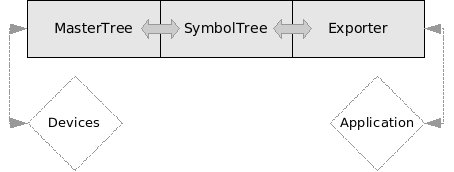
\includegraphics[scale=1]{cDCPU.png}
    \caption{Parts of the core.}
\end{figure}

The first called \textit{MasterTree}. This provide the access to the devices. The 
second part called \textit{SymbolTree} holds all values in a filesystem like 
hierachie. The last part, the \textit{Exporters}, serves the symboltree to other
applications like a visualisation. This concept is very common for this kind of 
problems. 

\subsubsection{The MasterTree}
To access the devices a master-slave based communication is often used. This are 
for example the common BUSes and also TCP/IP like networks. All these protocols
have one basic concept; they are seperable into layers. Each layer encapsulate 
an element of the communication.  For TCP/IP this is the famouse OSI reference 
model. So it is usefull to implement each layer of the communication channel
into separate modules to have the facility to reuse some of the modules. By
this you only need to implement these layers of the communication, that aren't
implemented yet to access a new device. For example if you want to access
a unsupported device that uses an allready implemented BUS you'll need only
to write a module that implements the command messages for this device.

A common way to seperate the communication is to differ between the used
interface, transport-protocol, and command-messages. The interface provides
the access to the BUS wardware, for example the serial-interface. The 
transport-protocol or BUS protocol uses the interface and generate valid 
messages that reaches the device. The module that generates the 
command-messages uses the transport-protocol to send the messages to the
device and to wait for an answer.  

\begin{figure}[ht]
    \centering
    \label{fig:cMasterTree}
    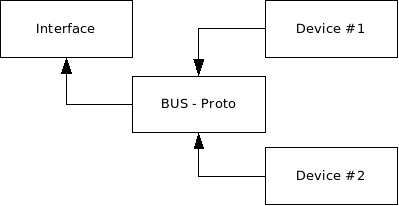
\includegraphics[scale=1]{cMasterTree.png}
    \caption{Scheme of MasterTree concept with shared interface and BUS modules.}
\end{figure}

An common cenario would be: You want to get a value from a device. So
you read from the module-object that implements the command messages.
This module will send a command-message over the BUS (protocol and interface)
to the device. Then the module will waits for an answer of the device
by reading from the BUS (over protocol and interface module). The
answer will be dispatched and you'll get the value.

If one module read from or writes to an other module the modules
will be locked and no other module can access these modules. By this way 
BUS collisions are avoided. And on the other hand if you want to access
two devices that are connected to the same BUS, you'll setup a 
MasterTree where the device-modules \#1 and \#2 share the modules for the 
interface and BUS. Now you see why the MasterTree is called a tree (forest 
would be better). The root of each tree is the interface and the leafes are 
the devices.

To get the all module work together a clear API between the modules have
to be defined, so that you don't have to adjust the modules to work together
with other/new modules. 

\subsubsection{The SymbolTree}
Once the access to the devices is seted up, you need to care about what values 
should be served. Each device will be able to provide a lot of different values
and a user or application don't know how to get a specific value. So you'll 
need a abstraction of the set of values. On the other hand, if you want to 
serve a lot of values you want to group the values by there sense and not by the
devices they are come from. So the idea of a \textit{filesystem} raises that holds 
the values in \textit{symbols} grouped in \textit{folders}, independent of the 
device the value was read from. At this point it will be usefull to control
who have access to a specific value (symbol). 

A symbol is usualy directly connected to a device-module. That means, if you 
want to get the value of the symbol, the symbol asks the device-module to read
the value from the device. But it is also possible to connect a symbol to a
module that implements a BUS protocol. By this you'll be able to tunnel the 
BUS to an other application of the internet. If you read out of such a symbol
you'll read directly from BUS and if you write into the symbol you'll write 
into the BUS. But be carefull with exporting the BUS to other networks, you
can't control what messages are sent over the BUS!

\subsubsection{Exporter}
The last part of the core exports the symboltree, or maybe a part of it, to
other applications. So the PPLT system is able to support a wide range of 
applications, independent of the protocol or interface the application
will use. Also the exporter are implemented as modules. But in this case
the comunication with the exporters are not seperated into seperate modules.
Each exporter is run into its own thread. So it is possible to handle
different applications with several instances at the same time. 


\section{Class description}
\begin{classdesc}{Core}{\optional{ModulePath, \optional{UserDBFile, \optional{LogLevel, \optional{LogFile, \optional{SysLog}}}}}}
This is the all-in-one class of the \module{pyDCPU}. All work like loding 
modules will be done by calling methods of this class. 

Creates a new core-instance. The optional argument \var{ModulePath} specifies
the basepath to the core-modules. If missed, the default path 
\texttt{sys.exec\_path+"/PPLT"} will be used. 

The argument \var{UserDBFile} specifies the filename of the used database to 
be loeded. If missed the default file 
(\texttt{sys.exec\_path+"/PPLT/UserDB.xml"}) will be used.


The argument \var{LogLevel} specifiy the loglevel and so the verbosity of the 
core. This shloud be one of (\code{'off'}, \code{'fatal'}, \code{'error'}, 
\code{'info'} or \code{'debug'}). Note that \code{'off'} switches the logging
off and \code{'debug'} will produce a lot of messages. 

In normal case all logging massages were printed on the screen (send to 
stderr) but with the arguments \var{LogFile} and \var{SysLog} you can 
manipulates this behavor. If the argument \var{LogFile} is given, this file 
will be used to log all messages to. Note, that if \var{LogFile} specified no 
messages are shown on stderr. If \var{SysLog} is \code{True} all log messages 
will be send to the local syslog-daemon. Note this argument overrides the 
setting of \var{LogFile} and also no messages were send to stderr.
\end{classdesc}

\section{Methods of \class{Core}}
\label{core-objects}
In the following section I will describe all methods of the \class{Core} 
class. 


\subsection{Mastertree methods}
\begin{methoddesc}[Core]{MasterTreeAdd}{ParentID, ModName, Address, Parameter}
This method loads an instance of a coremodule and adds it to the mastertree. 
The method returns the ID of the loaded mdoule. This ID is unique but if you 
load the same module with the same parameters, address and at the same parent, 
the ID of the allready loaded module will be returned. If an error accoures, 
the method will return \code{None}.

The argument \var{ParentID} specifies the parent-module (ID), the new loaded 
module will be attached to. If you set \var{ParentID} to \code{None} the 
module will be loaded as a root\footnote{A root-module has no parent module.}. 

The argument \var{ModName} specifies the full qualified name of the module. 
All modules are orgenized in classes and subclasses. A full qualified name 
would be a modulname with all classes and subclasses divided by single dots. 
For example: \code{Master.Interface.UniSerial} or \code{Master.Device.S7-200}.

The argument \var{Address} specifies the address used to connect the parent 
module. If there is no parent, meaning \var{ParentID} is \code{None}, or there
is no need to addressing the parentmodule, the argument \var{Address} should 
be \code{None}.

The argument \var{Parameter} specifies the parameter used to load (and setup) 
the module. This argument shlould be a dict.  The keywords are the parameters 
names (all strings) and the vlaues are the values of the singe parameter. \\ 
\note{All parameter values are strings!} If the module needs no parameters, 
please set \var{Parameter} to \code{None} or to an empty dict \code{\{\}}.
\end{methoddesc}


\begin{methoddesc}[Core]{MasterTreeDel}{ObjectID}
This method removes an (module-)object from the mastertree and destroy it. 
\note{The object mast have no chlidren, meaning no other objects  
are connected to this object.}

The argument \var{ObjectID} specifies the object you want to remove. This 
object ID is the ID you got by the \function{MasterTreeAdd()} method-call.

The method will return \code{True} if the object could be removed and destroyed 
and \code{False} otherwise.
\end{methoddesc}


\begin{methoddesc}[Core]{MasterTreeList}{ParentID}
This mehtod will list the IDs of all childen of the given moduleinstance. The argument \var{ParentID} specifies the 
ID of the moduleinstance, that children will be listed. 
\end{methoddesc}


\subsection{Symboltree methods}
\begin{methoddesc}[Core]{SymbolTreeCheckPath}{Path}
This method checks if the given \var{Path} exists. This method retuns  \code{True} if the given path is a folder or symbol
and \code{False} otherwise.
\end{methoddesc}


\begin{methoddesc}[Core]{SymbolTreeCreateFolder}{Path}
This method creates a folder. 

The argument \var{Path} specifies the full path to the folder, that will be creted. \note{The path should have the 
standrd Linux format like: \code{'/path/to/new\_folder'}.}

This method will return \code{Ture} if the folder was sucsessfully created and 
\code{False} otherwise.
\end{methoddesc}


\begin{methoddesc}[Core]{SymbolTreeCreateSymbol}{Path, ObjectID, \optional{Address}, \optional{Timeout}}
This method will creat a new symbol in the symboltree and connect it to the 
given Object.

The argument \var{Path} specifies the full path to the new symbol. This path 
should be in the standard Linux format like \code{'/path/to/new\_symbol'}.

The argument \var{ObjectID} specifies the object, the symbol will be connected
to. This is the ID you've got bach from a \function{MasterTreeAdd} call. You can 
connect a symbol to any object, but you'll not get allways usefull values back 
from this object. You can also connect the symbol to an object, that doesn't provide
any values, for example to a object of the \code{UniSerial} module to tunnel the
serial interface to an external application by the symboltree.

The optional argument \var{Address} specifies the address to be used to connect
to the object. To find out what addresses are provided by a specific module,
please look at the \textit{Core Modules Reference}. Of the address is obmitted,
no address will be used to connect to the object. In the most cases this means
to connect to the data chanel of the module. 

The optional argument \var{Timeout} specifies the cacheing time for the symbol in
seconds. The deault value is 0.5s.
For this time the last read value is returned instead of reread the value each 
time. By this it is possible to reduce the trafic on BUS if may clients access 
the symbols.
\end{methoddesc}


\begin{methoddesc}[Core]{SymbolTreeDeleteFolder}{Path}
This method will remove the given folder. This folder should be empty before removing it.

The argument \var{Path} specifies the path of the folder that will be removed. 

This method returns \code{True} on success and \code{False} on error.
\end{methoddesc}


\begin{methoddesc}[Core]{SymbolTreeDeleteSymbol}{Path}
This method will remove a symbol from the symboltree. 

The argument \var{Path} specifies the full path to the symbol, that will be removed.
This path should be in the standard Linux format like: \code{'/path/to/symbol'}.

This method will return \code{True} on success and \code{False} otherwise.
\end{methoddesc}


\begin{methoddesc}[Core]{SymbolTreeListFolder}{Path}
This method list all folders in the folder pointed by \var{Path}.

The argument \var{Path} specifies the full path to the folder, that subfolders
will be listed. 
\note{If you want to list all folders at the 
root-folder, you shloud use \code{'/'} as path.}

The method returns a list of strings or \code{None} if the path doesn't exists. The method will
return an empty list if the folder has no subfolders.
\end{methoddesc}


\begin{methoddesc}[Core]{SymbolTreeListSymbols}{Path}
This method will list all symbols in the folder pointed by \var{Path}.

The argument \var{Path} specifies the full path to the folder, that symbols
will be listed. 

\note{If you want to list all symbols at the 
root-folder, you should set \var{Path} to \code{'/'}.}

The method will return a list of strings or \code{None} if there are no 
symbols in the folder.
\end{methoddesc}


\begin{methoddesc}[Core]{SymbolTreeGetAccess}{Path}
This method will return the owner, group and accessrights of the given folder or symbol.

The argument \var{Path} specifies the path of the folder or symbol.
\end{methoddesc}


\begin{methoddesc}[Core]{SymbolTreeSetAccess}{Path, Owner, Group, Modus}
This method will set the owner, group and accessrights of the given symbol or folder.

The argument \var{Path} specifies the full path of the symbol or folder.

The argument \var{Owner} specifies the orwer of the symbol or folder, the 
argument \var{Group} specifies the group the symbol/folder will belong to.
At least the argument \var{Modus} spceifies the accessrights of the
symbol/folder.

This method will return \code{True} on success and \code{False} otherwise.
\end{methoddesc}


\begin{methoddesc}[Core]{SymbolTreeGetValue}{Path}
This method will return the value of the symbol pointed by \var{Path}.

The argument \var{Path} specifies the full path to the symbol. 

The method will return the value(s) of the symbol or \code{None} on error.
\end{methoddesc}


\begin{methoddesc}[Core]{SymbolTreeSetValue}{Path, Value}
This method will set the value of the symbol pointed by \var{Path} to \var{Value}.

The argument \var{Path} specifies the full path to the symbol, that value will be setted.

The argument \var{Value} specifies the value(s) the symbol will be setted to.

The method will return \code{True} on success or \code{False} else.
\end{methoddesc}


\subsection{Exporter methods}
\begin{methoddesc}[Core]{ExporterAdd}{ExportModule, Parameters, DefaultUser, \optional{Root='/'}}
This method will load and setup a exporter module. A exporter is something like
you may call a server.To sucessfully setup the module, some module specific 
parameters are needed. Also you can set a default user which rights will be 
used, if the exporter doesn't support any kind of authentication. Optional you can set 
a server-root. The server root should be a folder in the symbol tree. If a exporter 
is loaded with the \var{Root} option, only the symbols under the server-root 
and the subfolders of this root are exported by the server.

The argument \var{ExportModule} specifies the full qualified name of the 
exporter-module. A full qualified name kontains all classes and subclasses of 
the exporter. For example: \code{'Export.JVisu'}. 

The argument Parameters specifies the parameters, the export-module needs to be
successfully seted up. The parameters are given as a dict. The keys of the dict
are the names of the parameters and the values are the values of the 
parameters. If the export-module needs no parameters, please set 
\var{Parameters} to \code{None} or to an empty dict.

The argument \var{DefualtUser} specifies the name of the user, the server will 
get his rights from. This can be used to controll the rights of a exporter,
that doesn't know any authentication.

The optional argument \var{Root} specifies the server-root for this exporter. 
If you miss this argument or set it to \code{'/'}, the whole symboltree
will be exported by this server. Otherwise only the symbols and subfolders of
the given folder were be exported.

The method returns the ID of the exporter instance on success or \code{None}
on error.
\end{methoddesc}


\begin{methoddesc}[Core]{ExporterList}{}
This method lists the IDs of all loaded exports (servers). The method returns
a list of strings containing the IDs you got by the \function{ExporterAdd()}
methodcall. 
\end{methoddesc}


\begin{methoddesc}[Core]{ExporterDel}{ObjectID}
This method will stop and remove the exporter pointed by the given ID. 

The argument \var{ObjectID} specifies the exporter, that should be removed.
This is the ID you got by the \function{ExporterAdd} methodcall.

The method return \code{True} on success or \code{False} on error.
\end{methoddesc}

    \newcommand{\CoreModDesc}[1]{\newpage\subsection{#1}\index{Core Modules!#1}}
\newcommand{\CoreMod}[1]{\code{#1}}

\chapter{Core-modules Reference}
In this chapter I will describe all core (\module{pyDCPU}) modules.
A core module implements a new feature (protocol,device,...) to the
PPLT system. This is the atomic element of the PPLT devices and servers.

A core module is always a small python script with a specific interface 
zipped into an archive. This archive have to consists of at least two
files. One named \texttt{meta.xml} containing the meta-info of the
core-module. The second file have to be named \texttt{\_\_init\_\_.py}.
This file should include or contain the python source-code of the core
module.

In the following sections I will describe all core modules available until
now. Or all that I know of.



\section{Master modules}
Master modules are modules that are used in the PPLT devices. So this
modules implement the features to access a device, like the interface,
bus protocol, device commands, ...



%\CoreModDesc{Master.Interface.SendMail}
%This module implements the sending of e-mails via a
%specified SMTP host. \note{You have to have the permission 
%to send a e-mail of this host.} 



\CoreModDesc{Master.Interface.Socket}
This modules implements the basic TCP socket support for the PPLT system. 
With this module you can connect to other hosts over any tcp/ip based network
(Internet). This is used in the PPLT device \textit{PLC.FP-WEB} to connect to 
the tunneled ToolPort of a Panasoinc PLC. This module is able to hanle 
multible connections, so you don't need to load a 
\CoreMod{Master.Interface.Socket}-module for each connection you want.

\subsubsection{Parameters}
This module needs only one parameter:
\begin{tableiii}{l|p{10cm}|l}{textrm}{Parameter}{Description}{Default value}
\lineiii{TimeOut}
        {This parameter specifies the read-timeout for the socket 
         connection(s) in seconds. This should be a string with a floating 
         point number in it like '0.5' for a timeout of an half second.}
        {'0.0'}
\end{tableiii}

\subsubsection{Addresses}
This module need a address, thats specifies the host and port of the TCP 
connection. So if you connect to this module with an address "10.1.1.1:100"
a connection to the host "10.1.1.1" at the port 100 will be opend. See 
example for more details. \notice{If the connection to the host fails
the first time, it will be retryed each time you read/write from/to the 
module until the connection can be etablished.} 

\subsubsection{Example}
\begin{figure}[ht]
    \label{fig:coremod02}
    \centering
    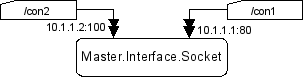
\includegraphics[scale=1]{coremod02.png}
    \caption{This figure shows the module-map of the socket-example.}
\end{figure}    
This example opens two connection to different hosts and ports:
\lstinputlisting{coremod02.py}



%
% Serial interface module:
%
\CoreModDesc{Master.Interface.UniSerial}
The \CoreMod{Master.Interface.UniSerial} core module implements the serial
interface for the PPLT system. This module needs the Python library 
\code{pySerial}. You can get this library from the URL 
\url{http://serial.sourceforge.net}. 

The settings of this module can be changed at runtime by symbols connected to
the addresses \emph{speed}, \emph{parity} \emph{timeout}.

\subsubsection{Parameters}
This module 4 parameters to setup. 
\begin{tableiii}{l|p{10cm}|l}{textrm}{Parameter}{Description}{Default value}
\lineiii{Port}
        {This is the number of the serial interface, the moudle should use. 0 
         means \code{ttyS0} or \code{COM1}, 1 means \code{ttyS1} etc. This
         parameter is not optional!}
        {---}
\lineiii{Speed}        
        {This is the speed in Baud the serial interface will be set to. This
         parameter is not optional!} 
        {---}
\lineiii{Parity}
        {This parameter specifies the parity check (settings) of the serial 
         inteface. 'Odd', 'Even', 'None' are valid values. This parameter
         is optional.}
        {'None'}
\lineiii{TimeOut}
        {This parameter sets the timeout for reading from the serial 
         interface in seconds. All floatingpoint numbers are valid an
         \code{None} means blocking-read.}
        {\code{None}}
\end{tableiii}
\notice{Some parameters can be reset at runtime by symbols connected to this 
module at special addresses. See next paragraph for details.}

\subsubsection{Addresses}
\begin{tableiii}{l|l|p{10cm}}{testrm}{Address}{Type}{Description}
\lineiii{---}
        {\code{TStream}}
        {This is the \emph{data-channel} to the serial-interface. Meaning 
         reading from this will read from the serial interface and writeing
         into a connection to this will write into the serial-interface.}
\lineiii{speed}
        {\code{TInteger}}
        {By this connector you'll be able to change the settings of the serial
         interface at runtime. Write an integer to a connection to this address
         will (try) to reset the baudrate to the value. See example for details.}
\lineiii{parity}
        {\code{TString}}
        {Writing strings like 'even', 'odd' or 'none' into this connector, will
         reset the setting of the serial interface. Reading from the connector
         will infrom you about the current setting.}
\lineiii{timeout}
        {\code{TFloat}}
        {Writing to this connector will reset the timeout for reading from 
         the serial interface.}
\end{tableiii}

\subsubsection{Example}
\begin{figure}[ht]
    \label{fig:coremod01}
    \centering
    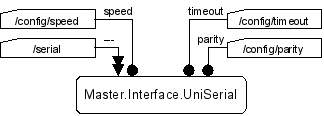
\includegraphics{coremod01.png}
    \caption{This figure shows the module-map of the UniSerial-example.}
\end{figure}    
This example shows how to setup the \CoreMod{UniSerial} and how to change the 
settings at runtime:
\lstinputlisting{coremod01.py}








%\CoreModDesc{Master.Interface.WGet}




%
% Transport layer of the Mewtocol:
%
\CoreModDesc{Master.Transport.MEWCOM-TL}
This module implements the transport-layer of the MEWTOCOL. The MEWTOCOL 
normally doesn't distinguish between the tansport and command layer. So
this module is only usfull in combination with the \CoreMod{MEWCOM-CL}
core-module that implements the command messages of the MEWTOCOL.

\subsubsection{Parameters}
This module needs only one parameter that specifies if a cecksum should
be calculated and adde to the MEWTOCOL message. By defualt this parameter
is set to \code{"True"}

\begin{tableiii}{l|p{10cm}|l}{textrm}{Parameter}{Description}{Default}
\lineiii{BCC}
        {This parameter specifies if a bcc (checksum) should be claculated
         for each packet send. This parameter doesn't contol the if the
         checksum of a recived packet will be checked. This will allways be 
         done (if the packet contains a checksum)\footnote{The MEWTOCOL 
         protocol allows that a packet doesn't contain a checksum. In this 
         case the checksum 'XX' will be set to indicate that the checksum
         should not be checked.}.  
        }{'True'}
\end{tableiii}       

\subsubsection{Addresses}
Each module or symbol have to set a address for the connection to this 
module. This address specifies the address of the destination the 
MEWTOCOL messages are send to. 
\begin{tableiii}{l|l|p{10cm}}{textrm}{Address}{Type}{Description}
\lineiii{0..255}
        {\code{TSequence}}
        {This address specifies the destination of the messages send.}
\end{tableiii}

\subsubsection{Example}
Because of this module is not usefull alone, please look at the example for 
the \CoreMod{MEWCOM-CL} core module.



%
% PPI module:
%
\CoreModDesc{Master.Transport.PPI}
This Core-Module implements the PPI protocol. It can be used to access the Siemens
SIMATIC S7 series PLCs. In this state of developing this module can't assable an
dispatch fragmentated packages. But in the most cases this is not needed. 

\subsubsection{Parameters}
This module needs only one parameter:
\begin{tableiii}{l|p{10cm}|l}{textrm}{Parameter}{Description}{Default}
\lineiii{Address}
        {This parameter specifies the PPI address of the PC. This is in the 
         most cases 0. But you have to set a value for this parameter!}
        {}
\end{tableiii}

\subsubsection{Addresses}
If you connect other modules or symbols to this module you'll need to specify
an address. This address is a number between 0 and 255. 
\begin{tableiii}{l|l|p{10cm}}{textrm}{Address}{Type}{Description}
\lineiii{0-255}{\code{Sequence}}
        {This address specifies the address of the device in the PPI BUS. 
         Writeing into the connection will cause a packet send to the device
         addressed by this address. Also reading from the connection will only
         return the content addressd to the setted Parameter \var{Address} and
         from the device addressd by this address.}
\end{tableiii}

\subsubsection{Example}
\begin{figure}[ht]
    \label{fig:coremod07}
    \centering
    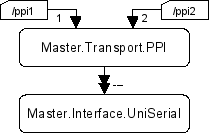
\includegraphics{coremod07.png}
    \caption{This figure shows the module-map of the PPI-example.}
\end{figure}    
This example shows how to tunnel the PPI bus by the symbol tree. For an more
usefull example please look the the Example for the \CoreMod{S7} core-module.
\lstinputlisting{coremod07.py}



%
% ReadLine module.
%
\CoreModDesc{Master.Transport.ReadLine}
This module can be used if you want to do some line-orientated communication.

This is often used for simple protocols for the serial interface. For example
the AT commands for modems but also the Mewtocol by Panasonic (FP0 and FP1) 
uses a line-orientated protocol to send or recive commands to/from the PLC.  

So this module have to be used as a child of a module that provides
\code{TStream} or \code{TSequence} connections.

\subsubsection{Parameters}
This module needs a parameter to specify the \emph{line-end} character(s).
\begin{tableiii}{l|p{10cm}|l}{textrm}{Paramter}{Description}{Default}
\lineiii{LineEnd}
        {A hex-encoded string that the module will use as a sign for the 
         line-end. And also all data send over this module will be extended
         with this string.}
        {0A0D} 
\end{tableiii}

\subsubsection{Addresses}
This module knows only one address: no address.
\begin{tableiii}{l|l|p{10cm}}{textrm}{Address}{Type}{Description}
\lineiii{---}
        {\code{TSequence}}
        {All data written into this connector will be extended by the set 
         line-end. And also if you read from this connector it will block 
         until the set line-end character(s) appear in the data-stream.
         \textbf{Note:} The whole line will be then returned!}
\end{tableiii}

\subsubsection{Example}
\begin{figure}[ht]
    \label{fig:coremod10}
    \centering
    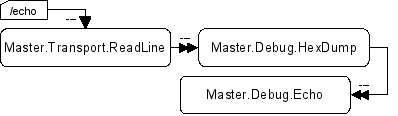
\includegraphics{coremod10.png}
    \caption{This figure shows the module-map of the ReadLine-example.}
\end{figure}    
This example shows on the one hand the usage of the \CoreMod{ReadLine} module.
On the other hand it is a quite good test for the \CoreMod{Echo} module. 
This example write a string into \CoreMod{ReadLine} that extends the string 
with the line-end. Then it will send this message to the \CoreMod{Echo} module.
Then it trys to read from \CoreMod{ReadLine} that trys to read a complete 
line from his parent (\CoreMod{Echo}) strips the line-end characters and
return the string. If all goes well the same string will be returned. To see
what's going on a \CoreMod{HexDump} module will be plugged between the 
\CoreMod{Echo} and \CoreMod{ReadLine} modules.
\lstinputlisting{coremod10.py}



%
% Agilent 5462x series oscilloscopes 
%
\CoreModDesc{Master.Device.5462X}
This module implements the command messages to access an Agilent 
oscilloscopes. This module only supports the message format used 
by the serial interface of the oscilloscope. So you need to connect
this module (indirect) to the \CoreMod{Master.Interface.UniSerial}
core-module.

\subsubsection{Parameters}
This module need two parameters to be set up. These parameters specify the
primary and secondary signal source. If you only want to use the primary
source you should set the secondary to the same source like the primary.
\begin{tableiii}{l|p{10}|l}{textrm}{Parameter}{Description}{Default}
\lineiii{PSource}
        {This specifies the primary source. This can be one of A0 (analog \#1),
         A1 (analog \#2), M (math) or F (form).}{---}
\lineiii{SSource}
        {This specifies the secondaray source. Look at \var{PSource} for more
         details}{---}
\end{tableiii}         
\bf{To be continued}\bf{To be continued}

%
% Panasonic A200 Imagechecker
%
%\CoreModDesc{Master.Device.A200}



%
% GSM compatible mobile-phone.
%
\CoreModDesc{Master.Device.GSM}



%
% Command-messages for the Panasonic FP0 and FP1
%
\CoreModDesc{Master.Device.MEWCOM-CL}
This core-module implements the command messages of the MEWTOCOL. This 
protocol is used to access the Panasonic FP0 FP2 PLCs. So you can access
the markers of these PLCs using the \CoreMod{Master.Transport.MEWCOM-TL},
\CoreMod{Master.Device.MEWCOM-CL} core-modules and a interface module like 
\CoreMod{Master.Interface.UniSerial} or \CoreMod{Master.Interface.Socket}.

\subsubsection{Parameters}
This module needs no parameters to be set up.

\subsubsection{Addresses}
You have to set a address to connect a symbol to this module! With this 
address you specify the marker you want to get/set. Additional there is a
address called \code{"STATUS"} that controls the state of the PLC 
(\emph{run}/\emph{stop}).
\begin{tableiii}{l|p{2cm}|p{10cm}}{textrm}{Address}{Type}{Description}
\lineiii{STATUS}
        {\code{TBool}}
        {By this address you can control the state of the PLC. If it is 
         \code{True} then the PLC is in the \emph{Run} mode. You can also
         get the state of the PLC by reading this value.}
\lineiii{\emph{Marker}}
        {\code{TBool} or
         \code{TInteger}}
        {By setting a marker-address as the address for the connection to this 
         module, you are able to access (read/write) this marker. So the type 
         of the connection you'll get depends on the marker-address you set.} 
\end{tableiii}

\subsubsection{Example}
\begin{figure}[ht]
    \label{fig:coremod11}
    \centering
    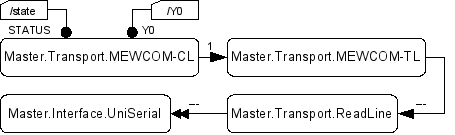
\includegraphics{coremod11.png}
    \caption{This figure shows the module-map of the MEWCOM-CL example.}
\end{figure}    
This example shows how to access a FPx using the \emph{ToolPort} (serial interface).

\lstinputlisting{coremod11.py}



%
%
%
\CoreModDesc{Master.Device.S7}
This module implements the command-messages of the Siemens SIMATIC S7(-200). 
With this module and the \CoreMod{Master.Transport.PPI} and 
\CoreMod{Master.Interface.UniSerial} it is possible to access the S7 over the 
PPI bus. To do this you must configure the serial interface in a special way. 
Look at the example to find out how. This module can generate messages that 
cause the S7 to send the value of the requested marker. To specify the marker 
you want to get you have to connect a symbol with this module with the name of
the marker as address. It could be possible that not all availabe marker can be
read. If you know some of them please let me know.

\subsubsection{Parameters}
This module needs no parameters to be set up.

\subsubsection{Addresses}
The address you have to specify to connect a symbol to this module should be 
the name of the marker you want to get/set.
\begin{tableiii}{l|p{2cm}|p{10cm}}{textrm}{Address}{Type}{Description}
\lineiii{\emph{Marker}}
        {\code{TBool}, \code{TInteger}}
        {With the address you specify the marker you'll access. So the type 
         of the values you'll get depends on the marker you'll set. So if you 
         access an boolean marker you'll get values typed \code{TBool} if you
         access byte,word and double word Markers you'll get values types
         \code{TInteger}.}
\end{tableiii}

\subsubsection{Example}
\begin{figure}[ht]
    \label{fig:coremod08}
    \centering
    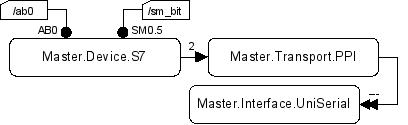
\includegraphics{coremod08.png}
    \caption{This figure shows the module-map of the S7-example.}
\end{figure}    
In this example I'll access (read/write) the markers SM0.5 (special marker 0 bit 5) and AB0
(output byte 0).

\lstinputlisting{coremod08.py}



%
% ECHO module
%
\CoreModDesc{Master.Debug.Echo}
This module echoes all data writte to it at reading from it. It can be used to
debug other modules. This is a so called \emph{root}-module. It can't be 
loaded as a child of an other module!

\subsubsection{Parameters}
This module needs no parameters!

\subsubsection{Addresses}
This module has only one addresses: no address.
\begin{tableiii}{l|l|p{10cm}}{textrm}{Address}{Type}{Description}
\lineiii{---}
        {\code{TStream}}
        {If you write into a symbol connected to this module, the data will be
         buffered and the next time you read from it the buffer (or a part of 
         it) will be returned.}
\end{tableiii}

\subsubsection{Example}
\begin{figure}[ht]
    \label{coremod06}
    \centering
    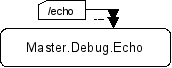
\includegraphics{coremod06.png}
    \caption{This figure shows the module-map of the Echo-example.}
\end{figure}    
This is a simple echo-example... ... the classic.

\lstinputlisting{coremod06.py}



%
% HexDump Module 
%
\CoreModDesc{Master.Debug.HexDump}
This module is a simple trafic dumper. It dumps all data going throught it
into the logging-system with loglevel \emph{debug}. So you can read it from
your logfile or \code{stderr}. Simply plug this module between two modules
to record all trafic.

\subsubsection{Parameters}
This module needs no parameters!

\subsubsection{Addresses}
This module has only one address: no address! 
\begin{tableiii}{l|p{2cm}|p{10cm}}{textrm}{Address}{Type}{Description}
\lineiii{---}
        {\code{TStream} or \code{TSequence}}
        {All data written to this module will be written to the parent and 
         read vica versa. So the type of the connection will depend on the
         type of the parent-connection.}
\end{tableiii}

\subsubsection{Example}
\begin{figure}[ht]
    \label{fig:coremod05.py}
    \centering
    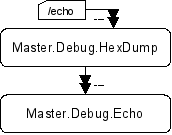
\includegraphics{coremod05.png}
    \caption{This figure shows the module-map of the HexDump-example.}
\end{figure}    
This module uses the echo module to show how the trafic in read and write 
direction will be dumped:
\lstinputlisting{coremod05.py}



%
% Null module (the black hole)
%
\CoreModDesc{Master.Debug.Null}
This is a very simple module, that works like the /dev/null device file on 
Linux. If you read from this module, you'll get a string with zero-bits and
if you write into this module nothing will happens. This module swallow all
you write into it.

\subsubsection{Parameters}
This module needs no parameters to be set up.

\subsubsection{Addresses}
This module has only one valid address: no address.
\begin{tableiii}{l|l|p{10cm}}{textrm}{Address}{Type}{Description}
\lineiii{---}
        {\code{TStream}}
        {This will be the connection to the \CoreMod{Null} module. Id you
         write into this connection the module will swallow all data and
         nothing will happen. If you read from this module you'll get a 
         stream of zero-bits.}
\end{tableiii}

\subsubsection{Example}
\begin{figure}[ht]
    \label{fig:coremod09}
    \centering
    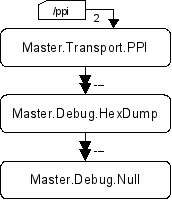
\includegraphics{coremod09.png}
    \caption{This figure shows the module-map of the Null-Example.}
\end{figure}    
This example shows a configuration to debug a non \emph{root} module. In this 
case it is the \CoreMod{Master.Transport.PPI} core-module. To get some 
information about the packages the PPI module sends the core-module 
\CoreMod{Master.Debug.HexDump} is used.  \notice{This example raises an 
exception, because the PPI module expect a correct answer from the 
\emph{virtual} device (in this case the core-module 
\CoreMod{Master.Debug.Null}).
\lstinputlisting{coremod09.py}



%
% Random-generator module
%
\CoreModDesc{Master.Debug.Random}
This module implements a random-generator, that can generate data for every 
symbol-type supported by the \module{pyDCPU}. So this module can be used to 
test almost all facilities of the system. 

\subsubsection{Parameters}
This module needs no parameters. 

\subsubsection{Addresses}
\begin{tableiii}{l|l|p{10cm}}{testrm}{Address}{Type}{Description}
\lineiii{Bool}
        {\code{TBool}}
        {Provide a random boolean value.}
\lineiii{Integer}
        {\code{TInteger}}
        {Provide a random integer value between 0 and 100.}
\lineiii{Float}
        {\code{TFloat}}
        {Provide a random floating point number between 0 and 1.}
\lineiii{String}
        {\code{TString}}
        {Provide a random string of a random length between 1 and 79 containg 
         printable characters.}
\lineiii{ArrayBool}
        {\code{TArrayOfBool}}
        {The name tells everything. The length of the array is randomly 
         between 1 and 3.}
\lineiii{ArrayInteger}
        {\code{TArrayOfInteger}}
        {Array of integer of random length between 1 and 3.}
\lineiii{ArrayFloat}
        {\code{TArrayOfFloat}}
        {Array of floating point numbers with variable length between 1 and 
         3.}
\lineiii{ArrayString}
        {\code{TArrayOfString}}
        {Array of string with variable length (of array) between 1 and 3.}
\lineiii{Stream}
        {\code{TStream}}
        {Provides an random data string. The data are printable character.
         The number of bytes returned is less than equeal the number you 
         wanted to read. To read from a symbol connected to this address,
         please use the method \method{SymbolTreeRead().}}
\lineiii{Sequence}
        {\code{TSequence}}
        {A sequence of random data. The data contains only printable 
         characters and the length varies between 1 and 79.}
\end{tableiii}

\subsubsection{Example}
This is a simple example that uses all types:
\lstinputlisting{coremod03.py}



%
% Statistic module
%
\CoreModDesc{Master.Debug.Statistic}
This module collects statistical values of the data flowing through it. You 
can use this module to improve or debug your own modules or even to observe
the PPLT system. This module is quite easy to use: simply plug this between 
two other modules and you are able to observe the trafic between them.
\notice{You can only observe modules that provides a \code{TStream} or 
\code {TSequence} connection.}

\subsubsection{Parameters}
This module needs no parameters!

\subsubsection{Addresses}
There are several addresses provideing the statistical data. If you use no 
address to connect to this module a \code{TStream} or \code{TSequence} 
connection to the parent will be returned. This connection to the parent will
be used to collect the statistical data. 

\begin{tableiii}{l|p{2cm}|p{10cm}}{textrm}{Address}{Type}{Description}
\lineiii{---}
        {\code{TStream} or \code{TSequence}}
        {This is the data-tunnel to the parent of the 
         \CoreMod{Statistic}-module. The type of the connection depends on
         the type of the connection to the parent module. You see, it is only
         possible to connect the \CoreMod{Statistic}-module to a parent that
         provides a \code{TStream} or \code{TSequence} connection.}
\lineiii{read\_data}
        {\code{TInteger}}
        {Returns the number of bytes read from the parent.}
\lineiii{write\_data}
        {\code{TInteger}}
        {Returns the number of bytes written to the parent.}
\lineiii{read\_speed}
        {\code{TFloat}}
        {Returns the number of bytes per second read from parent since 
         module-loading. This value is the average of the whole time since
         module-loading.}
\lineiii{write\_speed}
        {\code{TFloat}}
        {Returns the number of bytes written to the parent since the module 
        was loaded. This value is the average of the whole time.}
\lineiii{error}
        {\code{TInteger}}
        {Returns the number of read/write-errors since the module was loaded.
         This must not be an indicatior for bugs in the parent modules because
         also timeouts will be recorded.}
\end{tableiii}

\subsubsection{Example}
In this example the serial interface will be exported by the symbol tree.
The \CoreMod{Statistic}-module records the trafic throught the serial 
interface.
\lstinputlisting{coremod04.py}



\newpage
\section{Export modules}
\CoreModDesc{Export.JVisu}
\CoreModDesc{Export.SimpleExport}
\CoreModDesc{Export.PPLTWeb}


    
    
    \newcommand{\PSFTag}[1]{\index{PSF Elements!#1}}



\chapter{PSF Reference --- \textbf{P}PLT \textbf{S}ession \textbf{F}ile}

This section describes the file-format of the PPLT session files. Such 
files contain the information about the state of the system. 
So the file contains information about the loaded devices and servers and
also the layout of the symbol-tree.

Files formatted in the PSF format can be created from a running PPLT system by 
a call of the method \method{SaveSession()} and can then be loaded by a 
\method{LoadSession()} method-call.

By this way you can easily implement a simple daemon or service, that reads 
such a PSF file and setup a whole PPLT system. Meaning loading all devices, 
creating all symbols and folders and at the end loading all servers.

All you need to know is a basic knowledge of XML formats, and a little idea of 
what PPLT is and what the system needs to save (or even needs to know to setup
the PPLT system). 

\section{Reference}
In the following section I'll list all keyword of the PSF format. These are only few
because the format stills easy. 

At first: The PSF format is an XML format!

\subsection{\keyword{PPLTSession}}
\PSFTag{PPLTSession}
The PPLTSession tags surround the PPLT session document. Containing all 
information about the devices, servers and symbol-tree. This tag must
(directly) contain the elements (tags) \keyword{Servers}, \keyword{Devices}
and \keyword{SymbolTree}. But each elements can only occur once.
This also defines the basic layout of the PPLT session document. Each document
should look like:
\begin{verbatim}
<?xml version="1.0"?>
<PPLTSession>
    <Servers>
        [...]
    </Servers>
    <Devices>
        [...]
    </Devices>
    <SymbolTree>
        [...]
    </SymbolTree>
</PPLTSession>
\end{verbatim}


\subsection{\keyword{Servers}}
\PSFTag{Servers}
The tag \keyword{Servers} contains the description of all loaded servers. This tag can only 
contain any occurrence of the tag \keyword{Server}. Each \keyword{Server}-tag describe a 
singe server to load. For more details see at the description of the \keyword{Server}-tag.

\begin{verbatim}
[...]
    <Servers>
        <Server [...]>
            [...]
        </Server>
        [...]
    </Servers>
[...]
\end{verbatim}


\subsection{\keyword{Server}}
\PSFTag{Server}
The tag \keyword{Server} describes a server to load. The tag can only contain any occurrence of the tag
\keyword{Parameter}. Each \keyword{Parameter} tag specifies a parameter needed to load the server.
Also the \keyword{Server} needs some attributes. The attribute \var{alias} specifies the alias the
server will get after it was loaded. The attribute \var{fqsn} specifies the full-qualified-server-name. 
This unique name specifies the server to be loaded. The Attribute \var{root} specifies the server root.
\note{The given server-root but exist else the loading of the server will fail.} The attribute 
\var{user} specifies the default user. The server will run with the rights of this user, if the 
server doesn't know any authentication. 

A simple example will can be:
\begin{verbatim}
[...]
    <Server alias="JVisu" fqsn="Visu.JVisuServer" root="/" user="admin">
        <Parameter name="Port">2200</Parameter>
        <Parameter name="Address">127.0.0.1</Parameter>
    </Server>
[...]
\end{verbatim}
This example will start a JVisu server with the rights of the user \code{admin} and
with the server root \code{'/'}. JVisu is a open source visualization written in Java.
You can get it from \url{http://jvisu.sourceforge.net}.

\subsection{\keyword{Parameter}}
\PSFTag{Parameter}
The \keyword{Parameter}-tag specifies a parameter, the system will use to setup
a \keyword{Server} or \keyword{Device}. The \keyword{Parameter}-tag can only 
contain CDATA, meaning it can only contain a string. The content will be 
interpreted as the value of the parameter. The \keyword{Parameter}-tag
knows also a attribute. The attribute \var{name} specifies the name
of the parameter. To find out what parameters are needed to setup
a specific server, please consult the Device and Server reference.


\subsection{\keyword{Devices}}
\PSFTag{Devices}
Like the \keyword{Servers}-tag this tag contains the description of
all devices needed to be loaded. So this tag can only contain any
occurrence of the tag \keyword{Device}. For example:
\begin{verbatim}
[...]
    <Devices>
        <Device [...]>
            [...]
        </Device>
        [...]
    </Devices>
[...]
\end{verbatim}


\subsection{\keyword{Device}}
\PSFTag{Device}
Like the \keyword{Server}-tag this tag describes one device to load. Also it can only contain 
any number of \keyword{Parameter} tags to specify the the parameters the device may need to be
loaded. It also has some attributes. The attribute \var{alias} specifies the alias the device 
gets when it's was successfully loaded. The attribute \var{fqdn} specifies the full qualified 
device name. This is the name of the device you want to load.

For example, a \keyword{Devices}-section can be:
\begin{verbatim}
[...]
    <Devices>
        <Device alias="rand" fqdn="Debug.RandomGenerator"/>
        <Device alias="S7" fqdn="PLC.S7-200">
            <Parameter name="PCAddr">0</Parameter>
            <Parameter name="Port">1</Parameter>
            <Parameter name="S7Addr">2</Parameter>
        </Device>
    </Devices>
[...]
\end{verbatim}
This example will load a random-generator as \code{'rand'}  and the support for the Siemens SIMATIC S7-200 
as \code{'S7'}.


\subsection{\keyword{SymbolTree}}
\PSFTag{SymbolTree}
The \keyword{SymbolTree}-section describes the content of the symbol-tree. So this tag can only contain
any occurrence of \keyword{Symbol} and \keyword{Folder} tags. This tag don't take any attributes.

\subsubsection{How the symbol-tree is depicted}
The symbol-tree works like a small filesystem, with folders, sub-folder and symbols. The root of this filesystem is the
symbol-tree itself. Now you need to know how to depict the hierarchy of the symbol-tree to an XML file.

I think the best way to describe is to give an example. The following symbol-tree hierarchy
\begin{verbatim}
/
/FOLDER1/
/FOLDER1/FOLDER2/
/FOLDER1/FOLDER2/Symbol1
/FOLDER1/FOLDER2/Symbol2
/FOLDER1/Symbol3
/FOLDER3/
/FOLDER3/Symbol4
/Symbol5
\end{verbatim}
will be depicted as something like:
\begin{verbatim}
<SymbolTree>
    <Folder name="FOLDER1">
        <Folder name="FOLDER2">
            <Symbol name="Symbol1"/>
            <Symbol name="Symbol2"/>
        </Folder>
        <Symbol name="Symbol3"/>
    </Folder>    
    <Folder name="FOLDER3">
        <Symbol name="Symbol4"/>
    </Folder>
    <Symbol name="Symbol5"/>
</SymbolTree>
\end{verbatim}
As you see; the \keyword{SymbolTree} can contain \keyword{Symbol}s and \keyword{Folder}s. And each \keyword{Folder} can
also contain \keyword{Symbol}s and \keyword{Folder}s. But only the \keyword{Symbol}s are empty, because they can't contain
anything. In this example I missed some additional attributes to avoid you to be confused. This attributes are described 
in detail in the following sections.

\subsection{\keyword{Symbol}}
\PSFTag{Symbol}
The \keyword{Symbol}-tag describes a symbol of the symbol-tree. Such a symbol is a kind of a variable that can hold values.
Each symbol is connected to a so called "symbol-slot"\footnote{A symbol-slot always belongs to a device, so if you want to know 
what slots are provided by a specific device, pleas look at the documentation of the device.}. So you need to specify the 
symbol-slot the symbol will be connected to by the attribute \var{slot}. The slot-name must be provided in the format 
\code{'DEVICE\_ALIAS::NAMESPACE::SLOT\_NAME'}. The \code{DEVICE\_ALIAS} specifies the device you want the symbol to be
connected to. It should be the string you give to the \keyword{Device}-attribute \var{alias}. The \code{NAMESPACE}s and
\code{SLOT\_NAME}s are provided by the devices. To find out what namespaces are available, look at the documentation of 
each device.

In this context you also need to define the type of the symbol by the attribute \var{type}. The type is defined by the
slot you use. So please take a look at the documentation of the specific device.

Now your symbol can get and (maybe) set values. But a major feature of the PPLT is, that you can control the
access to the symbol by setting rights to it. To do so, you need to set a \var{owner}, \var{group} and
\var{modus} to the symbol (and also to the folder). So a complete example for a symbol that is connected to
a random-generator loaded as \code{'rand'} could be:
\begin{verbatim}
[...]
    <SymbolTree>
        <Symbol name="r_bool" slot="rand::Generator::Bool" type="Bool" 
                owner="admin" group="Admin" modus="600"/>
        [...]
    </SymbolTree>
[...]
\end{verbatim}
You see the attribute \var{modus} contains a 3-digit integer. This integer is calculated like the Linux modus integer. Pleas look
at the \manpage{chmod}{} man-page to get more information. But sofar the number \code{600} says that only the owner has the right to 
read/write to the symbol and the group and any other has no rights.


\subsection{\keyword{Folder}}
\PSFTag{Folder}
The \keyword{Folder}-tag describes a folder in the symbol-tree. The name of the folder will be specified by the
attribute \var{name}. Like the symbols a folder also owned by a user and attached to a group. So you also need 
to set the \var{owner}, \var{group} and \var{modus} attributes. 

\newpage
\section{A complete Example}
In the following section I'll show you a complete example of a PSF. The file describes two devices, a random generator and
a Siemens SIMATIC S7-200. The symbol-tree contains two folders one, named 'Rand', will contain some symbols connected
to the random-generator and the other, named 'S7' will contains the symbols connected to the S7. And a web-server will be loaded, 
that exports the whole symbol-tree. 

\verbatiminput{PSF.xml}



    
    \documentclass{manual}

\title{PPLT References}
\author{Hannes Matuschek\\\texttt{<hmatuschek@gmx.net>}}
%\date{2005-10-12}
\release{0.9.0}
\setshortversion{0.9.0(beta)}
\makeindex


 \begin{document}
   
    \maketitle
    \begin{abstract}
    This document summarize the references of the PPLT system. Including Core-Library reference, reference
    of the PPLT abstraction layer, documenttypes and some other stuff.
    \end{abstract}

    \tableofcontents


    \chapter{PPLT Reference}
\section{\module{PPLT} ---
        \textbf{P}otsdamer \textbf{P}rozess \textbf{L}eit \textbf{T}echnik}

\declaremodule{}{PPLT}
\moduleauthor{Hannes Matuschek}{hmatuschek@gmx.net}
\modulesynopsis{The PPLT is a framework for master/slave based communication.}

The \module{PPLT} builds an abstraction layer over the core library 
(\module{pyDCPU}). With the PPLT you can easily handle abstract devices and 
server instead of handle with several core modules. Like the core-library the 
PPLT has only one class called \code{System}. After instancing this class, all
work can be done by calling the methods of this object.

\section{Class description}
\begin{classdesc}{System}{\optional{BasePath}, \optional{CoreLogLevel}, 
\optional{PPLTLogLevel}, \optional{LogFile}, \optional{Syslog}, 
\optional{Lang}, \optional{AltLang}}
This is the all-in-one class. If this class will be instanced the complete 
PPLT system will be loaded. Meaning searching plug-ins (modules), loading 
user-database, starting core-system, etc...

The argument \var{BasePath} specifies the path of all PPLT related stuff. This 
is by default \code{sys.exec\_prefix+'/PPLT'}. Under Windows this is the folder 
where you've installed Python under \UNIX this should be some thing like 
\code{/usr/local/PPLT}. If you miss this argument, the default path will be 
used.

The argument \var{CoreLogLevel} specifies the log-level for the core library. 
This should be one of \code{off}, \code{fatal}, \code{error}, \code{warning}, 
\code{info}, \code{debug}.  If you select \code{debug} a lot of (not always 
useful) messages will be logged and \code{off} switches the logging off. 
By default the logging level \code{info} will be used. If you miss this 
argument, the default value will be used.

The argument \var{PPLTLogLevel} specifies the log-level of the PPLT library. 
This should be one of \code{off}, \code{fatal}, \code{error}, \code{warning}, 
\code{info}, \code{debug}. If you select \code{debug} a lot of (not always 
useful) messages will be logged and \code{off} switches the logging off. 
By default the logging level \code{info} will be used. If you miss this 
argument, the default value will be used.

The argument \var{LogFile} specifies the file,  where the logging messages are
written to. If you missed this argument, there were no messages written to any
file, all messages were send to screen (\code{stderr}). 

The boolean argument \var{SysLog} specifies if the messages should be send to
the local \code{syslog}-daemon. 
\begin{notice}
This argument overwrites the optional argument \var{LogFile}. If \var{SysLog}
it \code{True} no messages were written into any file nor send to screen!
\end{notice}
By default this argument if \code{False}. If you missed this argument, the 
default will be used.

The argument \var{Lang} specifies the primary language the system will use for
module description. This option do not change the language of the logging 
messages (they are not translated). This option is not important for normal
usage of the PPLT. By default \code{'en'} will be used.

The argument \var{AltLang} specifies the alternative language to be used
for module description. This should be always \code{'en'}. \textbf{Do not 
change until you know what you do.} 

If the primary language can not be found, the alternative will be used. 
\end{classdesc}




\section{Methods of \class{System}}
In this section I will describe the methods of the \class{System}-class. I 
will not list all available methods, because there are more then 60 of it. Some
of them are only useful if you want to write a GUI application like the
\emph{PPLT Center}. But you can get a short help over all methods by calling
\code{pydoc PPLT.System}. 


\subsection{Device methods}
\begin{methoddesc}[System]{LoadDevice}{DeviceName, Alias, Parameters}
This is one of the most important methods. With this method you can load and
setup a device. This method loads the device \var{DeviceName} as \var{Alias}. 
The alias will be used later to specify this device, for example if you want
to connect a symbol to this device or unload the device.

The argument \var{DeviceName} specifies the full qualified device name. All
devices (and servers) are grouped by classes. A full qualified device name
consists always of all classes and the name divided by a single dot. For
example \code{'PLC.Panasonic-FPX'}.

The argument \var{Alias} specifies the alias the device will get after being
loaded. By this alias you will identify the device later.

The attribute \var{Parameters} specifies the parameters the device needs to be
set up successfully. This should be a dict with key-value pairs. The key 
is the parameter name and the value should be the parameter-value. For example:
\code{\{'Port':'0', 'Address':'123'\}}.
\begin{notice}
All parameter names and also \textbf{all} parameter values are strings!
\end{notice}

This method will return \code{Ture} on success an \code{False} on error.
\end{methoddesc}


\begin{methoddesc}[System]{UnLoadDevice}{Alias}
This method unload and destroy the given device. 

The argument \var{Alias} specifies the alias of the device you want to be
unloaded. This is the alias you've set at the \method{LoadDevice} 
method-call.

This method returns \code{True} on success and \code{False} on error.
\end{methoddesc}


\begin{methoddesc}[System]{GetFQDeviceName}{Alias}
This method returns the full qualified device name of the device loaded as
\var{Alias}.

The attribute \var{Alias} specifies the alias of the loaded device. This is
the alias you've set at the \method{LoadDevice} method-call.

This method returns a string containing the full qualified device name or non 
if the alias if not a device or not loaded.
\end{methoddesc}


\begin{methoddesc}[System]{GetDeviceParameters}{Alias}
This method will return the parameters the device was loaded with. This method
will return a dict on success or \code{None} on error.
\end{methoddesc}


\subsection{Server methods}
This section describes all methods to handle servers, like starting, stopping, ... 

\begin{methoddesc}[System]{LoadServer}{ServerName, Alias, DefaultUser, Parameters\optional{, Root}}
This method loads and setup a server. 

The argument \var{ServerName} specifies the full qualified server name. Full 
qualified means that all classes and the name are given, divided by a single 
dot (like: \code{Web.PPLTWebServer}).

The argument \var{Alias} specifies the alias the server will have after 
being loaded. By this alias you will identify the server later, for example 
to unload this server.

The argument \var{DefaultUser} specifies the the user, the server will run as. 
By this option you can assign rights to a server, that doesn't know any 
authentication. By default, a server should support a authentication but 
sometimes the used protocol doesn't (for example JVisu). For this kind of 
server this option is useful.

The argument \var{Parameters} specifies the parameters the server will be 
loaded with. This should be a dict with the parameter name as key (string)
and the parameter value as value (also a string!). If a server doesn't needs
any parameters, please set \var{Parameters} to \code{None} or to and empty 
dict (\code{\{\}}). 

The optional argument \var{Root} specifies the server-root of this server. 
By default (\var{Root}=\code{'/'}) the whole symbol-tree will be accessible
by this server. But if you want to export only a specific folder of the 
symbol-tree you can specify this folder with the \var{Root} argument. So
if \var{Root}=\code{'/test'} only the content of the folder \code{'/test'}
will be accessible by this server.

This method returns \code{True} on success and \code{False} else.
\end{methoddesc}


\begin{methoddesc}[System]{UnLoadServer}{Alias}
This method will stop and destroy a server loaded with \method{LoadServer}.

The attribute \var{Alias} specifies the server you want to stop. This is the 
alias you've defined on loading the server with \method{LoadServer}.

This method will return \code{True} on success and \code{False} else.
\end{methoddesc}


\begin{methoddesc}[System]{GetFQServerName}{Alias}
This method will return the full qualified server-name of the loaded server
by his alias. 

The argument \var{Alias} specifies the alias of the server. This is the alias
you have defined on loading by the \method{LoadServer} method.

This method returns a string on success or \code{None} on error.
\end{methoddesc}


\begin{methoddesc}[System]{GetServerParameters}{Alias}
This method will return the dict of parameters the server was loaded with. 
This is the parameter dict, you have defined on loading the server with 
\method{LoadServer}.

The argument \var{Alias} specifies the alias of the loaded server. This is
the alias you have defined on loading the server with \method{LoadServer}.

This method will return a dict or \code{None} on error. This method will
return an empty dict even if you've loaded the server with no parameters.
\end{methoddesc}


\begin{methoddesc}[System]{GetServerRoot}{Alias}
This method will return the server root of a loaded server. This is the 
server root you have defined on loading the server with \method{LoadServer}.

The server root is the base folder in the symbol-tree the server can access. 
Only folders and symbols laying under this folder are accessible by this 
server.

The argument \var{Alias} specifies the alias of the loaded server. This is the
alias you have defined on loading the server with \method{LoadServer}. 

This method will return a string on success or \code{None} on error.
\end{methoddesc}


\begin{methoddesc}[System]{GetServerDefaultUser}{Alias}
This method will return the default-user the server is running with. This is
the username you have defined on loading the server with \method{LoadServer}.

If specified, the server will run with the rights of the default user. This is
necessary, because there are some servers which don't know any authentication!

The argument \var{Alias} specifies the alias of the loaded server. This is the 
alias you have defined for this server on loading with \method{LoadServer} 
call.

This method will return a string on success or \code{None} on error.
\end{methoddesc}


\subsection{Symboltree methods}
In the following section I will describe all methods for handling the symbol-tree. 
Like creating folder and symbols, moving them, ...

All methods, that working with the access-rights of a symbol or folder
are using following scheme to encode the rights:

\begin{center}
\begin{tabular}{|c|cc||c|cc||c|cc|} \hline\hline
\bf{Own} & $r$&$\not r$&\bf{Grp}&$r$ & $\not r$ & \bf{Any} & $r$ & $\not r$\\\hline
$w$ & 6 & 2 & - & 6 & 2 & - & 6 & 2 \\
$\not w$ & 4 & 0 & - & 4 & 0 & - & 4 & 0 \\\hline\hline
\end{tabular}
\end{center}
The access-right is represented as a string of 3 numbers each number specifies 
a access right. The first number specifies the right of the owner of the 
symbol or folder. The second specifies the right of the group assigned to the 
symbol/folder.  The last number specifies the right of everyone who not 
belongs to the assigned group nor being the owner. To en/decode the 
representation you can use the table above.


\begin{methoddesc}[System]{CreateFolder}{Path\optional{, Modus}\optional{, Owner}\optional{, Group}}
This method will crate a new folder (at \var{Path}) at the symbol-tree. 
Optional you can set the rights of this folder by the arguments \var{Modus}, 
\var{Owner}, \var{Group}. If the folder was successfully created, the method 
returns \code{True} else it returns \code{False}.

The argument \var{Path} specifies the \textbf{complete} path of the folder, 
you want to create. You cant create folders relative to an other because the 
system don't know the relative.

The argument \var{Modus} specifies the modus the folder will have. By this 
argument you can set the access rights of this folder. The argument should be
a string with an octal integer in it. Meaning something like this: \code{'600'}.
Each number of the integer represents the encoded right. For the owner of the
folder (1st number), the group assigned to the folder (2nd number), and any other
(last number). For encoding you can use table above. 
By default the modus will be \code{'600'}. This denotes that only the owner 
of the folder have read/write access. (By default this will be the system admin.)

The argument \var{Owner} specifies the owner of the folder. This have to be 
existing user-name. 

The argument \var{Group} specifies the group, the folder will be assigned to. 
This have to be an existing group-name.

\begin{notice}
You can reset the modus, owner and group later by calling 
\method{ChangeModus}, \method{ChangeOwner} or \method{ChangeGroup}.
\end{notice}
\end{methoddesc}


\begin{methoddesc}[System]{DeleteFolder}{Path}
With this method you can delete an \textbf{empty} folder of the symbol-tree.

The argument \var{Path} specifies the \textbf{full} path to the folder you want to
delete. This is the path you've set on create the folder by 
\method{CreateFolder} method-call.

This method returns \code{True} on success an \code{False} else.
\end{methoddesc}


\begin{methoddesc}[System]{MoveFolder}{From, To}
This method moves a folder to an other or to the root of the symbol-tree.

The argument \var{From} specifies the \textbf{full} path of the folder you want
to move. The argument \var{To} specifies the \textbf{full} path of the destination 
folder you want the source folder to be moved to. Of cause, the destination folder
can't be a sub-folder of the source.

This method returns \code{True} on success an \code{False} on error.
\end{methoddesc}


\begin{methoddesc}[System]{ListFolders}{Path}
This method returns the names of all folders in \var{Path}.

The argument \var{Path} specifies the \textbf{full} path of the parent-folder
you want to list it's sub-folders. If you want to list the root path, please 
set \var{Path}=\code{'/'}.

The method returns a list of strings on success or \code{None} on error. 
This method will return an empty list if the given folder doesn't contain 
any sub-folders.
\end{methoddesc}


\begin{methoddesc}[System]{CreateSymbol}{Path, Slot, Type, \optional{, Modus}\optional{, Owner}\optional{, Group}}
This method creates a new symbol on path \var{Path} connected to the slot \var{Slot} and associated with the type
\var{Type}. Optional you can set the owner, group and access rights of the new symbol.

The argument \var{Path} specifies the full path to the symbol that should be 
created. \textbf{Note}: All folder on this path must exist! 

The argument \var{Slot} specifies the full qualified slot name of the slot you
want the symbol to be connected to. Thy typical format of a slot-name is 
\code{DEVICEALIAS::NAMESPACE::SLOT}. Please substitute the alias of the device
the symbol will be attached to with \code{DEVICEALIAS}. You can find the 
namespaces and slot/slot-ranges the device provide at the Chapter 
\emph{PPLT Modules}.

The argument \var{Type} specifies the type-name the symbol will associated 
with. This should be one of \code{'Bool'}, \code{'Integer'}, 
\code{'uInteger'}, \code{'Float'}, \code{'Double'}, \code{'String'}, 
\code{'ArrayOfBool'}, \code{'ArrayOfInteger'}, \code{'ArrayOfuInteger'},
\code{'ArrayOfFloat'}, \code{'ArrayOfDouble'}, \code{'ArrayOfString'} and
\code{'Raw'}.

The optional argument \var{Modus} specifies the access-right of the new symbol.
This should be a string (i.e. \code{'600'}) containing an octal integer 
representing the access-rights like described above.

The optional argument \var{Owner} specifies the owner of the symbol. This
should be a string containing a existing user-name. By default this will be
the user marked as super-user.

The optional argument \var{Group} specifies the group, the symbol will be 
attached to. This should be a string containing the name of an existing 
group. By default this will be the group of the super-user.

This method will return \code{True} on success or \code{False} else.
\end{methoddesc}


\begin{methoddesc}[System]{DeleteSymbol}{Path}
This method will remove a symbol from the symbol tree.

The argument \var{Path} specifies the \textbf{full} path
to the symbol you want to remove. 

This method will return \code{False} on error or \code{True} on success.
\end{methoddesc}


\begin{methoddesc}[System]{MoveSymbol}{From, To}
This method moves a symbol from path \var{From} into the folder specified by 
\var{To}.

The argument \var{Specifies} the symbol you want to move and the argument 
\var{To} specifies the destination folder. The destination folder have to exist.

This method return \code{False} on error or \code{True} on success.
\end{methoddesc}


\begin{methoddesc}[System]{ListSymbols}{Path}
This method will list all symbols of the folder specified by \var{Path}.

The argument \var{Path} specifies the folder.

This method will return a list of strings, even if the folder doesn't contain 
any symbols (in this case the method will return an empty list). The method
will return \code{None} on error.
\end{methoddesc}


\begin{methoddesc}[System]{GetValue}{Path}
This method returns the value of the symbol specified by the argument 
\var{Path}. 

This method will return any value or a list of values on success or 
\code{None} on error.
\end{methoddesc}


\begin{methoddesc}[System]{SetValue}{Path, Value}
This method will set the value of the symbol specified by \var{Path} to 
\var{Value}.

The argument \var{Path} specifies the symbol, you want to set. The argument 
\var{Value} specifies the value (or even the list of values) you want to set 
to the symbol.

This method will return \code{True} on success or \code{False} on error.
\end{methoddesc}


\begin{methoddesc}[System]{GetSymbolSlot}{Path}
This method returns the slot-name, a symbol is connected to. 

The argument \var{Path} specifies the \textbf{full} path
to the symbol.

This method returns a string or \code{None} on error.
\end{methoddesc}


\begin{methoddesc}[System]{GetSymbolType}{Path}
This method returns the type-name of a symbol. The argument \var{Path} 
specifies the \textbf{full} path to the symbol. This method returns 
\code{True} on success or \code{None} on error.
\end{methoddesc}


\begin{methoddesc}[System]{GetSymbolTimeStamp}{Path}
This method returns the timestamp of the value of a given symbol. The argument
\var{Path} specifies the full path to the symbol. \textbf{Note}: This method
will return the timestamp of the last update of the symbol-value. This is not 
always the timestamp of the last \emph{successful} update. This method will 
return a float (seconds since epoch) on success or \code{None} on error.
\end{methoddesc}


\begin{methoddesc}[System]{GetOwner}{Path}
This method will return the owner-name of a symbol. The argument
\var{Path} specifies the \textbf{full} path to the symbol. This method will
return a string on success or \code{None} on error.
\end{methoddesc}


\begin{methoddesc}[System]{ChangeOwner}{Path, Owner}
This method sets the owner of a symbol or folder. The argument \var{Path} 
specifies the \textbf{full} path to the symbol/folder. The argument 
\var{Owner} specifies the name of the new owner. This must be an existing 
username! This method will return \code{True} on success or \code{False} on
error.
\end{methoddesc}


\begin{methoddesc}[System]{GetGroup}{Path}
This method will return the name of the group a symbol or folder is attached 
to. The argument \var{Path} specifies the \textbf{full} path of the 
symbol/folder. This method will return a string containing the group-name
or \code{None} on error.
\end{methoddesc}


\begin{methoddesc}[System]{ChangeGroup}{Path, Group}
This method sets the group a symbol or folder is attached to. The argument
\var{Path} specifies the \textbf{full} path to the symbol/folder. The argument
\var{Group} specifies the group-name, the folder/path will be attached to. This
must be a existing group.
\end{methoddesc}


\begin{methoddesc}[System]{GetModus}{Path}
This method will return the access-rights of the given symbol or folder.
The argument \var{Path} specifies the \textbf{full} path to the symbol/folder.
This method will returns a string formated as described above or \code{None}
on error. 

To process this string by your script, I recommend you to convert this string 
into a integer and then working with bit operations on it like the following 
example thats extract the rights of owner, group and other into a tuple of 
integers.
\begin{verbatim}
import PPLT
import string

pplt = PPLT.System()
[...]
tmp = pplt.GetModus("/Path/To/Symbol");
if tmp:
    tmp = string.atoi(tmp,8)    # convert string to int on base 8.
    other = tmp & 0x7;
    group = (tmp>>3) & 0x7;
    owner = (tmp>>6) & 0x7;
\end{verbatim}    
\end{methoddesc}


\begin{methoddesc}[System]{ChangeModus}{Path, Modus}
This method will set the access rights of owner, group and other
of a given symbol or folder. The argument \var{Path} specifies the 
\textbf{full} path to the symbol/folder. The argument \var{Modus} specifies
the access-rights. This should a string containing the 3 octal numbers 
specifying the rights like described above. This method will return 
\code{True} on success or \code{False} on error.
\end{methoddesc}


\begin{methoddesc}[System]{ClearSymbolTree}{\optional{Path}}
This method will clear (remove all) elements from the whole symbol-tree or
optional down from the given \var{Path}. This method will return 
\code{True} on success or \code{False} on error.
\end{methoddesc}




\subsection{Misc. methods}
\begin{methoddesc}[System]{LoadSession}{FileName}
This method will load a complete session from the given file. Note, this file
have to be in the PSF format described in the chapter 
\emph{PSF --- PPLT Session File}. The argument \var{FileName} specifies the
filename of the session file to load.
\begin{notice} 
The current session will be lost! 
\end{notice}
This method will return \code{True} on success and \code{False} on error.
\end{methoddesc}


\begin{methoddesc}[System]{SaveSession}{FileName}
This method will save the current session to the given file. The used
format is the PSF format described in the chapter 
\emph{PSF --- PPLT Session File}. The argument \var{FileName} specifies
the file to save the session to. The method will return \code{True} on 
success an \code{False} on error.
\end{methoddesc}


\begin{methoddesc}[System]{StopAll}{}
This method stops the whole PPLT system and reset it to the init state by calling  the 
methods \method{ClearSymbolTree}, \method{StopDevices} and
\method{StopServers}. This method will return \code{True} on success or
\code{False} on error.
\end{methoddesc}


\begin{methoddesc}[System]{StopDevices}{}
This method will stop and unload all loaded devices. The method can be used to
shutdown the PPLT system. The method will return \code{True} on success or 
\code{False} on error.
\end{methoddesc}


\begin{methoddesc}[System]{StopServers}{}
This method will stop all loaded servers and unload them. This method can be used 
to shutdown the PPLT system. This method will return \code{False} on error or 
\code{True} on success.
\end{methoddesc}


    \newcommand{\PPLTModDesc}[1]{\subsection{#1}\indexii{PPLT Module}{#1}}
\newcommand{\PPLTMod}[1]{\code{#1}}
\newcommand{\PPLTDev}[1]{\PPLTMod{#1}}
\newcommand{\PPLTSrv}[1]{\PPLTMod{#1}}


\chapter{PPLT Module Reference}
In this chapter i will describe all avaiable PPLT modules. A PPLT module is server or device, that consists of one or more
so called \textit{core modules}. The main idea of having an abstract device instead of many (more flexible) core modules, is the
easy handleing of a (single) simple device insted of dealing with a couple of modules. 

Technical, a PPLT module is an XML file describing how to combine the coremodules to get the support for
a special device or system. 

For example; If you want to access the markers of a Siemens SIMATIC S7-200 
by the PPI bus you have to load the coremodule for the serial interface, the module for the PPI bus and
at the end the module for the S7-200. Each of these module has a couple of parameters, to get the 
system running. Sometimes you'll need to know a lot about the bus-system to know how to setup the 
single core modules. Instead of this you can load a single PPLT module called \PPLTMod{'PLC.S7-200'}. This 
module needs only 3 paremeters to setup the support for the S7. This would be much easier.




\section{Devices}
This section describe all devices. All devices are grouped in classes. The name of the device consists of
the full class path and the name of the specific device, devided by a singel dot. For example: 
\PPLTMod{Debug.RandomGenerator}.






\PPLTModDesc{Debug.RandomGenerator}
The PPLT module \PPLTMod{Debug.RandomGenrator} implements a simple random gererator, thats provide random
value in different types. This is the simplest device. It needs no additional python libraries nor any 
special hardware to run. So it can easiely be used to test the PPLT.

\subsubsection{Parameters}
This device needs no parameters to be setted up. 

\subsubsection{Namespaces and slots}
This device provide only one namespace called \code{Generatior}. This namespace conatains
4 slots. Each slot provide a random value for a different type. And different range.

\paragraph{Slots of namespace \texttt{Generator}:}
Each slot retuns a value of the type by his name.
\begin{tableiii}{l|l|l}{textrm}{Slotname}{Type}{Description}
\lineiii{Bool}
        {Bool}
        {Returns randomly \code{True} or \code{False}}
\lineiii{uInteger}
        {uInteger}
        {Returns a unsigned integer between 0-100.}
\lineiii{Float}
        {Float}
        {Returns a floatingpoint number between 0-1.}
\lineiii{Double}        
        {Double}
        {Returns a floatingpoint number betwenn 0-1.}
\end{tableiii}

\subsubsection{Example}
\begin{verbatim}
import PPLT

pplt = PPLT.System();
pplt.LoadDevice("Debug.RandomGenerator", "alias", {})
\end{verbatim}

This example loads the device as \code{"alias"}. This alias should be replaced by the alias you want to give to
the loaded device-instance. You'll need this alias later to unload the device or to connect symbols to it.









\PPLTModDesc{Mobile.GSMMobilePhone}
This device can access a GSM compatible mobile phone by the serial interface. It can read out
some status infromation  like batterielevel, signal quality, etc... In the near future this 
device will also learn to send SMS. 

\begin{notice}
Because this device uses the serial interface, you'll need to have the \module{pyserial} 
python library installed. Please check this before you use this device.
\end{notice}

\subsubsection{Parameters}
This device needs some parameters\footnote{Please note, that all 
parameter-value have to be strings.} be setted up. At least you have to set 
the port (number of the serial interface) where the mobile phone is connected 
to the computer. Additional you can set the speed (in baud) of the interface.
\begin{tableiii}{l|l|l}{textrm}{Parameter}{Description}{Default value}
\lineiii{Port}
        {Sets the number of the serial interface. Note: COM1 (ttyS0) = 0, COM2 = 1, ...} 
        {"0"}
\lineiii{Speed}
        {Sets the speed in baud of the serial interface.}
        {"9600"}
\end{tableiii}

\subsubsection{Namespaces and slots}
This device provides only one namespace called \code{GSM}. This namespace 
contains 6 slots. These slots provides status information about the 
mobilephone.

\paragraph{Slots of namespace \texttt{GSM}:}
There are several slots, each providing a status value of the mobile phone.
\begin{tableiii}{l|l|l}{textrm}{Slotname}{Type}{Description}
\lineiii{battery}
        {uInteger}
        {The battery level in percent.}
\lineiii{network}
        {uInteger}
        {The networkstatus of the mobile phone.}
\lineiii{quality}
        {uInteger}
        {The signal quality.}
\lineiii{errorrate}
        {uInteger}
        {The errorate of the networkconnection.}
\lineiii{manufacturer}
        {String}
        {Manufacturer name.}
\lineiii{model}
        {String}
        {Modelname.}
\end{tableiii}


\subsubsection{Example}
This example loads the \PPLTDev{GSMMobilePhone} module on port 0 (COM1) with speed 9600 baud as the alias \code{'gsm'}. Then it creates a symbol \code{/manu}
that will be connected with the \code{manufacturer} slot of the device. And at the end the symbol will be readed out.
\begin{verbatim}
import PPLT

pplt = PPLT.System()
pplt.LoadDevice("Mobile.GSMMobilePhone","gsm",{'Port':'0', 'Speed':'9600'})
pplt.CreateSymbol("/manu","gsm::GSM::manufacturer","String")

print pplt.GetValue("/manu")
\end{verbatim}






\PPLTModDesc{PLC.Panasonic-FPX}
This device implements the support for the Panasonic FP0 and FP2 PLCs. With 
this device you can read/write the markers of the PLC connected to the PC by 
the so called ToolPort or over the Mewtocol-BUS. 

You can also acces a FP0 by the FP-WEB server, who tunnels the toolport to a 
TCP port by the \PPLTDev{PLC.Panasonic-FPWEB} device. 

\subsubsection{Parameters}
This device needs at least the number of the serial interface and
the Mewtocol-address of the PLC.
\begin{notice}
All parameter-values have to be strings!
\end{notice}

\begin{tableiii}{l|p{10cm}|l}{textrm}{Parameter}{Description}{Default value}
\lineiii{Port}
        {The number of the serial interface, where the PLC is connected to. (Note: COM1(ttyS0) = 0, COM2(ttyS1) = 1,...)}
        {}
\lineiii{Address}
        {The Mewtocol-address of the PLC in the Mewtocol BUS. Note: If you use
        the ToolPort to access the PLC you can take any number between 0 and
        255. (The mashine will ignore the address.)}
        {}
\end{tableiii}

\subsubsection{Namespaces and slots}
Also this device provide only one namespace called \code{Marker}. This 
namespace contains the slot \var{STATUS} and the slotrange \var{Marker}. A 
slotrange is a placeholder of a couple of slots. In this conectext it is a
placeholder for all markers of the PLC. So if you want to access a marker,
for example \code{Y0}\footnote{The first output pin.}, you should replace
the slotrange by the name of the marker: \code{Alias::Marker::Y0}. 
You have to figure out the type of the slot by your self, if you use
a slotrange! But so far, if you access a boolean marker, use \code{'Bool'}
if you access an integer marker (byte, word, double word) please use 
the unsigned integer \code{'uInteger'} as type.
\begin{notice}
Please use uppercase for the name of the marker!
\end{notice}

\paragraph{Slots of the namespace \texttt{Marker}:}
There is only on slot in this namespace. But you can access all markers 
of the PLC like described above.
\begin{tableiii}{l|l|p{10cm}}{textrm}{Slotname}{Type}{Description}
\lineiii{STATUS}
        {Bool}
        {This slot controlls the status of the PLC, if this slot is 
        \code{True} the PLC is in the \emph{Run} mode if it is
        \code{False} it is in the \emph{Stop} mode. You can also
        set the mode by writing into this slot.}
\end{tableiii}

\subsubsection{Example}
In this example I show you how to setup the \PPLTDev{PLC.Panasonic-FPX} 
device. Then I create a symbol for the status bit and one for the first 
output-bit (Y0). Then I set the PLC into the \emph{Run} mode. At the end the
script willwait for a second and then it will set the first output-bit
to \code{True}.

\begin{verbatim}
import PPLT
import time

pplt = PPLT.System()
pplt.LoadDevice("PLC.Panasonic-FPX","fp0",{"Port":"0", "Address":"1"});

pplt.CreateSymbol("/stat","fp0::Marker::STATUS","Bool");
pplt.CreateSymbol("/y0", "fp0::Marker::Y0", "Bool");

# set the PLC into run-mode:
pplt.SetValue("/stat",True);

# wait a second:
time.sleep(1);

# set Y0 to 1:
pplt.SetValue("/y0",True);
\end{verbatim}






\PPLTModDesc{PLC.FPWEB}
This device implements the access to a Panasonic FP0 or FP2 over the toolport 
tunneled by the Panasonic FP-WEB server. This device is quiet equal to the
\PPLTDev{PLC.Panasonic-FPX} device. So it provides the same namespace with
the same slots and slotranges.

If you want to access the FP0 or FP2 directly by the toolport, please use
the \PPLTDev{PLC.Panasonic-FPX} device instead.

\subsubsection{Parameters}
This device needs only two parameters to be setted up correctly. The nework
address of the webserver and the Mewtocol address of the PLC.
\begin{tableiii}{l|p{10cm}|l}{textrm}{Parameter}{Description}{Default value}
\lineiii{NetAddr}
        {The network address of the webserver and the port of the tunneled
        toolport in the format \code{ADDRESS:PORT}. For example 
        \code{10.1.1.4:9094}.}
        {}
\lineiii{MewAddr}
        {The Mewtocol address of the PLC connected to the webserver. In
        the normal case, the webserver will be pluged on the toolport
        of the PLC so this number could be any between 0 and 255 because
        the PLC will ignore the destination address field.}
        {\code{1}}
\end{tableiii}

\subsubsection{Namespaces and slots}
Also this device provide only one namespace called \code{Marker}. This 
namespace contains the slot \var{STATUS} and the slotrange \var{Marker}. A 
slotrange is a placeholder of a couple of slots. In this conectext it is a
placeholder for all markers of the PLC. So if you want to access a marker,
for example \code{Y0}\footnote{The first output pin.}, you should replace
the slotrange by the name of the marker: \code{Alias::Marker::Y0}. 
You have to figure out the type of the slot by your self, if you use
a slotrange! But so far, if you access a boolean marker, use \code{'Bool'}
if you access an integer marker (byte, word, double word) please use 
the unsigned integer \code{'uInteger'} as type.
\begin{notice}
Please use uppercase for the name of the marker!
\end{notice}

\paragraph{Slots of the namespace \texttt{Marker}:}
There is only on slot in this namespace. But you can access all markers 
of the PLC like described above.
\begin{tableiii}{l|l|p{10cm}}{textrm}{Slotname}{Type}{Description}
\lineiii{STATUS}
        {Bool}
        {This slot controlls the status of the PLC, if this slot is 
        \code{True} the PLC is in the \emph{Run} mode if it is
        \code{False} it is in the \emph{Stop} mode. You can also
        set the mode by writing into this slot.}
\end{tableiii}

\subsubsection{Example}
In this example I will show you how to load the \PPLTDev{PLC.FPWEB} device. 
The script will then do the same like the example script of the 
\PPLTDev{PLC.Panasonic-FPX} device. It will create 2 symbols, one for
the status bit and one for the first output bit (Y0), then it will
set the PLC into the \emph{Run} mode and will set the Y0 to True.

\begin{verbatim}
import PPLT
import time

pplt = PPLT.System()
pplt.LoadDevice("PLC.FPWEB","fp",{"NetAddr":"10.1.1.100:9094", "MewAddr":"1"});

pplt.CreateSymbol("/stat","fp::Marker::STATUS","Bool");
pplt.CreateSymbol("/y0", "fp::Marker::Y0", "Bool");

# set the PLC into run-mode:
pplt.SetValue("/stat",True);

# wait a second:
time.sleep(1);

# set Y0 to 1:
pplt.SetValue("/y0",True);
\end{verbatim}






\PPLTModDesc{PLC.S7-200}
This device implements the access to a Siemens SIMATIC 
S7-200\footnote{I've only tested it with a S7-200 maybe other also working 
fine. Please let me know if it woks for you.} PLC. With this device you can 
read/write the markers of a Siemens PLC. Additional you can get some 
statistical values about the PPI BUS line muber of bytes send/recived.
\begin{notice}
This device implements only the access over a PPI cable!
\end{notice}


\subsubsection{Parameters}
To setup the device you need to set at least the number of the serial 
interface used and the PPI address of the PC and the PLC.
\begin{tableiii}{l|l|l}{textrm}{Parameter}{Description}{Default value}
\lineiii{Port}
        {Number of the serial interface to be used. (COM1=0, COM2=1,...)}
        {0}
\lineiii{PCAddr}
        {The PPI address of the PC. This would normaly 0(Master).}
        {0}
\lineiii{S7Addr}
        {The PPI address of the PLC. Normaly a number between 0 and 32.}
        {2}
\end{tableiii}

\subsubsection{Namespaces and slots}
This device provides two namespaces. One called \code{PPIStatistic}, provides 
slots for statistical values about the PPI BUS. The other one called 
\code{Marker} provides a slotrange named \code{Merkers}.

A slotrange is a placeholder for a whole range of slots. In this case it
is a placeholder for all markers of the PLC. So if you want to access a
marker, please replace the slotrange by the name of the marker you want 
to use. For example if you want to connect a symbol to the marker
\code{SMB28} please use \code{"ALIAS::Marker::SMB28"} as the 
slotname\footnote{Please use only uppercase letters for the merkername.}. 

\paragraph{Slots of the namespace \texttt{PPIStatistic}:}
This namespace contains some slot for statistical information about the 
underlaying PPI BUS. 
\begin{tableiii}{l|l|p{10cm}}{textrm}{Slotname}{Type}{Description}
\lineiii{read\_data}
        {uInteger}
        {This slot returns the nuber of recived bytes.}
\lineiii{write\_data}
        {uInteger}
        {This slot returns the number of send bytes.}
\lineiii{read\_speed}
        {uInteger}
        {Returns the number of bytes recived per second.}
\lineiii{write\_speed}
        {uInteger}
        {Returns the number of bytes send per second.}
\lineiii{error}
        {uInteger}
        {Counts the transpor.......}
        
\subsubsection{Example}







\PPLTModDesc{Measure.AGILENT-5462X}
This device implements the access to a Agilent oscilloscope of the 5462X 
series. With this device you can contol the oscilloscope, for example you can
measure the frequency of a signal. This device supports only the serial
interface to the Agilent, GIPB or something like this is not supported.

\subsubsection{Parameters}
\subsubsection{Namespaces and slots}
\subsubsection{Example}













\section{Servers}
In this section i'll describe all available servers for the PPLT system.
(some more text...)





\PPLTModDesc{Web.PPLTWebServer}
\subsubsection{Parameters}
\subsubsection{Example}






\PPLTModDesc{Visu.JVisuServer}
\subsubsection{Parameters}
\subsubsection{Example}



\PPLTModDesc{RPC.SimpleExport}
\subsubsection{Parameters}
\subsubsection{Example}




    
    \chapter{Core reference}
\section{\module{pyDCPU} --- 
        \textbf{Py}thon \textbf{D}ata \textbf{C}ollect and \textbf{P}rocess \textbf{U}nit}

\declaremodule{}{pyDCPU}       

\moduleauthor{Hannes Matuschek}{hmatuschek@gmx.net}


\modulesynopsis{This is the reference for the core-library of PPLT System.}

The \module{pyDCPU} module provides all needed core methods and functions, to
get a PPLT system running. The library implements the basic features like 
loading modules (Master/Exporter), manageing the symboltree 
(create/move/delete/chmod/chown/chgrp/...) and manageing the user
data base. Basicly the \module{pyDCPU} library provides all the functionality
of the PPLT system. 

\subsection{Concept} 
The core of the PPLT system have to provide all the functionality to access devices
by master-slave based communication channels and handle the values read back into
a central place. Also these values should be served to other applications, indipendent
from the interface the application use. So the core is splitted into three major parts.

\begin{figure}[ht]
    \centering
    \label{cDCPU}
    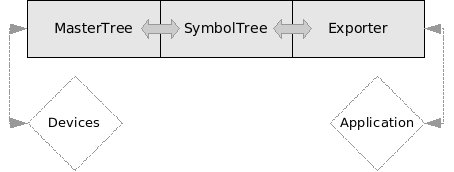
\includegraphics[scale=1]{cDCPU.png}
    \caption{Parts of the core.}
\end{figure}

The first called \textit{MasterTree}. This provide the access to the devices. The 
second part called \textit{SymbolTree} holds all values in a filesystem like 
hierachie. The last part, the \textit{Exporters}, serves the symboltree to other
applications like a visualisation. This concept is very common for this kind of 
problems. 

\subsubsection{The MasterTree}
To access the devices a master-slave based communication is often used. This are 
for example the common BUSes and also TCP/IP like networks. All these protocols
have one basic concept; they are seperable into layers. Each layer encapsulate 
an element of the communication.  For TCP/IP this is the famouse OSI reference 
model. So it is usefull to implement each layer of the communication channel
into separate modules to have the facility to reuse some of the modules. By
this you only need to implement these layers of the communication, that aren't
implemented yet to access a new device. For example if you want to access
a unsupported device that uses an allready implemented BUS you'll need only
to write a module that implements the command messages for this device.

A common way to seperate the communication is to differ between the used
interface, transport-protocol, and command-messages. The interface provides
the access to the BUS wardware, for example the serial-interface. The 
transport-protocol or BUS protocol uses the interface and generate valid 
messages that reaches the device. The module that generates the 
command-messages uses the transport-protocol to send the messages to the
device and to wait for an answer.  

\begin{figure}[ht]
    \centering
    \label{fig:cMasterTree}
    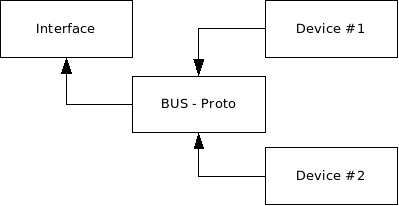
\includegraphics[scale=1]{cMasterTree.png}
    \caption{Scheme of MasterTree concept with shared interface and BUS modules.}
\end{figure}

An common cenario would be: You want to get a value from a device. So
you read from the module-object that implements the command messages.
This module will send a command-message over the BUS (protocol and interface)
to the device. Then the module will waits for an answer of the device
by reading from the BUS (over protocol and interface module). The
answer will be dispatched and you'll get the value.

If one module read from or writes to an other module the modules
will be locked and no other module can access these modules. By this way 
BUS collisions are avoided. And on the other hand if you want to access
two devices that are connected to the same BUS, you'll setup a 
MasterTree where the device-modules \#1 and \#2 share the modules for the 
interface and BUS. Now you see why the MasterTree is called a tree (forest 
would be better). The root of each tree is the interface and the leafes are 
the devices.

To get the all module work together a clear API between the modules have
to be defined, so that you don't have to adjust the modules to work together
with other/new modules. 

\subsubsection{The SymbolTree}
Once the access to the devices is seted up, you need to care about what values 
should be served. Each device will be able to provide a lot of different values
and a user or application don't know how to get a specific value. So you'll 
need a abstraction of the set of values. On the other hand, if you want to 
serve a lot of values you want to group the values by there sense and not by the
devices they are come from. So the idea of a \textit{filesystem} raises that holds 
the values in \textit{symbols} grouped in \textit{folders}, independent of the 
device the value was read from. At this point it will be usefull to control
who have access to a specific value (symbol). 

A symbol is usualy directly connected to a device-module. That means, if you 
want to get the value of the symbol, the symbol asks the device-module to read
the value from the device. But it is also possible to connect a symbol to a
module that implements a BUS protocol. By this you'll be able to tunnel the 
BUS to an other application of the internet. If you read out of such a symbol
you'll read directly from BUS and if you write into the symbol you'll write 
into the BUS. But be carefull with exporting the BUS to other networks, you
can't control what messages are sent over the BUS!

\subsubsection{Exporter}
The last part of the core exports the symboltree, or maybe a part of it, to
other applications. So the PPLT system is able to support a wide range of 
applications, independent of the protocol or interface the application
will use. Also the exporter are implemented as modules. But in this case
the comunication with the exporters are not seperated into seperate modules.
Each exporter is run into its own thread. So it is possible to handle
different applications with several instances at the same time. 


\section{Class description}
\begin{classdesc}{Core}{\optional{ModulePath, \optional{UserDBFile, \optional{LogLevel, \optional{LogFile, \optional{SysLog}}}}}}
This is the all-in-one class of the \module{pyDCPU}. All work like loding 
modules will be done by calling methods of this class. 

Creates a new core-instance. The optional argument \var{ModulePath} specifies
the basepath to the core-modules. If missed, the default path 
\texttt{sys.exec\_path+"/PPLT"} will be used. 

The argument \var{UserDBFile} specifies the filename of the used database to 
be loeded. If missed the default file 
(\texttt{sys.exec\_path+"/PPLT/UserDB.xml"}) will be used.


The argument \var{LogLevel} specifiy the loglevel and so the verbosity of the 
core. This shloud be one of (\code{'off'}, \code{'fatal'}, \code{'error'}, 
\code{'info'} or \code{'debug'}). Note that \code{'off'} switches the logging
off and \code{'debug'} will produce a lot of messages. 

In normal case all logging massages were printed on the screen (send to 
stderr) but with the arguments \var{LogFile} and \var{SysLog} you can 
manipulates this behavor. If the argument \var{LogFile} is given, this file 
will be used to log all messages to. Note, that if \var{LogFile} specified no 
messages are shown on stderr. If \var{SysLog} is \code{True} all log messages 
will be send to the local syslog-daemon. Note this argument overrides the 
setting of \var{LogFile} and also no messages were send to stderr.
\end{classdesc}

\section{Methods of \class{Core}}
\label{core-objects}
In the following section I will describe all methods of the \class{Core} 
class. 


\subsection{Mastertree methods}
\begin{methoddesc}[Core]{MasterTreeAdd}{ParentID, ModName, Address, Parameter}
This method loads an instance of a coremodule and adds it to the mastertree. 
The method returns the ID of the loaded mdoule. This ID is unique but if you 
load the same module with the same parameters, address and at the same parent, 
the ID of the allready loaded module will be returned. If an error accoures, 
the method will return \code{None}.

The argument \var{ParentID} specifies the parent-module (ID), the new loaded 
module will be attached to. If you set \var{ParentID} to \code{None} the 
module will be loaded as a root\footnote{A root-module has no parent module.}. 

The argument \var{ModName} specifies the full qualified name of the module. 
All modules are orgenized in classes and subclasses. A full qualified name 
would be a modulname with all classes and subclasses divided by single dots. 
For example: \code{Master.Interface.UniSerial} or \code{Master.Device.S7-200}.

The argument \var{Address} specifies the address used to connect the parent 
module. If there is no parent, meaning \var{ParentID} is \code{None}, or there
is no need to addressing the parentmodule, the argument \var{Address} should 
be \code{None}.

The argument \var{Parameter} specifies the parameter used to load (and setup) 
the module. This argument shlould be a dict.  The keywords are the parameters 
names (all strings) and the vlaues are the values of the singe parameter. \\ 
\note{All parameter values are strings!} If the module needs no parameters, 
please set \var{Parameter} to \code{None} or to an empty dict \code{\{\}}.
\end{methoddesc}


\begin{methoddesc}[Core]{MasterTreeDel}{ObjectID}
This method removes an (module-)object from the mastertree and destroy it. 
\note{The object mast have no chlidren, meaning no other objects  
are connected to this object.}

The argument \var{ObjectID} specifies the object you want to remove. This 
object ID is the ID you got by the \function{MasterTreeAdd()} method-call.

The method will return \code{True} if the object could be removed and destroyed 
and \code{False} otherwise.
\end{methoddesc}


\begin{methoddesc}[Core]{MasterTreeList}{ParentID}
This mehtod will list the IDs of all childen of the given moduleinstance. The argument \var{ParentID} specifies the 
ID of the moduleinstance, that children will be listed. 
\end{methoddesc}


\subsection{Symboltree methods}
\begin{methoddesc}[Core]{SymbolTreeCheckPath}{Path}
This method checks if the given \var{Path} exists. This method retuns  \code{True} if the given path is a folder or symbol
and \code{False} otherwise.
\end{methoddesc}


\begin{methoddesc}[Core]{SymbolTreeCreateFolder}{Path}
This method creates a folder. 

The argument \var{Path} specifies the full path to the folder, that will be creted. \note{The path should have the 
standrd Linux format like: \code{'/path/to/new\_folder'}.}

This method will return \code{Ture} if the folder was sucsessfully created and 
\code{False} otherwise.
\end{methoddesc}


\begin{methoddesc}[Core]{SymbolTreeCreateSymbol}{Path, ObjectID, \optional{Address}, \optional{Timeout}}
This method will creat a new symbol in the symboltree and connect it to the 
given Object.

The argument \var{Path} specifies the full path to the new symbol. This path 
should be in the standard Linux format like \code{'/path/to/new\_symbol'}.

The argument \var{ObjectID} specifies the object, the symbol will be connected
to. This is the ID you've got bach from a \function{MasterTreeAdd} call. You can 
connect a symbol to any object, but you'll not get allways usefull values back 
from this object. You can also connect the symbol to an object, that doesn't provide
any values, for example to a object of the \code{UniSerial} module to tunnel the
serial interface to an external application by the symboltree.

The optional argument \var{Address} specifies the address to be used to connect
to the object. To find out what addresses are provided by a specific module,
please look at the \textit{Core Modules Reference}. Of the address is obmitted,
no address will be used to connect to the object. In the most cases this means
to connect to the data chanel of the module. 

The optional argument \var{Timeout} specifies the cacheing time for the symbol in
seconds. The deault value is 0.5s.
For this time the last read value is returned instead of reread the value each 
time. By this it is possible to reduce the trafic on BUS if may clients access 
the symbols.
\end{methoddesc}


\begin{methoddesc}[Core]{SymbolTreeDeleteFolder}{Path}
This method will remove the given folder. This folder should be empty before removing it.

The argument \var{Path} specifies the path of the folder that will be removed. 

This method returns \code{True} on success and \code{False} on error.
\end{methoddesc}


\begin{methoddesc}[Core]{SymbolTreeDeleteSymbol}{Path}
This method will remove a symbol from the symboltree. 

The argument \var{Path} specifies the full path to the symbol, that will be removed.
This path should be in the standard Linux format like: \code{'/path/to/symbol'}.

This method will return \code{True} on success and \code{False} otherwise.
\end{methoddesc}


\begin{methoddesc}[Core]{SymbolTreeListFolder}{Path}
This method list all folders in the folder pointed by \var{Path}.

The argument \var{Path} specifies the full path to the folder, that subfolders
will be listed. 
\note{If you want to list all folders at the 
root-folder, you shloud use \code{'/'} as path.}

The method returns a list of strings or \code{None} if the path doesn't exists. The method will
return an empty list if the folder has no subfolders.
\end{methoddesc}


\begin{methoddesc}[Core]{SymbolTreeListSymbols}{Path}
This method will list all symbols in the folder pointed by \var{Path}.

The argument \var{Path} specifies the full path to the folder, that symbols
will be listed. 

\note{If you want to list all symbols at the 
root-folder, you should set \var{Path} to \code{'/'}.}

The method will return a list of strings or \code{None} if there are no 
symbols in the folder.
\end{methoddesc}


\begin{methoddesc}[Core]{SymbolTreeGetAccess}{Path}
This method will return the owner, group and accessrights of the given folder or symbol.

The argument \var{Path} specifies the path of the folder or symbol.
\end{methoddesc}


\begin{methoddesc}[Core]{SymbolTreeSetAccess}{Path, Owner, Group, Modus}
This method will set the owner, group and accessrights of the given symbol or folder.

The argument \var{Path} specifies the full path of the symbol or folder.

The argument \var{Owner} specifies the orwer of the symbol or folder, the 
argument \var{Group} specifies the group the symbol/folder will belong to.
At least the argument \var{Modus} spceifies the accessrights of the
symbol/folder.

This method will return \code{True} on success and \code{False} otherwise.
\end{methoddesc}


\begin{methoddesc}[Core]{SymbolTreeGetValue}{Path}
This method will return the value of the symbol pointed by \var{Path}.

The argument \var{Path} specifies the full path to the symbol. 

The method will return the value(s) of the symbol or \code{None} on error.
\end{methoddesc}


\begin{methoddesc}[Core]{SymbolTreeSetValue}{Path, Value}
This method will set the value of the symbol pointed by \var{Path} to \var{Value}.

The argument \var{Path} specifies the full path to the symbol, that value will be setted.

The argument \var{Value} specifies the value(s) the symbol will be setted to.

The method will return \code{True} on success or \code{False} else.
\end{methoddesc}


\subsection{Exporter methods}
\begin{methoddesc}[Core]{ExporterAdd}{ExportModule, Parameters, DefaultUser, \optional{Root='/'}}
This method will load and setup a exporter module. A exporter is something like
you may call a server.To sucessfully setup the module, some module specific 
parameters are needed. Also you can set a default user which rights will be 
used, if the exporter doesn't support any kind of authentication. Optional you can set 
a server-root. The server root should be a folder in the symbol tree. If a exporter 
is loaded with the \var{Root} option, only the symbols under the server-root 
and the subfolders of this root are exported by the server.

The argument \var{ExportModule} specifies the full qualified name of the 
exporter-module. A full qualified name kontains all classes and subclasses of 
the exporter. For example: \code{'Export.JVisu'}. 

The argument Parameters specifies the parameters, the export-module needs to be
successfully seted up. The parameters are given as a dict. The keys of the dict
are the names of the parameters and the values are the values of the 
parameters. If the export-module needs no parameters, please set 
\var{Parameters} to \code{None} or to an empty dict.

The argument \var{DefualtUser} specifies the name of the user, the server will 
get his rights from. This can be used to controll the rights of a exporter,
that doesn't know any authentication.

The optional argument \var{Root} specifies the server-root for this exporter. 
If you miss this argument or set it to \code{'/'}, the whole symboltree
will be exported by this server. Otherwise only the symbols and subfolders of
the given folder were be exported.

The method returns the ID of the exporter instance on success or \code{None}
on error.
\end{methoddesc}


\begin{methoddesc}[Core]{ExporterList}{}
This method lists the IDs of all loaded exports (servers). The method returns
a list of strings containing the IDs you got by the \function{ExporterAdd()}
methodcall. 
\end{methoddesc}


\begin{methoddesc}[Core]{ExporterDel}{ObjectID}
This method will stop and remove the exporter pointed by the given ID. 

The argument \var{ObjectID} specifies the exporter, that should be removed.
This is the ID you got by the \function{ExporterAdd} methodcall.

The method return \code{True} on success or \code{False} on error.
\end{methoddesc}

    \newcommand{\CoreModDesc}[1]{\newpage\subsection{#1}\index{Core Modules!#1}}
\newcommand{\CoreMod}[1]{\code{#1}}

\chapter{Core-modules Reference}
In this chapter I will describe all core (\module{pyDCPU}) modules.
A core module implements a new feature (protocol,device,...) to the
PPLT system. This is the atomic element of the PPLT devices and servers.

A core module is always a small python script with a specific interface 
zipped into an archive. This archive have to consists of at least two
files. One named \texttt{meta.xml} containing the meta-info of the
core-module. The second file have to be named \texttt{\_\_init\_\_.py}.
This file should include or contain the python source-code of the core
module.

In the following sections I will describe all core modules available until
now. Or all that I know of.



\section{Master modules}
Master modules are modules that are used in the PPLT devices. So this
modules implement the features to access a device, like the interface,
bus protocol, device commands, ...



%\CoreModDesc{Master.Interface.SendMail}
%This module implements the sending of e-mails via a
%specified SMTP host. \note{You have to have the permission 
%to send a e-mail of this host.} 



\CoreModDesc{Master.Interface.Socket}
This modules implements the basic TCP socket support for the PPLT system. 
With this module you can connect to other hosts over any tcp/ip based network
(Internet). This is used in the PPLT device \textit{PLC.FP-WEB} to connect to 
the tunneled ToolPort of a Panasoinc PLC. This module is able to hanle 
multible connections, so you don't need to load a 
\CoreMod{Master.Interface.Socket}-module for each connection you want.

\subsubsection{Parameters}
This module needs only one parameter:
\begin{tableiii}{l|p{10cm}|l}{textrm}{Parameter}{Description}{Default value}
\lineiii{TimeOut}
        {This parameter specifies the read-timeout for the socket 
         connection(s) in seconds. This should be a string with a floating 
         point number in it like '0.5' for a timeout of an half second.}
        {'0.0'}
\end{tableiii}

\subsubsection{Addresses}
This module need a address, thats specifies the host and port of the TCP 
connection. So if you connect to this module with an address "10.1.1.1:100"
a connection to the host "10.1.1.1" at the port 100 will be opend. See 
example for more details. \notice{If the connection to the host fails
the first time, it will be retryed each time you read/write from/to the 
module until the connection can be etablished.} 

\subsubsection{Example}
\begin{figure}[ht]
    \label{fig:coremod02}
    \centering
    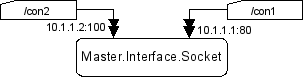
\includegraphics[scale=1]{coremod02.png}
    \caption{This figure shows the module-map of the socket-example.}
\end{figure}    
This example opens two connection to different hosts and ports:
\lstinputlisting{coremod02.py}



%
% Serial interface module:
%
\CoreModDesc{Master.Interface.UniSerial}
The \CoreMod{Master.Interface.UniSerial} core module implements the serial
interface for the PPLT system. This module needs the Python library 
\code{pySerial}. You can get this library from the URL 
\url{http://serial.sourceforge.net}. 

The settings of this module can be changed at runtime by symbols connected to
the addresses \emph{speed}, \emph{parity} \emph{timeout}.

\subsubsection{Parameters}
This module 4 parameters to setup. 
\begin{tableiii}{l|p{10cm}|l}{textrm}{Parameter}{Description}{Default value}
\lineiii{Port}
        {This is the number of the serial interface, the moudle should use. 0 
         means \code{ttyS0} or \code{COM1}, 1 means \code{ttyS1} etc. This
         parameter is not optional!}
        {---}
\lineiii{Speed}        
        {This is the speed in Baud the serial interface will be set to. This
         parameter is not optional!} 
        {---}
\lineiii{Parity}
        {This parameter specifies the parity check (settings) of the serial 
         inteface. 'Odd', 'Even', 'None' are valid values. This parameter
         is optional.}
        {'None'}
\lineiii{TimeOut}
        {This parameter sets the timeout for reading from the serial 
         interface in seconds. All floatingpoint numbers are valid an
         \code{None} means blocking-read.}
        {\code{None}}
\end{tableiii}
\notice{Some parameters can be reset at runtime by symbols connected to this 
module at special addresses. See next paragraph for details.}

\subsubsection{Addresses}
\begin{tableiii}{l|l|p{10cm}}{testrm}{Address}{Type}{Description}
\lineiii{---}
        {\code{TStream}}
        {This is the \emph{data-channel} to the serial-interface. Meaning 
         reading from this will read from the serial interface and writeing
         into a connection to this will write into the serial-interface.}
\lineiii{speed}
        {\code{TInteger}}
        {By this connector you'll be able to change the settings of the serial
         interface at runtime. Write an integer to a connection to this address
         will (try) to reset the baudrate to the value. See example for details.}
\lineiii{parity}
        {\code{TString}}
        {Writing strings like 'even', 'odd' or 'none' into this connector, will
         reset the setting of the serial interface. Reading from the connector
         will infrom you about the current setting.}
\lineiii{timeout}
        {\code{TFloat}}
        {Writing to this connector will reset the timeout for reading from 
         the serial interface.}
\end{tableiii}

\subsubsection{Example}
\begin{figure}[ht]
    \label{fig:coremod01}
    \centering
    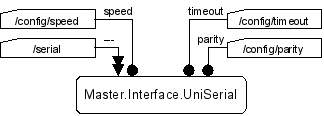
\includegraphics{coremod01.png}
    \caption{This figure shows the module-map of the UniSerial-example.}
\end{figure}    
This example shows how to setup the \CoreMod{UniSerial} and how to change the 
settings at runtime:
\lstinputlisting{coremod01.py}








%\CoreModDesc{Master.Interface.WGet}




%
% Transport layer of the Mewtocol:
%
\CoreModDesc{Master.Transport.MEWCOM-TL}
This module implements the transport-layer of the MEWTOCOL. The MEWTOCOL 
normally doesn't distinguish between the tansport and command layer. So
this module is only usfull in combination with the \CoreMod{MEWCOM-CL}
core-module that implements the command messages of the MEWTOCOL.

\subsubsection{Parameters}
This module needs only one parameter that specifies if a cecksum should
be calculated and adde to the MEWTOCOL message. By defualt this parameter
is set to \code{"True"}

\begin{tableiii}{l|p{10cm}|l}{textrm}{Parameter}{Description}{Default}
\lineiii{BCC}
        {This parameter specifies if a bcc (checksum) should be claculated
         for each packet send. This parameter doesn't contol the if the
         checksum of a recived packet will be checked. This will allways be 
         done (if the packet contains a checksum)\footnote{The MEWTOCOL 
         protocol allows that a packet doesn't contain a checksum. In this 
         case the checksum 'XX' will be set to indicate that the checksum
         should not be checked.}.  
        }{'True'}
\end{tableiii}       

\subsubsection{Addresses}
Each module or symbol have to set a address for the connection to this 
module. This address specifies the address of the destination the 
MEWTOCOL messages are send to. 
\begin{tableiii}{l|l|p{10cm}}{textrm}{Address}{Type}{Description}
\lineiii{0..255}
        {\code{TSequence}}
        {This address specifies the destination of the messages send.}
\end{tableiii}

\subsubsection{Example}
Because of this module is not usefull alone, please look at the example for 
the \CoreMod{MEWCOM-CL} core module.



%
% PPI module:
%
\CoreModDesc{Master.Transport.PPI}
This Core-Module implements the PPI protocol. It can be used to access the Siemens
SIMATIC S7 series PLCs. In this state of developing this module can't assable an
dispatch fragmentated packages. But in the most cases this is not needed. 

\subsubsection{Parameters}
This module needs only one parameter:
\begin{tableiii}{l|p{10cm}|l}{textrm}{Parameter}{Description}{Default}
\lineiii{Address}
        {This parameter specifies the PPI address of the PC. This is in the 
         most cases 0. But you have to set a value for this parameter!}
        {}
\end{tableiii}

\subsubsection{Addresses}
If you connect other modules or symbols to this module you'll need to specify
an address. This address is a number between 0 and 255. 
\begin{tableiii}{l|l|p{10cm}}{textrm}{Address}{Type}{Description}
\lineiii{0-255}{\code{Sequence}}
        {This address specifies the address of the device in the PPI BUS. 
         Writeing into the connection will cause a packet send to the device
         addressed by this address. Also reading from the connection will only
         return the content addressd to the setted Parameter \var{Address} and
         from the device addressd by this address.}
\end{tableiii}

\subsubsection{Example}
\begin{figure}[ht]
    \label{fig:coremod07}
    \centering
    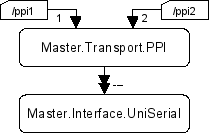
\includegraphics{coremod07.png}
    \caption{This figure shows the module-map of the PPI-example.}
\end{figure}    
This example shows how to tunnel the PPI bus by the symbol tree. For an more
usefull example please look the the Example for the \CoreMod{S7} core-module.
\lstinputlisting{coremod07.py}



%
% ReadLine module.
%
\CoreModDesc{Master.Transport.ReadLine}
This module can be used if you want to do some line-orientated communication.

This is often used for simple protocols for the serial interface. For example
the AT commands for modems but also the Mewtocol by Panasonic (FP0 and FP1) 
uses a line-orientated protocol to send or recive commands to/from the PLC.  

So this module have to be used as a child of a module that provides
\code{TStream} or \code{TSequence} connections.

\subsubsection{Parameters}
This module needs a parameter to specify the \emph{line-end} character(s).
\begin{tableiii}{l|p{10cm}|l}{textrm}{Paramter}{Description}{Default}
\lineiii{LineEnd}
        {A hex-encoded string that the module will use as a sign for the 
         line-end. And also all data send over this module will be extended
         with this string.}
        {0A0D} 
\end{tableiii}

\subsubsection{Addresses}
This module knows only one address: no address.
\begin{tableiii}{l|l|p{10cm}}{textrm}{Address}{Type}{Description}
\lineiii{---}
        {\code{TSequence}}
        {All data written into this connector will be extended by the set 
         line-end. And also if you read from this connector it will block 
         until the set line-end character(s) appear in the data-stream.
         \textbf{Note:} The whole line will be then returned!}
\end{tableiii}

\subsubsection{Example}
\begin{figure}[ht]
    \label{fig:coremod10}
    \centering
    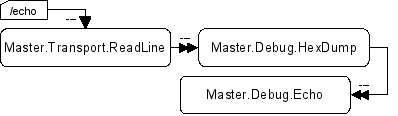
\includegraphics{coremod10.png}
    \caption{This figure shows the module-map of the ReadLine-example.}
\end{figure}    
This example shows on the one hand the usage of the \CoreMod{ReadLine} module.
On the other hand it is a quite good test for the \CoreMod{Echo} module. 
This example write a string into \CoreMod{ReadLine} that extends the string 
with the line-end. Then it will send this message to the \CoreMod{Echo} module.
Then it trys to read from \CoreMod{ReadLine} that trys to read a complete 
line from his parent (\CoreMod{Echo}) strips the line-end characters and
return the string. If all goes well the same string will be returned. To see
what's going on a \CoreMod{HexDump} module will be plugged between the 
\CoreMod{Echo} and \CoreMod{ReadLine} modules.
\lstinputlisting{coremod10.py}



%
% Agilent 5462x series oscilloscopes 
%
\CoreModDesc{Master.Device.5462X}
This module implements the command messages to access an Agilent 
oscilloscopes. This module only supports the message format used 
by the serial interface of the oscilloscope. So you need to connect
this module (indirect) to the \CoreMod{Master.Interface.UniSerial}
core-module.

\subsubsection{Parameters}
This module need two parameters to be set up. These parameters specify the
primary and secondary signal source. If you only want to use the primary
source you should set the secondary to the same source like the primary.
\begin{tableiii}{l|p{10}|l}{textrm}{Parameter}{Description}{Default}
\lineiii{PSource}
        {This specifies the primary source. This can be one of A0 (analog \#1),
         A1 (analog \#2), M (math) or F (form).}{---}
\lineiii{SSource}
        {This specifies the secondaray source. Look at \var{PSource} for more
         details}{---}
\end{tableiii}         
\bf{To be continued}\bf{To be continued}

%
% Panasonic A200 Imagechecker
%
%\CoreModDesc{Master.Device.A200}



%
% GSM compatible mobile-phone.
%
\CoreModDesc{Master.Device.GSM}



%
% Command-messages for the Panasonic FP0 and FP1
%
\CoreModDesc{Master.Device.MEWCOM-CL}
This core-module implements the command messages of the MEWTOCOL. This 
protocol is used to access the Panasonic FP0 FP2 PLCs. So you can access
the markers of these PLCs using the \CoreMod{Master.Transport.MEWCOM-TL},
\CoreMod{Master.Device.MEWCOM-CL} core-modules and a interface module like 
\CoreMod{Master.Interface.UniSerial} or \CoreMod{Master.Interface.Socket}.

\subsubsection{Parameters}
This module needs no parameters to be set up.

\subsubsection{Addresses}
You have to set a address to connect a symbol to this module! With this 
address you specify the marker you want to get/set. Additional there is a
address called \code{"STATUS"} that controls the state of the PLC 
(\emph{run}/\emph{stop}).
\begin{tableiii}{l|p{2cm}|p{10cm}}{textrm}{Address}{Type}{Description}
\lineiii{STATUS}
        {\code{TBool}}
        {By this address you can control the state of the PLC. If it is 
         \code{True} then the PLC is in the \emph{Run} mode. You can also
         get the state of the PLC by reading this value.}
\lineiii{\emph{Marker}}
        {\code{TBool} or
         \code{TInteger}}
        {By setting a marker-address as the address for the connection to this 
         module, you are able to access (read/write) this marker. So the type 
         of the connection you'll get depends on the marker-address you set.} 
\end{tableiii}

\subsubsection{Example}
\begin{figure}[ht]
    \label{fig:coremod11}
    \centering
    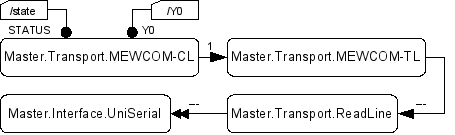
\includegraphics{coremod11.png}
    \caption{This figure shows the module-map of the MEWCOM-CL example.}
\end{figure}    
This example shows how to access a FPx using the \emph{ToolPort} (serial interface).

\lstinputlisting{coremod11.py}



%
%
%
\CoreModDesc{Master.Device.S7}
This module implements the command-messages of the Siemens SIMATIC S7(-200). 
With this module and the \CoreMod{Master.Transport.PPI} and 
\CoreMod{Master.Interface.UniSerial} it is possible to access the S7 over the 
PPI bus. To do this you must configure the serial interface in a special way. 
Look at the example to find out how. This module can generate messages that 
cause the S7 to send the value of the requested marker. To specify the marker 
you want to get you have to connect a symbol with this module with the name of
the marker as address. It could be possible that not all availabe marker can be
read. If you know some of them please let me know.

\subsubsection{Parameters}
This module needs no parameters to be set up.

\subsubsection{Addresses}
The address you have to specify to connect a symbol to this module should be 
the name of the marker you want to get/set.
\begin{tableiii}{l|p{2cm}|p{10cm}}{textrm}{Address}{Type}{Description}
\lineiii{\emph{Marker}}
        {\code{TBool}, \code{TInteger}}
        {With the address you specify the marker you'll access. So the type 
         of the values you'll get depends on the marker you'll set. So if you 
         access an boolean marker you'll get values typed \code{TBool} if you
         access byte,word and double word Markers you'll get values types
         \code{TInteger}.}
\end{tableiii}

\subsubsection{Example}
\begin{figure}[ht]
    \label{fig:coremod08}
    \centering
    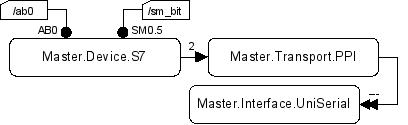
\includegraphics{coremod08.png}
    \caption{This figure shows the module-map of the S7-example.}
\end{figure}    
In this example I'll access (read/write) the markers SM0.5 (special marker 0 bit 5) and AB0
(output byte 0).

\lstinputlisting{coremod08.py}



%
% ECHO module
%
\CoreModDesc{Master.Debug.Echo}
This module echoes all data writte to it at reading from it. It can be used to
debug other modules. This is a so called \emph{root}-module. It can't be 
loaded as a child of an other module!

\subsubsection{Parameters}
This module needs no parameters!

\subsubsection{Addresses}
This module has only one addresses: no address.
\begin{tableiii}{l|l|p{10cm}}{textrm}{Address}{Type}{Description}
\lineiii{---}
        {\code{TStream}}
        {If you write into a symbol connected to this module, the data will be
         buffered and the next time you read from it the buffer (or a part of 
         it) will be returned.}
\end{tableiii}

\subsubsection{Example}
\begin{figure}[ht]
    \label{coremod06}
    \centering
    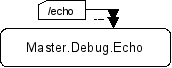
\includegraphics{coremod06.png}
    \caption{This figure shows the module-map of the Echo-example.}
\end{figure}    
This is a simple echo-example... ... the classic.

\lstinputlisting{coremod06.py}



%
% HexDump Module 
%
\CoreModDesc{Master.Debug.HexDump}
This module is a simple trafic dumper. It dumps all data going throught it
into the logging-system with loglevel \emph{debug}. So you can read it from
your logfile or \code{stderr}. Simply plug this module between two modules
to record all trafic.

\subsubsection{Parameters}
This module needs no parameters!

\subsubsection{Addresses}
This module has only one address: no address! 
\begin{tableiii}{l|p{2cm}|p{10cm}}{textrm}{Address}{Type}{Description}
\lineiii{---}
        {\code{TStream} or \code{TSequence}}
        {All data written to this module will be written to the parent and 
         read vica versa. So the type of the connection will depend on the
         type of the parent-connection.}
\end{tableiii}

\subsubsection{Example}
\begin{figure}[ht]
    \label{fig:coremod05.py}
    \centering
    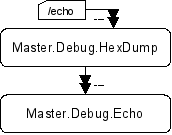
\includegraphics{coremod05.png}
    \caption{This figure shows the module-map of the HexDump-example.}
\end{figure}    
This module uses the echo module to show how the trafic in read and write 
direction will be dumped:
\lstinputlisting{coremod05.py}



%
% Null module (the black hole)
%
\CoreModDesc{Master.Debug.Null}
This is a very simple module, that works like the /dev/null device file on 
Linux. If you read from this module, you'll get a string with zero-bits and
if you write into this module nothing will happens. This module swallow all
you write into it.

\subsubsection{Parameters}
This module needs no parameters to be set up.

\subsubsection{Addresses}
This module has only one valid address: no address.
\begin{tableiii}{l|l|p{10cm}}{textrm}{Address}{Type}{Description}
\lineiii{---}
        {\code{TStream}}
        {This will be the connection to the \CoreMod{Null} module. Id you
         write into this connection the module will swallow all data and
         nothing will happen. If you read from this module you'll get a 
         stream of zero-bits.}
\end{tableiii}

\subsubsection{Example}
\begin{figure}[ht]
    \label{fig:coremod09}
    \centering
    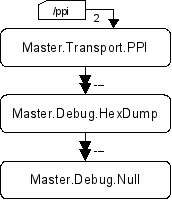
\includegraphics{coremod09.png}
    \caption{This figure shows the module-map of the Null-Example.}
\end{figure}    
This example shows a configuration to debug a non \emph{root} module. In this 
case it is the \CoreMod{Master.Transport.PPI} core-module. To get some 
information about the packages the PPI module sends the core-module 
\CoreMod{Master.Debug.HexDump} is used.  \notice{This example raises an 
exception, because the PPI module expect a correct answer from the 
\emph{virtual} device (in this case the core-module 
\CoreMod{Master.Debug.Null}).
\lstinputlisting{coremod09.py}



%
% Random-generator module
%
\CoreModDesc{Master.Debug.Random}
This module implements a random-generator, that can generate data for every 
symbol-type supported by the \module{pyDCPU}. So this module can be used to 
test almost all facilities of the system. 

\subsubsection{Parameters}
This module needs no parameters. 

\subsubsection{Addresses}
\begin{tableiii}{l|l|p{10cm}}{testrm}{Address}{Type}{Description}
\lineiii{Bool}
        {\code{TBool}}
        {Provide a random boolean value.}
\lineiii{Integer}
        {\code{TInteger}}
        {Provide a random integer value between 0 and 100.}
\lineiii{Float}
        {\code{TFloat}}
        {Provide a random floating point number between 0 and 1.}
\lineiii{String}
        {\code{TString}}
        {Provide a random string of a random length between 1 and 79 containg 
         printable characters.}
\lineiii{ArrayBool}
        {\code{TArrayOfBool}}
        {The name tells everything. The length of the array is randomly 
         between 1 and 3.}
\lineiii{ArrayInteger}
        {\code{TArrayOfInteger}}
        {Array of integer of random length between 1 and 3.}
\lineiii{ArrayFloat}
        {\code{TArrayOfFloat}}
        {Array of floating point numbers with variable length between 1 and 
         3.}
\lineiii{ArrayString}
        {\code{TArrayOfString}}
        {Array of string with variable length (of array) between 1 and 3.}
\lineiii{Stream}
        {\code{TStream}}
        {Provides an random data string. The data are printable character.
         The number of bytes returned is less than equeal the number you 
         wanted to read. To read from a symbol connected to this address,
         please use the method \method{SymbolTreeRead().}}
\lineiii{Sequence}
        {\code{TSequence}}
        {A sequence of random data. The data contains only printable 
         characters and the length varies between 1 and 79.}
\end{tableiii}

\subsubsection{Example}
This is a simple example that uses all types:
\lstinputlisting{coremod03.py}



%
% Statistic module
%
\CoreModDesc{Master.Debug.Statistic}
This module collects statistical values of the data flowing through it. You 
can use this module to improve or debug your own modules or even to observe
the PPLT system. This module is quite easy to use: simply plug this between 
two other modules and you are able to observe the trafic between them.
\notice{You can only observe modules that provides a \code{TStream} or 
\code {TSequence} connection.}

\subsubsection{Parameters}
This module needs no parameters!

\subsubsection{Addresses}
There are several addresses provideing the statistical data. If you use no 
address to connect to this module a \code{TStream} or \code{TSequence} 
connection to the parent will be returned. This connection to the parent will
be used to collect the statistical data. 

\begin{tableiii}{l|p{2cm}|p{10cm}}{textrm}{Address}{Type}{Description}
\lineiii{---}
        {\code{TStream} or \code{TSequence}}
        {This is the data-tunnel to the parent of the 
         \CoreMod{Statistic}-module. The type of the connection depends on
         the type of the connection to the parent module. You see, it is only
         possible to connect the \CoreMod{Statistic}-module to a parent that
         provides a \code{TStream} or \code{TSequence} connection.}
\lineiii{read\_data}
        {\code{TInteger}}
        {Returns the number of bytes read from the parent.}
\lineiii{write\_data}
        {\code{TInteger}}
        {Returns the number of bytes written to the parent.}
\lineiii{read\_speed}
        {\code{TFloat}}
        {Returns the number of bytes per second read from parent since 
         module-loading. This value is the average of the whole time since
         module-loading.}
\lineiii{write\_speed}
        {\code{TFloat}}
        {Returns the number of bytes written to the parent since the module 
        was loaded. This value is the average of the whole time.}
\lineiii{error}
        {\code{TInteger}}
        {Returns the number of read/write-errors since the module was loaded.
         This must not be an indicatior for bugs in the parent modules because
         also timeouts will be recorded.}
\end{tableiii}

\subsubsection{Example}
In this example the serial interface will be exported by the symbol tree.
The \CoreMod{Statistic}-module records the trafic throught the serial 
interface.
\lstinputlisting{coremod04.py}



\newpage
\section{Export modules}
\CoreModDesc{Export.JVisu}
\CoreModDesc{Export.SimpleExport}
\CoreModDesc{Export.PPLTWeb}


    
    
    \newcommand{\PSFTag}[1]{\index{PSF Elements!#1}}



\chapter{PSF Reference --- \textbf{P}PLT \textbf{S}ession \textbf{F}ile}

This section describes the file-format of the PPLT session files. Such 
files contain the information about the state of the system. 
So the file contains information about the loaded devices and servers and
also the layout of the symbol-tree.

Files formatted in the PSF format can be created from a running PPLT system by 
a call of the method \method{SaveSession()} and can then be loaded by a 
\method{LoadSession()} method-call.

By this way you can easily implement a simple daemon or service, that reads 
such a PSF file and setup a whole PPLT system. Meaning loading all devices, 
creating all symbols and folders and at the end loading all servers.

All you need to know is a basic knowledge of XML formats, and a little idea of 
what PPLT is and what the system needs to save (or even needs to know to setup
the PPLT system). 

\section{Reference}
In the following section I'll list all keyword of the PSF format. These are only few
because the format stills easy. 

At first: The PSF format is an XML format!

\subsection{\keyword{PPLTSession}}
\PSFTag{PPLTSession}
The PPLTSession tags surround the PPLT session document. Containing all 
information about the devices, servers and symbol-tree. This tag must
(directly) contain the elements (tags) \keyword{Servers}, \keyword{Devices}
and \keyword{SymbolTree}. But each elements can only occur once.
This also defines the basic layout of the PPLT session document. Each document
should look like:
\begin{verbatim}
<?xml version="1.0"?>
<PPLTSession>
    <Servers>
        [...]
    </Servers>
    <Devices>
        [...]
    </Devices>
    <SymbolTree>
        [...]
    </SymbolTree>
</PPLTSession>
\end{verbatim}


\subsection{\keyword{Servers}}
\PSFTag{Servers}
The tag \keyword{Servers} contains the description of all loaded servers. This tag can only 
contain any occurrence of the tag \keyword{Server}. Each \keyword{Server}-tag describe a 
singe server to load. For more details see at the description of the \keyword{Server}-tag.

\begin{verbatim}
[...]
    <Servers>
        <Server [...]>
            [...]
        </Server>
        [...]
    </Servers>
[...]
\end{verbatim}


\subsection{\keyword{Server}}
\PSFTag{Server}
The tag \keyword{Server} describes a server to load. The tag can only contain any occurrence of the tag
\keyword{Parameter}. Each \keyword{Parameter} tag specifies a parameter needed to load the server.
Also the \keyword{Server} needs some attributes. The attribute \var{alias} specifies the alias the
server will get after it was loaded. The attribute \var{fqsn} specifies the full-qualified-server-name. 
This unique name specifies the server to be loaded. The Attribute \var{root} specifies the server root.
\note{The given server-root but exist else the loading of the server will fail.} The attribute 
\var{user} specifies the default user. The server will run with the rights of this user, if the 
server doesn't know any authentication. 

A simple example will can be:
\begin{verbatim}
[...]
    <Server alias="JVisu" fqsn="Visu.JVisuServer" root="/" user="admin">
        <Parameter name="Port">2200</Parameter>
        <Parameter name="Address">127.0.0.1</Parameter>
    </Server>
[...]
\end{verbatim}
This example will start a JVisu server with the rights of the user \code{admin} and
with the server root \code{'/'}. JVisu is a open source visualization written in Java.
You can get it from \url{http://jvisu.sourceforge.net}.

\subsection{\keyword{Parameter}}
\PSFTag{Parameter}
The \keyword{Parameter}-tag specifies a parameter, the system will use to setup
a \keyword{Server} or \keyword{Device}. The \keyword{Parameter}-tag can only 
contain CDATA, meaning it can only contain a string. The content will be 
interpreted as the value of the parameter. The \keyword{Parameter}-tag
knows also a attribute. The attribute \var{name} specifies the name
of the parameter. To find out what parameters are needed to setup
a specific server, please consult the Device and Server reference.


\subsection{\keyword{Devices}}
\PSFTag{Devices}
Like the \keyword{Servers}-tag this tag contains the description of
all devices needed to be loaded. So this tag can only contain any
occurrence of the tag \keyword{Device}. For example:
\begin{verbatim}
[...]
    <Devices>
        <Device [...]>
            [...]
        </Device>
        [...]
    </Devices>
[...]
\end{verbatim}


\subsection{\keyword{Device}}
\PSFTag{Device}
Like the \keyword{Server}-tag this tag describes one device to load. Also it can only contain 
any number of \keyword{Parameter} tags to specify the the parameters the device may need to be
loaded. It also has some attributes. The attribute \var{alias} specifies the alias the device 
gets when it's was successfully loaded. The attribute \var{fqdn} specifies the full qualified 
device name. This is the name of the device you want to load.

For example, a \keyword{Devices}-section can be:
\begin{verbatim}
[...]
    <Devices>
        <Device alias="rand" fqdn="Debug.RandomGenerator"/>
        <Device alias="S7" fqdn="PLC.S7-200">
            <Parameter name="PCAddr">0</Parameter>
            <Parameter name="Port">1</Parameter>
            <Parameter name="S7Addr">2</Parameter>
        </Device>
    </Devices>
[...]
\end{verbatim}
This example will load a random-generator as \code{'rand'}  and the support for the Siemens SIMATIC S7-200 
as \code{'S7'}.


\subsection{\keyword{SymbolTree}}
\PSFTag{SymbolTree}
The \keyword{SymbolTree}-section describes the content of the symbol-tree. So this tag can only contain
any occurrence of \keyword{Symbol} and \keyword{Folder} tags. This tag don't take any attributes.

\subsubsection{How the symbol-tree is depicted}
The symbol-tree works like a small filesystem, with folders, sub-folder and symbols. The root of this filesystem is the
symbol-tree itself. Now you need to know how to depict the hierarchy of the symbol-tree to an XML file.

I think the best way to describe is to give an example. The following symbol-tree hierarchy
\begin{verbatim}
/
/FOLDER1/
/FOLDER1/FOLDER2/
/FOLDER1/FOLDER2/Symbol1
/FOLDER1/FOLDER2/Symbol2
/FOLDER1/Symbol3
/FOLDER3/
/FOLDER3/Symbol4
/Symbol5
\end{verbatim}
will be depicted as something like:
\begin{verbatim}
<SymbolTree>
    <Folder name="FOLDER1">
        <Folder name="FOLDER2">
            <Symbol name="Symbol1"/>
            <Symbol name="Symbol2"/>
        </Folder>
        <Symbol name="Symbol3"/>
    </Folder>    
    <Folder name="FOLDER3">
        <Symbol name="Symbol4"/>
    </Folder>
    <Symbol name="Symbol5"/>
</SymbolTree>
\end{verbatim}
As you see; the \keyword{SymbolTree} can contain \keyword{Symbol}s and \keyword{Folder}s. And each \keyword{Folder} can
also contain \keyword{Symbol}s and \keyword{Folder}s. But only the \keyword{Symbol}s are empty, because they can't contain
anything. In this example I missed some additional attributes to avoid you to be confused. This attributes are described 
in detail in the following sections.

\subsection{\keyword{Symbol}}
\PSFTag{Symbol}
The \keyword{Symbol}-tag describes a symbol of the symbol-tree. Such a symbol is a kind of a variable that can hold values.
Each symbol is connected to a so called "symbol-slot"\footnote{A symbol-slot always belongs to a device, so if you want to know 
what slots are provided by a specific device, pleas look at the documentation of the device.}. So you need to specify the 
symbol-slot the symbol will be connected to by the attribute \var{slot}. The slot-name must be provided in the format 
\code{'DEVICE\_ALIAS::NAMESPACE::SLOT\_NAME'}. The \code{DEVICE\_ALIAS} specifies the device you want the symbol to be
connected to. It should be the string you give to the \keyword{Device}-attribute \var{alias}. The \code{NAMESPACE}s and
\code{SLOT\_NAME}s are provided by the devices. To find out what namespaces are available, look at the documentation of 
each device.

In this context you also need to define the type of the symbol by the attribute \var{type}. The type is defined by the
slot you use. So please take a look at the documentation of the specific device.

Now your symbol can get and (maybe) set values. But a major feature of the PPLT is, that you can control the
access to the symbol by setting rights to it. To do so, you need to set a \var{owner}, \var{group} and
\var{modus} to the symbol (and also to the folder). So a complete example for a symbol that is connected to
a random-generator loaded as \code{'rand'} could be:
\begin{verbatim}
[...]
    <SymbolTree>
        <Symbol name="r_bool" slot="rand::Generator::Bool" type="Bool" 
                owner="admin" group="Admin" modus="600"/>
        [...]
    </SymbolTree>
[...]
\end{verbatim}
You see the attribute \var{modus} contains a 3-digit integer. This integer is calculated like the Linux modus integer. Pleas look
at the \manpage{chmod}{} man-page to get more information. But sofar the number \code{600} says that only the owner has the right to 
read/write to the symbol and the group and any other has no rights.


\subsection{\keyword{Folder}}
\PSFTag{Folder}
The \keyword{Folder}-tag describes a folder in the symbol-tree. The name of the folder will be specified by the
attribute \var{name}. Like the symbols a folder also owned by a user and attached to a group. So you also need 
to set the \var{owner}, \var{group} and \var{modus} attributes. 

\newpage
\section{A complete Example}
In the following section I'll show you a complete example of a PSF. The file describes two devices, a random generator and
a Siemens SIMATIC S7-200. The symbol-tree contains two folders one, named 'Rand', will contain some symbols connected
to the random-generator and the other, named 'S7' will contains the symbols connected to the S7. And a web-server will be loaded, 
that exports the whole symbol-tree. 

\verbatiminput{PSF.xml}



    
    \documentclass{manual}

\title{PPLT References}
\author{Hannes Matuschek\\\texttt{<hmatuschek@gmx.net>}}
%\date{2005-10-12}
\release{0.9.0}
\setshortversion{0.9.0(beta)}
\makeindex


 \begin{document}
   
    \maketitle
    \begin{abstract}
    This document summarize the references of the PPLT system. Including Core-Library reference, reference
    of the PPLT abstraction layer, documenttypes and some other stuff.
    \end{abstract}

    \tableofcontents


    \input{PPLTReference}
    \input{PPLTModRef}
    
    \input{CoreReference}
    \input{CoreModRef}
    
    
    \input{PSFReference}
    
    \input{Reference.ind}
 \end{document}

 \end{document}

 \end{document}

 \end{document}
